\documentclass{article}
%DIF LATEXDIFF DIFFERENCE FILE
%DIF DEL original.tex    Mon Nov  9 15:27:43 2026
%DIF ADD revisions.tex   Mon Nov  9 16:06:11 2026

\usepackage{arxiv}

\usepackage[utf8]{inputenc} % allow utf-8 input
\usepackage[T1]{fontenc}    % use 8-bit T1 fonts
\usepackage{hyperref}       % hyperlinks
\usepackage{url}            % simple URL typesetting
%DIF 9a9
\usepackage{xurl}           % allow line breaks anywhere in long URLs %DIF > 
%DIF -------
\usepackage{booktabs}       % professional-quality tables
\usepackage{amsfonts}       % blackboard math symbols
\usepackage{amsmath}        % equations
\usepackage{nicefrac}       % compact symbols for 1/2, etc.
\usepackage{microtype}      % microtypography
\usepackage{graphicx}
%DIF 15c16-17
%DIF < \usepackage[numbers]{natbib}
%DIF -------
\usepackage[numbers,sort&compress]{natbib} %DIF > 
\usepackage{longtable} %DIF > 
%DIF -------
\usepackage{doi}
%DIF 17a19-20
\usepackage[mathlines]{lineno} %DIF > 
\linenumbers %DIF > 
%DIF -------

\title{\DIFdelbegin \DIFdel{Evidence of fault zone transport of road-salt contaminated groundwater from highways to streams}\DIFdelend \DIFaddbegin \DIFadd{Do fault zones route road-salt-contaminated groundwater to streams? A Hudson Valley, NY Case Study}\DIFaddend }

%DIF 20-22d24
%DIF < % TODO: The source docx contains no author block. Names below are from the
%DIF < % project record (senior honors thesis at Marist); fill in departments,
%DIF < % emails, and ORCIDs before submission.
%DIF -------
\author{
	\DIFdelbegin \DIFdel{Tadd Bindas }\DIFdelend \DIFaddbegin \href{https://orcid.org/0000-0003-3159-6276}{
\includegraphics[scale=0.06]{orcid.pdf}\DIFadd{\hspace{1mm}Tadd Bindas}} \DIFaddend \\
	\DIFaddbegin \DIFadd{Marist University}\\
	\DIFadd{Poughkeepsie, NY }\\
	\DIFaddend \texttt{taddbindas@gmail.com} \\
	\And
	\DIFdelbegin \DIFdel{Zion Klos }\DIFdelend \DIFaddbegin \href{https://orcid.org/0000-0002-9563-6065}{
\includegraphics[scale=0.06]{orcid.pdf}\DIFadd{\hspace{1mm}Zion Klos}} \DIFaddend \\
	Marist University\\
	Poughkeepsie, NY \\
	\texttt{zion.klos@marist.edu} \\
}

\date{}

%DIF 37c38-40
%DIF < \renewcommand{\shorttitle}{Fault zone transport of road-salt contaminated groundwater}
%DIF -------
\renewcommand{\shorttitle}{Do fault zones route road-salt-contaminated groundwater to streams?} %DIF > 
\renewcommand{\headeright}{} %DIF > 
\renewcommand{\undertitle}{} %DIF > 
%DIF -------

\hypersetup{
%DIF 40c43
%DIF < pdftitle={Evidence of fault zone transport of road-salt contaminated groundwater from highways to streams},
%DIF -------
pdftitle={Do fault zones route road-salt-contaminated groundwater to streams? A Hudson Valley, NY Case Study}, %DIF > 
%DIF -------
pdfauthor={Tadd Bindas, Zion Klos},
pdfkeywords={water quality, fault lines, salinity, de-icing, roadway management},
}
%DIF PREAMBLE EXTENSION ADDED BY LATEXDIFF
%DIF UNDERLINE PREAMBLE %DIF PREAMBLE
\RequirePackage[normalem]{ulem} %DIF PREAMBLE
\RequirePackage{color}\definecolor{RED}{rgb}{1,0,0}\definecolor{BLUE}{rgb}{0,0,1} %DIF PREAMBLE
\providecommand{\DIFaddtex}[1]{{\protect\color{blue}\uwave{#1}}} %DIF PREAMBLE
\providecommand{\DIFdeltex}[1]{{\protect\color{red}\sout{#1}}} %DIF PREAMBLE
%DIF SAFE PREAMBLE %DIF PREAMBLE
\providecommand{\DIFaddbegin}{} %DIF PREAMBLE
\providecommand{\DIFaddend}{} %DIF PREAMBLE
\providecommand{\DIFdelbegin}{} %DIF PREAMBLE
\providecommand{\DIFdelend}{} %DIF PREAMBLE
\providecommand{\DIFmodbegin}{} %DIF PREAMBLE
\providecommand{\DIFmodend}{} %DIF PREAMBLE
%DIF FLOATSAFE PREAMBLE %DIF PREAMBLE
\providecommand{\DIFaddFL}[1]{\DIFadd{#1}} %DIF PREAMBLE
\providecommand{\DIFdelFL}[1]{\DIFdel{#1}} %DIF PREAMBLE
\providecommand{\DIFaddbeginFL}{} %DIF PREAMBLE
\providecommand{\DIFaddendFL}{} %DIF PREAMBLE
\providecommand{\DIFdelbeginFL}{} %DIF PREAMBLE
\providecommand{\DIFdelendFL}{} %DIF PREAMBLE
%DIF HYPERREF PREAMBLE %DIF PREAMBLE
\providecommand{\DIFadd}[1]{\texorpdfstring{\DIFaddtex{#1}}{#1}} %DIF PREAMBLE
\providecommand{\DIFdel}[1]{\texorpdfstring{\DIFdeltex{#1}}{}} %DIF PREAMBLE
\providecommand{\DIFscaledelfig}{0.5}
%DIF HIGHLIGHTGRAPHICS PREAMBLE %DIF PREAMBLE
\RequirePackage{settobox} %DIF PREAMBLE
\RequirePackage{letltxmacro} %DIF PREAMBLE
\newsavebox{\DIFdelgraphicsbox} %DIF PREAMBLE
\newlength{\DIFdelgraphicswidth} %DIF PREAMBLE
\newlength{\DIFdelgraphicsheight} %DIF PREAMBLE
% store original definition of \includegraphics %DIF PREAMBLE
\LetLtxMacro{\DIFOincludegraphics}{\includegraphics} %DIF PREAMBLE
\providecommand{\DIFaddincludegraphics}[2][]{{\color{blue}\fbox{\DIFOincludegraphics[#1]{#2}}}} %DIF PREAMBLE
\providecommand{\DIFdelincludegraphics}[2][]{% %DIF PREAMBLE
\sbox{\DIFdelgraphicsbox}{\DIFOincludegraphics[#1]{#2}}% %DIF PREAMBLE
\settoboxwidth{\DIFdelgraphicswidth}{\DIFdelgraphicsbox} %DIF PREAMBLE
\settoboxtotalheight{\DIFdelgraphicsheight}{\DIFdelgraphicsbox} %DIF PREAMBLE
\scalebox{\DIFscaledelfig}{% %DIF PREAMBLE
\parbox[b]{\DIFdelgraphicswidth}{\usebox{\DIFdelgraphicsbox}\\[-\baselineskip] \rule{\DIFdelgraphicswidth}{0em}}\llap{\resizebox{\DIFdelgraphicswidth}{\DIFdelgraphicsheight}{% %DIF PREAMBLE
\setlength{\unitlength}{\DIFdelgraphicswidth}% %DIF PREAMBLE
\begin{picture}(1,1)% %DIF PREAMBLE
\thicklines\linethickness{2pt} %DIF PREAMBLE
{\color[rgb]{1,0,0}\put(0,0){\framebox(1,1){}}}% %DIF PREAMBLE
{\color[rgb]{1,0,0}\put(0,0){\line( 1,1){1}}}% %DIF PREAMBLE
{\color[rgb]{1,0,0}\put(0,1){\line(1,-1){1}}}% %DIF PREAMBLE
\end{picture}% %DIF PREAMBLE
}\hspace*{3pt}}} %DIF PREAMBLE
} %DIF PREAMBLE
\LetLtxMacro{\DIFOaddbegin}{\DIFaddbegin} %DIF PREAMBLE
\LetLtxMacro{\DIFOaddend}{\DIFaddend} %DIF PREAMBLE
\LetLtxMacro{\DIFOdelbegin}{\DIFdelbegin} %DIF PREAMBLE
\LetLtxMacro{\DIFOdelend}{\DIFdelend} %DIF PREAMBLE
\DeclareRobustCommand{\DIFaddbegin}{\DIFOaddbegin \let\includegraphics\DIFaddincludegraphics} %DIF PREAMBLE
\DeclareRobustCommand{\DIFaddend}{\DIFOaddend \let\includegraphics\DIFOincludegraphics} %DIF PREAMBLE
\DeclareRobustCommand{\DIFdelbegin}{\DIFOdelbegin \let\includegraphics\DIFdelincludegraphics} %DIF PREAMBLE
\DeclareRobustCommand{\DIFdelend}{\DIFOaddend \let\includegraphics\DIFOincludegraphics} %DIF PREAMBLE
\LetLtxMacro{\DIFOaddbeginFL}{\DIFaddbeginFL} %DIF PREAMBLE
\LetLtxMacro{\DIFOaddendFL}{\DIFaddendFL} %DIF PREAMBLE
\LetLtxMacro{\DIFOdelbeginFL}{\DIFdelbeginFL} %DIF PREAMBLE
\LetLtxMacro{\DIFOdelendFL}{\DIFdelendFL} %DIF PREAMBLE
\DeclareRobustCommand{\DIFaddbeginFL}{\DIFOaddbeginFL \let\includegraphics\DIFaddincludegraphics} %DIF PREAMBLE
\DeclareRobustCommand{\DIFaddendFL}{\DIFOaddendFL \let\includegraphics\DIFOincludegraphics} %DIF PREAMBLE
\DeclareRobustCommand{\DIFdelbeginFL}{\DIFOdelbeginFL \let\includegraphics\DIFdelincludegraphics} %DIF PREAMBLE
\DeclareRobustCommand{\DIFdelendFL}{\DIFOaddendFL \let\includegraphics\DIFOincludegraphics} %DIF PREAMBLE
%DIF AMSMATHULEM PREAMBLE %DIF PREAMBLE
\makeatletter %DIF PREAMBLE
\let\sout@orig\sout %DIF PREAMBLE
\renewcommand{\sout}[1]{\ifmmode\text{\sout@orig{\ensuremath{#1}}}\else\sout@orig{#1}\fi} %DIF PREAMBLE
\makeatother %DIF PREAMBLE
%DIF END PREAMBLE EXTENSION ADDED BY LATEXDIFF

\begin{document}
\maketitle

\begin{abstract}
\DIFdelbegin \DIFdel{Many streams in }\DIFdelend \DIFaddbegin \DIFadd{Road salt applied to highways has salinized streams across }\DIFaddend the northeastern United States\DIFdelbegin \DIFdel{have grown saltier over recent decades, a trend tied to the widespread use of salt as a road deicer and now recognized as one facet of a broader freshwater salinization syndrome. These rising salt concentrations degrade water quality and stress freshwater ecosystems. Rather than declining in summer, when little salt is applied, stream salinity often rises during these low-flow periods, when groundwater supplies most of the streamflow. This pattern reflects a legacy of road salt stored in and slowly released from groundwater, and it raises the question of what controls where that stored salt re-emerges. We hypothesized that high-angle geologic fault zones act as preferential conduits that rapidly route road-salt-contaminated groundwaterfrom highways to streams, potentially over kilometers and beneath topographic divides, a linkage previously inferred only from groundwater wells. We tested this with dense longitudinal surveys of }\DIFdelend \DIFaddbegin \DIFadd{, and much of that salt is stored in groundwater and released to streams for years to decades, keeping stream salinity high even during summer baseflow. Where this stored salt re-enters streams is poorly understood. High-angle geologic faults are one candidate pathway: their fractured damage zones can channel groundwater, and road salt has been traced into fractured-bedrock wells, where it persists year-round. However, it has not been tested whether faults deliver this water to streams at locations a stream survey can detect. We asked whether mapped faults in the Hudson Valley, New York, coincide with abrupt increases in stream }\DIFaddend specific conductance, \DIFdelbegin \DIFdel{together with a targeted chloride transect, }\DIFdelend \DIFaddbegin \DIFadd{a proxy for salinity. We surveyed specific conductance }\DIFaddend along three reaches of Wappinger Creek \DIFdelbegin \DIFdel{in Dutchess County, New York, where mapped faults cross the channel. Of the }\DIFdelend \DIFaddbegin \DIFadd{crossed by mapped faults, compared reaches upstream and downstream of fault crossings and tributary junctions, applied change-point analysis to locate where conductance changed, and measured one chloride transect. Comparisons were valid only within a single survey day: pooling two survey days created an apparent 18~$\mu$S/cm step at one fault that fell to a non-significant 1.6~$\mu$S/cm within a day. Of }\DIFaddend three fault crossings\DIFdelbegin \DIFdel{not confounded by a coincident tributary, two showed statistically significant increases in specific conductance across the fault ($\alpha$ = 0.05}\DIFdelend \DIFaddbegin \DIFadd{, only one showed a small significant increase (4.3~$\mu$S/cm}\DIFaddend ), and \DIFdelbegin \DIFdel{an independent chloride transect reproduced the strongest of these steps at the same mapped fault. From this case study we find spatially explicit evidence that faultzones can concentrate the delivery of road-salt-contaminated groundwater to streams. Because comparable faults are already mapped throughout the region, we argue that known fault locations should be incorporated into both roadway and water-quality management planning. }\DIFdelend \DIFaddbegin \DIFadd{it was a gradual rise beginning about 1.6~km upstream rather than a step at the fault. No conductance breakpoint coincided with a fault, while tributary junctions lowered conductance as mixing predicts. Road proximity, wastewater discharges and salt stored in soils remain plausible alternative sources. This low-cost survey therefore does not clearly show fault-routed transport. We outline a falsifiable test combining single-day surveys, discharge measurements, chloride-to-bromide ratios, age tracers and field-located faults.
}\DIFaddend \end{abstract}

\keywords{water quality \and fault lines \and salinity \and de-icing \and roadway management}

\section{Introduction}

\DIFdelbegin \DIFdel{Introduced in the early 1940s as a road }\DIFdelend \DIFaddbegin \DIFadd{Road salt has been used as a }\DIFaddend de-icing agent in \DIFdelbegin \DIFdel{North America and Europe, road salt's usage }\DIFdelend \DIFaddbegin \DIFadd{the United States since the 1940s, and its use }\DIFaddend has climbed steadily decade over decade \DIFdelbegin \DIFdel{\mbox{%DIFAUXCMD
\citep{tiwari2018,bubeck1971,jackson2005}}\hskip0pt%DIFAUXCMD
, becoming }\DIFdelend \DIFaddbegin \DIFadd{\mbox{%DIFAUXCMD
\citep{tiwari2018,jackson2005}}\hskip0pt%DIFAUXCMD
. It is }\DIFaddend indispensable for winter road safety\DIFdelbegin \DIFdel{. However, it introduces }\DIFdelend \DIFaddbegin \DIFadd{, but it also poses }\DIFaddend a widespread salinization threat to fresh waters across cold-climate regions \citep{kaushal2005,dugan2023}. \DIFdelbegin \DIFdel{Road salts are effective only within a temperature window; below roughly $-9.5$~$^{\circ}$C (15~$^{\circ}$F) it becomes marginally effective, melting demands very high application rates , and most transportation agencies advise against its use \mbox{%DIFAUXCMD
\citep{kelting2010}}\hskip0pt%DIFAUXCMD
. In practice, it is nonetheless applied under these conditions and in amounts beyond what de-icing requires, with consequences that reach well beyond the roadway \mbox{%DIFAUXCMD
\citep{jamshidi2020}}\hskip0pt%DIFAUXCMD
. }%DIFDELCMD < 

%DIFDELCMD < %%%
\DIFdel{Structurally, road salts have corrosive effects that accelerate damage to automobiles, bridges, and other infrastructure \mbox{%DIFAUXCMD
\citep{kelting2010}}\hskip0pt%DIFAUXCMD
. Environmentally, they contaminate groundwater and degrade }\DIFdelend \DIFaddbegin \DIFadd{Application rates vary widely between jurisdictions \mbox{%DIFAUXCMD
\citep{jamshidi2020}}\hskip0pt%DIFAUXCMD
. Beyond corroding vehicles and infrastructure \mbox{%DIFAUXCMD
\citep{kelting2010}}\hskip0pt%DIFAUXCMD
, road salt contaminates groundwater and degrades }\DIFaddend stream water quality \citep{jackson2005,williams1999}\DIFdelbegin \DIFdel{. Their documented ecological effects range from salt-tolerant invasive species outbreaks \mbox{%DIFAUXCMD
\citep{richburg2001} }\hskip0pt%DIFAUXCMD
and disruption of roadside and aquatic habitat \mbox{%DIFAUXCMD
\citep{forman1998} }\hskip0pt%DIFAUXCMD
to }\DIFdelend \DIFaddbegin \DIFadd{, with ecological effects that include }\DIFaddend longer-term \DIFdelbegin \DIFdel{, indirect }\DIFdelend shifts in ecosystem function \citep{findlay2011}. \DIFdelbegin \DIFdel{Many of these effects propagate through aquatic food webs via osmoregulatory stress and community-level feedbacks, and they }\DIFdelend \DIFaddbegin \DIFadd{These effects }\DIFaddend occur at chloride concentrations at or below existing regulatory guidelines: \DIFdelbegin \DIFdel{in a coordinated experiment spanning lakes in North America and Europe, }\DIFdelend \citet{hintz2022} found that chloride \DIFdelbegin \DIFdel{levels }\DIFdelend at or beneath current water-quality thresholds caused substantial losses of zooplankton \DIFdelbegin \DIFdel{and, at nearly half of the study sites, cascading increases in phytoplankton. Because present guidelines do not reliably protect freshwater ecosystems, identifying }\DIFdelend \DIFaddbegin \DIFadd{in lakes across North America and Europe. Identifying }\DIFaddend \emph{where} salt enters streams, and therefore where mitigation would be most effective, \DIFaddbegin \DIFadd{thus }\DIFaddend carries direct management value.

Although road salt is applied only in the cold months, its effects on freshwater salinity extend across the entire year \citep{shattuck2023}. \DIFdelbegin \DIFdel{While chloride }\DIFdelend \DIFaddbegin \DIFadd{Chloride }\DIFaddend concentrations are highest in \DIFdelbegin \DIFdel{the }\DIFdelend winter \citep{corsi2015}, \DIFdelbegin \DIFdel{road salts persist in soil for a minimum of 2.5--5 months after application \mbox{%DIFAUXCMD
\citep{robinson2017}}\hskip0pt%DIFAUXCMD
, producing a lag-effect that elevates freshwater salinity }\DIFdelend \DIFaddbegin \DIFadd{but stored salt keeps stream salinity elevated }\DIFaddend into the summer \DIFdelbegin \DIFdel{months \mbox{%DIFAUXCMD
\citep{kelly2008}}\hskip0pt%DIFAUXCMD
. When stream discharge is low during the summer months, groundwater inputs keep }\DIFdelend \DIFaddbegin \DIFadd{\mbox{%DIFAUXCMD
\citep{kelly2008}}\hskip0pt%DIFAUXCMD
, when groundwater inputs sustain }\DIFaddend many perennial streams \DIFdelbegin \DIFdel{flowing }\DIFdelend at baseflow. \DIFdelbegin \DIFdel{As road salts continue to infiltrate into groundwaterover recent decades \mbox{%DIFAUXCMD
\citep{rivett2016}}\hskip0pt%DIFAUXCMD
}\DIFdelend \DIFaddbegin \DIFadd{Road salt reaches groundwater, in some settings partly through leakage from salt-laden streams \mbox{%DIFAUXCMD
\citep{rivett2016}}\hskip0pt%DIFAUXCMD
. Through exchange between groundwater and streams}\DIFaddend , summertime stream salt concentrations \DIFdelbegin \DIFdel{continue to risethrough surface-groundwater exchange, leading to examples of }\DIFdelend \DIFaddbegin \DIFadd{have continued to rise, with }\DIFaddend long-term \DIFdelbegin \DIFdel{salinity increases globally \mbox{%DIFAUXCMD
\citep{williams1999,kaushal2005,foos2003}}\hskip0pt%DIFAUXCMD
. This baseflow signal reflects a growing legacy of salt stored in the subsurface: mass-balance studies in salted regions show that much }\DIFdelend \DIFaddbegin \DIFadd{increases documented in the northeastern United States and Canada \mbox{%DIFAUXCMD
\citep{williams1999,kaushal2005}}\hskip0pt%DIFAUXCMD
. }\linelabel{L:intro-gw}\DIFadd{Much }\DIFaddend of the applied chloride \DIFdelbegin \DIFdel{does not flush through quickly but }\DIFdelend accumulates in groundwater \DIFdelbegin \DIFdel{, from which it }\DIFdelend \DIFaddbegin \DIFadd{and }\DIFaddend is released to streams over years to decades \citep{vanmeter2024}, so \DIFdelbegin \DIFdel{that }\DIFdelend summer baseflow salinity integrates decades of past application rather than the most recent winter alone. \DIFdelbegin %DIFDELCMD < 

%DIFDELCMD < %%%
\DIFdel{This legacy signal is one facet of a broader systemic process}\DIFdelend \DIFaddbegin \DIFadd{This raises the question of what controls where that stored salt re-emerges.
}

\linelabel{L:intro-faults}\DIFadd{Fault zones are one candidate control. They are commonly described as conduit--barrier systems}\DIFaddend , in which \DIFdelbegin \DIFdel{salinization is increasingly understood not as a set of isolated effects but as a single coupled phenomenon. \mbox{%DIFAUXCMD
\citet{kaushal2018} }\hskip0pt%DIFAUXCMD
termed the concurrent, long-term rise in salinity, alkalinity, and associated major ions across fresh waters the ``freshwater salinization syndrome,'' documenting its progression across the contiguous United States. Subsequent work reframes salinization as a global biogeochemical disturbance: \mbox{%DIFAUXCMD
\citet{kaushal2023saltcycle} }\hskip0pt%DIFAUXCMD
describe an ``anthropogenic salt cycle'' in which human activities accelerate the mobilization, storage, and delayed release of salts among soil, water, and air. Most relevant to the present study, \mbox{%DIFAUXCMD
\citet{kaushal2023factors} }\hskip0pt%DIFAUXCMD
identify five state factors that govern the severity and trajectory of the syndrome: human activity, geology, flowpaths, climate, and time. This framework explicitly names subsurface geology and hydrologic flowpaths as first-order controls on where and how salt reaches streams. This framing }\DIFdelend \DIFaddbegin \DIFadd{a low-permeability core is flanked by a fractured damage zone that can favor flow along the fault while hindering flow across it; whether a particular fault acts as a conduit, a barrier, or both depends on its architecture and hydrogeologic setting \mbox{%DIFAUXCMD
\citep{caine1996,bense2013}}\hskip0pt%DIFAUXCMD
. In New England, road salt reaches groundwater in fractured bedrock: in Maine, \mbox{%DIFAUXCMD
\citet{schalk2012} }\hskip0pt%DIFAUXCMD
traced salt in four bedrock wells beside state roads, with specific conductance elevated in summer as well as winter, and they note that the state's highest-yielding bedrock wells coincide with faults and other geologic structures. }\linelabel{L:intro-bedrock}\DIFadd{Studies in the region's metamorphic bedrock also point to structural control of groundwater flow: foliation-parallel fractures can raise connectivity and add flow anisotropy \mbox{%DIFAUXCMD
\citep{manda2008}}\hskip0pt%DIFAUXCMD
, and the Hinesburg thrust fault in Vermont influences well yield and water chemistry \mbox{%DIFAUXCMD
\citep{kim2014}}\hskip0pt%DIFAUXCMD
. These studies leave open whether faults carry road salt and deliver it to streams: the Maine evidence links salt to bedrock fractures rather than to a particular fault, and we found little direct evidence that faults route highway road salt to surface water. Resolving this matters because it would identify streams at risk through a fault even where no road runs nearby.
}

\linelabel{L:intro-syndrome}\DIFadd{Salinization is increasingly viewed as a coupled process, the ``freshwater salinization syndrome'' \mbox{%DIFAUXCMD
\citep{kaushal2018} }\hskip0pt%DIFAUXCMD
or ``anthropogenic salt cycle'' \mbox{%DIFAUXCMD
\citep{kaushal2023saltcycle}}\hskip0pt%DIFAUXCMD
, in which geology and hydrologic flowpaths are among five proposed state factors driving salinization \mbox{%DIFAUXCMD
\citep{kaushal2023factors}}\hskip0pt%DIFAUXCMD
. This }\DIFaddend motivates a search for the specific \DIFdelbegin \DIFdel{geologic structures and flowpaths that concentrate the }\DIFdelend \DIFaddbegin \DIFadd{structures that concentrate }\DIFaddend delivery of stored salt to surface water.

\DIFdelbegin \DIFdel{Among the geologic structures that could route this stored groundwater to the surface, faults are a leading candidate. The clearest evidence to date comes from bedrock wells: \mbox{%DIFAUXCMD
\citet{schalk2012} }\hskip0pt%DIFAUXCMD
documented four road-salt-contaminated wells along a fault zone in Maine with elevated specific conductance in both summer and winter, traced to a roadway running along the fault's trace. Faults are more generally recognized as preferential water flow paths \mbox{%DIFAUXCMD
\citep{bredehoeft1992,gudmundsson2000}}\hskip0pt%DIFAUXCMD
, and specifically as conduit-barrier systems \mbox{%DIFAUXCMD
\citep{bense2008}}\hskip0pt%DIFAUXCMD
. Yet direct evidence that faults deliver highway road salt to streams remains scarce, leaving open whether these structures act as conduits routing contaminated groundwater to surface water. Resolving this has practical stakes: it would flag streams that are geologically connected to a highway through a fault, and thus at risk, even where no road runs nearby. }\DIFdelend \DIFaddbegin \DIFadd{Tributary confluences are a more familiar cause of abrupt longitudinal changes in stream conductance. }\linelabel{L:intro-tributary}\DIFadd{Where a tributary joins the main stem, the conductance downstream of the junction is approximately the discharge-weighted average of the two inflowing waters, a two-end-member mixing relation of the kind used to separate flow components from tracer concentrations \mbox{%DIFAUXCMD
\citep{genereux1998}}\hskip0pt%DIFAUXCMD
. A tributary with lower conductance than the main stem therefore dilutes it, and one with higher conductance raises it, by an amount set by the ratio of discharges and the contrast in conductance. A step in conductance at a confluence is thus expected without any fault. A step at a fault crossing with no tributary entering requires a different explanation, such as solute added from groundwater along the reach. }\linelabel{L:intro-mask}\DIFadd{Dilution by a tributary could also partly mask a groundwater input at the same location, which we cannot separate without discharge measurements. We therefore treat tributary and fault boundaries as distinct kinds of contrast.
}\DIFaddend 

\DIFaddbegin \DIFadd{We therefore ask whether sharp increases in stream salinity coincide spatially with mapped high-angle faults in a way consistent with fault-conduit transport of road-salt-contaminated groundwater from highway to stream. }\DIFaddend If faults do route \DIFdelbegin \DIFdel{contaminated }\DIFdelend \DIFaddbegin \DIFadd{such }\DIFaddend groundwater to streams, \DIFdelbegin \DIFdel{the expectation is specific and spatially testable. Where }\DIFdelend \DIFaddbegin \DIFadd{three predictions follow. First, where }\DIFaddend a conductive fault crosses a channel, salt-laden groundwater discharging along the structure should produce an abrupt, localized rise in specific conductance between the reaches immediately upstream and downstream of the crossing, rather than the gradual downstream drift expected from diffuse inputs\DIFdelbegin \DIFdel{. That }\DIFdelend \DIFaddbegin \DIFadd{; }\linelabel{L:pred1}\DIFadd{dense longitudinal surveys have been used to locate point groundwater inputs of road salt to streams in this way \mbox{%DIFAUXCMD
\citep{harte2010,hodgins2024,hodgins2026}}\hskip0pt%DIFAUXCMD
. Second, the }\DIFaddend step should persist \DIFdelbegin \DIFdel{into summer baseflow , when direct runoff is absent and streamflow is dominated by groundwater, and }\DIFdelend \DIFaddbegin \DIFadd{during baseflow in summer and early autumn, }\linelabel{L:pred2}\DIFadd{when groundwater-fed baseflow supplies much of the streamflow at low flow \mbox{%DIFAUXCMD
\citep{miller2014}}\hskip0pt%DIFAUXCMD
. }\linelabel{L:pred3}\DIFadd{Third, }\DIFaddend it should be reflected in chloride, \DIFdelbegin \DIFdel{the ion that most directly fingerprints deicing salt . A dense longitudinal survey of specific conductance, paired with mapped fault traces and a targeted chloride transect, provides exactly this test, and is the approach we take here}\DIFdelend \DIFaddbegin \DIFadd{and in chloride-to-bromide ratios, which are widely used to distinguish deicing salt from other chloride sources \mbox{%DIFAUXCMD
\citep{mullaney2009}}\hskip0pt%DIFAUXCMD
}\DIFaddend .

\DIFdelbegin \DIFdel{Here, we present }\DIFdelend \DIFaddbegin \DIFadd{We test these predictions with }\DIFaddend a case study of Wappinger Creek in Dutchess County, New York, \DIFdelbegin \DIFdel{testing whether sharp increases in stream salinity coincide spatially with mapped high-angle faults, as an example of fault-conduit transport of road-salt-contaminated groundwater from highway to stream}\DIFdelend \DIFaddbegin \DIFadd{combining dense longitudinal surveys of specific conductance, mapped fault traces, and a single chloride transect}\DIFaddend . We focused on \DIFdelbegin \DIFdel{stream reaches where previously }\DIFdelend \DIFaddbegin \DIFadd{reaches where }\DIFaddend mapped high-angle faults \DIFdelbegin \DIFdel{are oriented to route groundwater preferentially from major highways to nearby streams, potentially over kilometers of distance and beneath topographic divides}\DIFdelend \DIFaddbegin \DIFadd{cross the channel. }\linelabel{L:intro-framing}\DIFadd{The study is a hypothesis-generating screening case study: it can show whether the predicted pattern is visible in a low-cost survey, and what a conclusive test would require, but it cannot by itself demonstrate that faults transport road salt}\DIFaddend .

\section{Methods}

\subsection{Site description}

For our study we selected three segments of Wappinger Creek, a tributary to the Hudson River in Dutchess County, New York, USA. Each site was chosen based on two factors: whether one or more high-angle faults intersect the stream, and whether the segment could be accessed safely for field measurements. A geologic fault-line map of Dutchess County \citep{budnik2010} allowed us to locate each stream intersection with a high-angle fault and to create a map (Figure~\ref{fig:overview}) containing both fault lines and major roads. Wappinger Creek intersects State Highways 44, 55, and 9, as well as the Taconic State Parkway, in various sections. Multiple faults bisect the creek in its upper east fork and its middle section, and the traces of some of these structures appear to control the channel's course, most visibly at Sites 1 and 2. \DIFaddbegin \DIFadd{\mbox{%DIFAUXCMD
\citet{budnik2010} }\hskip0pt%DIFAUXCMD
describe the fault locations as }\linelabel{L:budnik}\DIFadd{``largely conjectural since the faults themselves are rarely exposed at the surface'' (p.~18), so the mapped traces are approximate and we draw them as lines without an error zone.
}\DIFaddend 

The bedrock beneath the study area consists of metamorphosed clastic sedimentary rocks that were folded and faulted during the Taconic Orogeny, and it is cut by low-angle thrust faults as well as steeper, high-angle faults \citep{budnik2010}. This structural setting is central to our hypothesis, because fault zones typically comprise a fractured, high-permeability damage zone flanking a lower-permeability core, and can therefore behave as preferential conduits, as barriers, or as combined conduit-\DIFaddbegin \DIFadd{-}\DIFaddend barrier systems for groundwater flow \DIFdelbegin \DIFdel{\mbox{%DIFAUXCMD
\citep{bense2008,gudmundsson2000}}\hskip0pt%DIFAUXCMD
. Where the damage zone is well connected, faults can transmit groundwater rapidly and with strong directional anisotropy: at the Hidden Valley fault zone in central Texas, for instance, \mbox{%DIFAUXCMD
\citet{ferrill2025} }\hskip0pt%DIFAUXCMD
used dye-tracer tests in the Cretaceous Glen Rose Formation (Trinity Aquifer) to document groundwater moving up to roughly 2}%DIFDELCMD < {%%%
\DIFdel{,}%DIFDELCMD < }%%%
\DIFdel{600~m/day parallel to the fault and about 990~m/day across the adjacent damage zone, yielding a bulk hydraulic conductivity more than seven times greater parallel to the fault than perpendicular to it. }\DIFdelend \DIFaddbegin \DIFadd{\mbox{%DIFAUXCMD
\citep{caine1996,bense2013}}\hskip0pt%DIFAUXCMD
. }\DIFaddend If the high-angle faults crossing Wappinger Creek \DIFdelbegin \DIFdel{behave comparably}\DIFdelend \DIFaddbegin \DIFadd{are conduits}\DIFaddend , they could \DIFaddbegin \DIFadd{in principle }\DIFaddend route road-salt-laden groundwater from a highway to the channel even where the two are separated by a topographic divide, \DIFdelbegin \DIFdel{motivating }\DIFdelend \DIFaddbegin \DIFadd{which motivated }\DIFaddend our focus on stream reaches that coincide with mapped fault traces. \DIFaddbegin \DIFadd{Whether they do so is the question we test.
}\DIFaddend 

\begin{figure}[htbp]
	\centering
	\DIFdelbeginFL %DIFDELCMD < 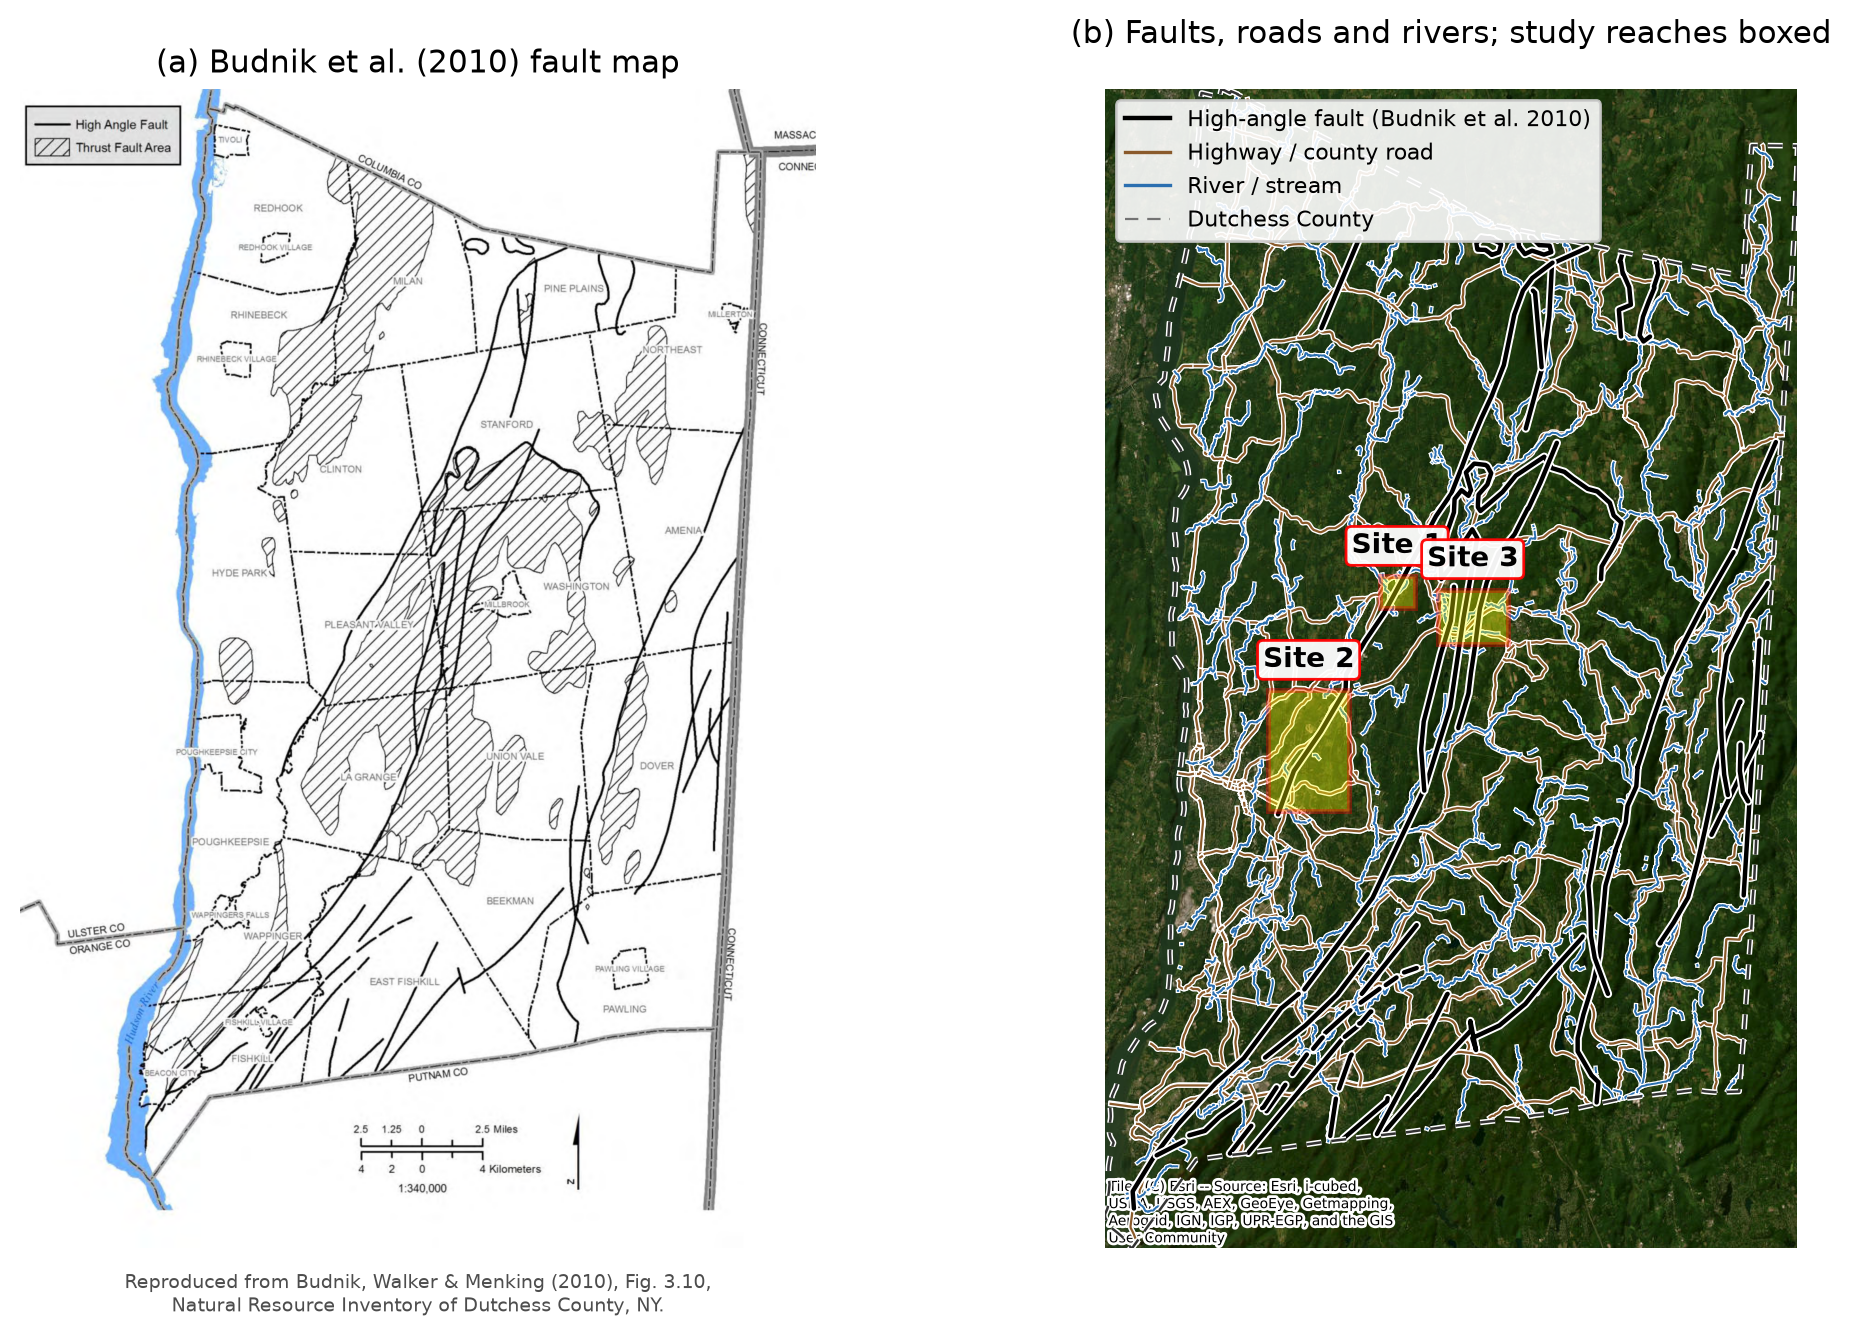
\includegraphics[width=\linewidth]{figures/overview.png}
%DIFDELCMD < 	%%%
\DIFdelendFL \DIFaddbeginFL 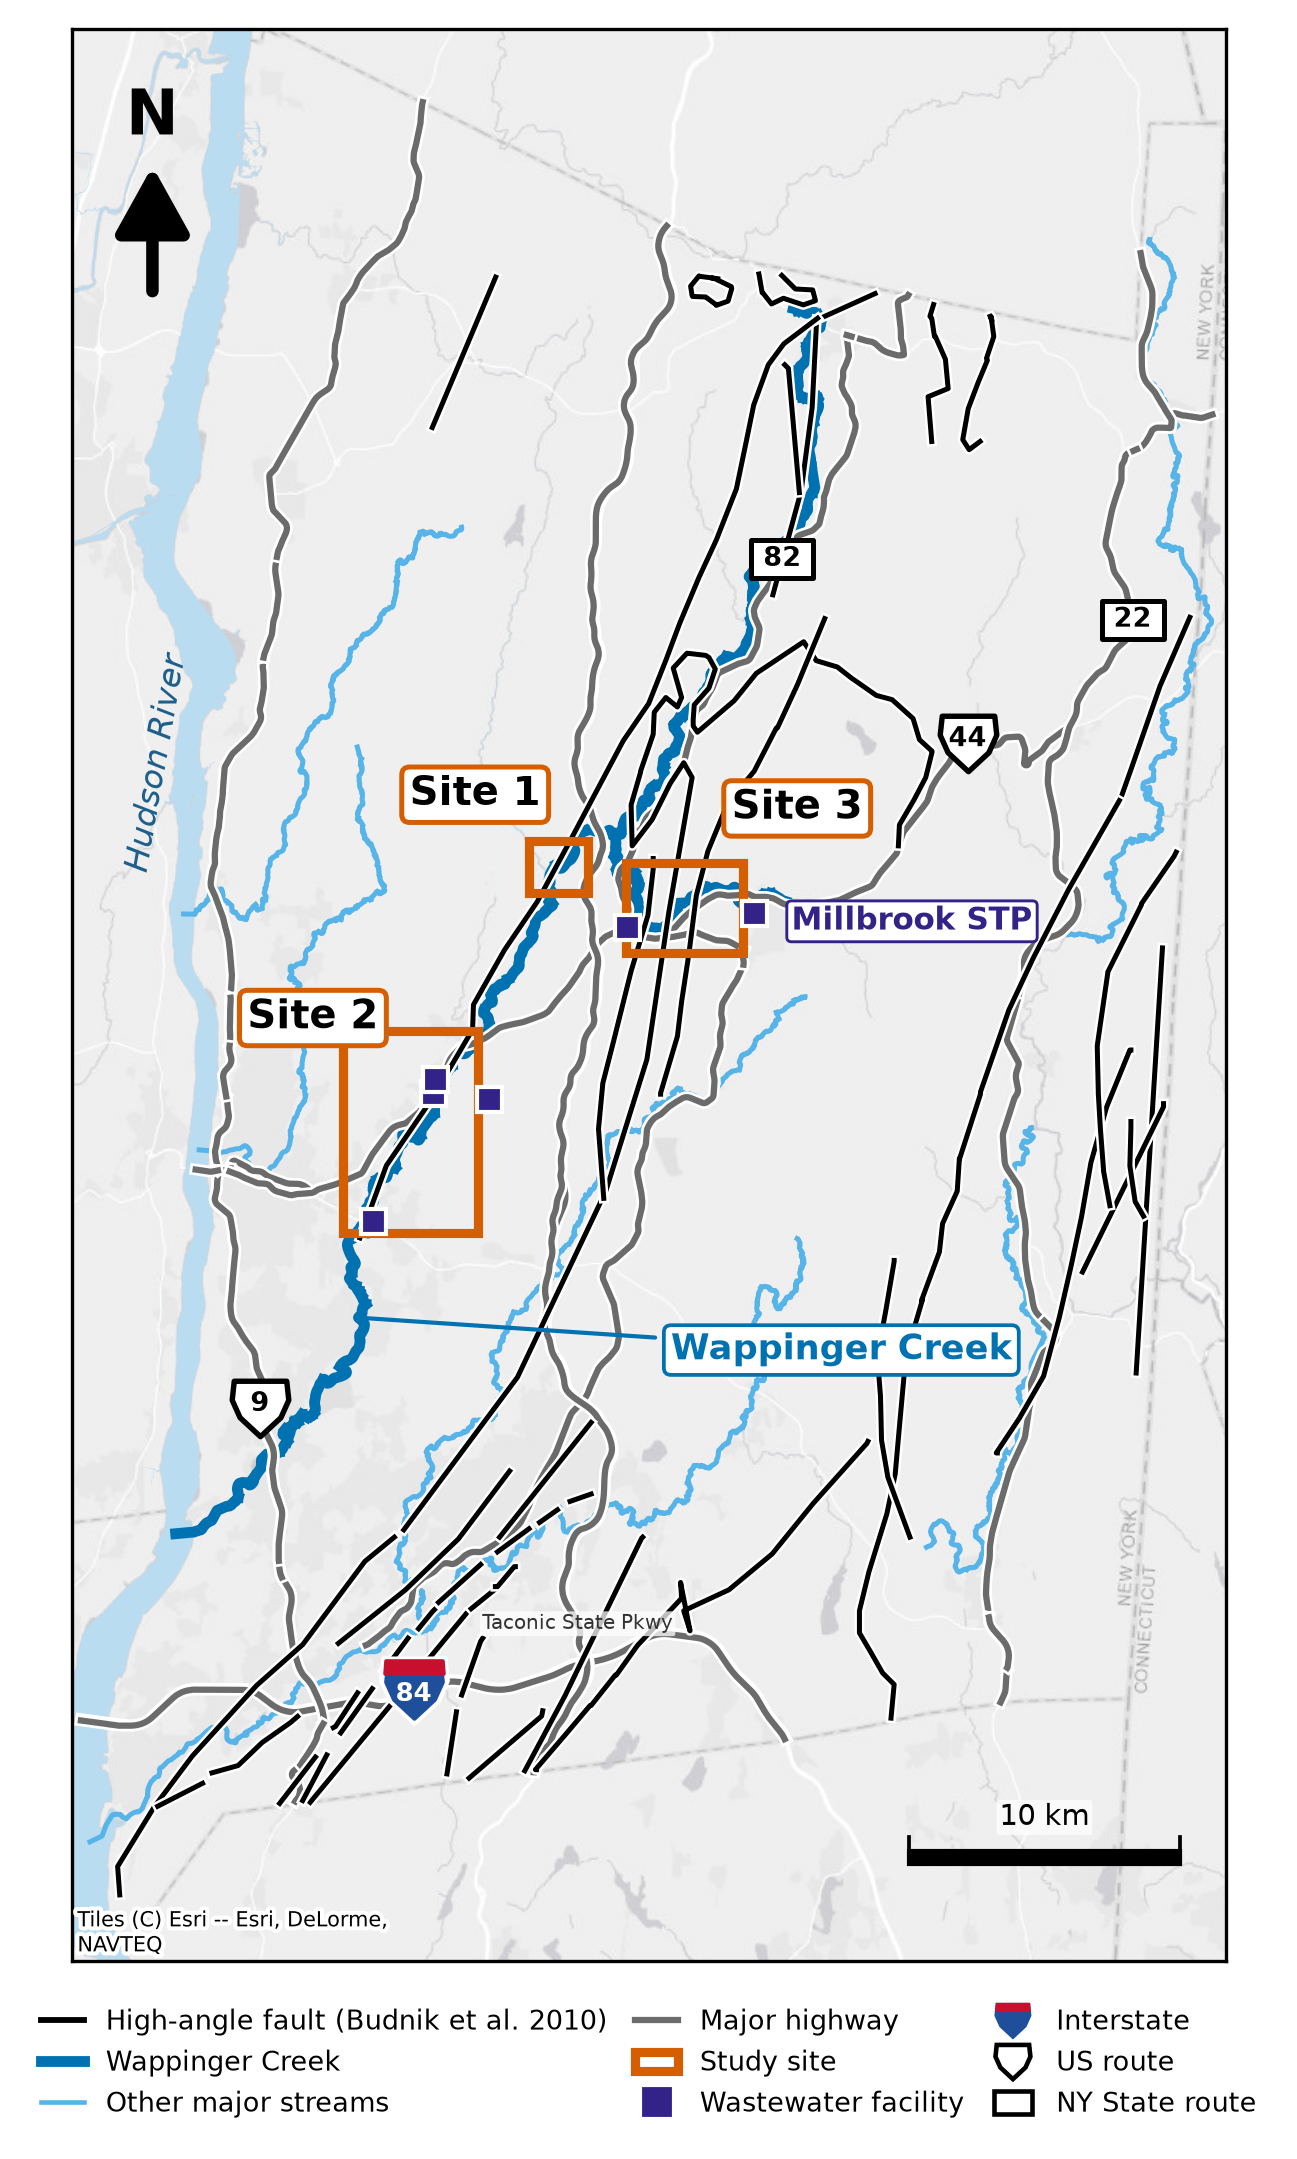
\includegraphics[width=\linewidth]{figures/rev_overview.png}
	\DIFaddendFL \caption{Study area\DIFdelbeginFL \DIFdelFL{overview}\DIFdelendFL . (a) \DIFdelbeginFL \DIFdelFL{The county fault map}\DIFdelendFL \DIFaddbeginFL \DIFaddFL{High-angle faults and thrust-fault areas in Dutchess County}\DIFaddendFL , \DIFdelbeginFL \DIFdelFL{taken directly }\DIFdelendFL \DIFaddbeginFL \DIFaddFL{reproduced }\DIFaddendFL from \citet{budnik2010}, Fig.~3.10\DIFdelbeginFL \DIFdelFL{, showing high-angle faults and thrust-fault areas across Dutchess County}\DIFdelendFL . (b) The three study reaches \DIFdelbeginFL \DIFdelFL{on Wappinger Creek }\DIFdelendFL (\DIFdelbeginFL \DIFdelFL{black }\DIFdelendFL \DIFaddbeginFL \DIFaddFL{orange }\DIFaddendFL boxes) on \DIFdelbeginFL \DIFdelFL{an OpenStreetMap base}\DIFdelendFL \DIFaddbeginFL \DIFaddFL{Wappinger Creek}\DIFaddendFL , with \DIFdelbeginFL \DIFdelFL{the same high-angle }\DIFdelendFL faults \DIFdelbeginFL \DIFdelFL{overlaid; each site sits where }\DIFdelendFL \DIFaddbeginFL \DIFaddFL{digitized from panel (}\DIFaddendFL a\DIFdelbeginFL \DIFdelFL{high-angle fault crosses the creek}\DIFdelendFL \DIFaddbeginFL \DIFaddFL{), wastewater facilities (squares) and major highways}\DIFaddendFL . \DIFdelbeginFL \DIFdelFL{Reach-scale conductivity for each site is detailed in Figures~\ref{fig:site1}--\ref{fig:site3}}\DIFdelendFL \DIFaddbeginFL \DIFaddFL{Sources: USGS NHD, US Census TIGER, EPA ECHO, Esri}\DIFaddendFL .}
	\label{fig:overview}
\end{figure}

\subsection{In-situ sampling}

\DIFaddbegin \linelabel{L:m-dates}\DIFaddend Conductivity measurements were \DIFdelbegin \DIFdel{obtained in October }\DIFdelend \DIFaddbegin \DIFadd{made on four days in autumn }\DIFaddend 2018\DIFdelbegin \DIFdel{; taking measurements approximately every hundred meters }\DIFdelend \DIFaddbegin \DIFadd{: Site 1 on 28 September, Site 2 on 5 October, and Site 3 on 19 and 26 October. The two Site 3 days correspond to three field surveys: one on 19 October (field site 3), and two on 26 October (field sites 4 and 5), which together repeat part of the 19 October reach. We measured from }\DIFaddend upstream to downstream\DIFaddbegin \DIFadd{, approximately every 100~m at Sites 1 and 3 and about every 400~m along the longer Site 2 reach, }\DIFaddend traversing either on foot inside or around the creek or floating along the channel. Sampling was performed in the thalweg of each study site\DIFdelbegin \DIFdel{using an electrical conductivity (EC) meter logging the specific conductance of the water, through which we inferred changes in levels of salt input to the stream along its length.
}%DIFDELCMD < 

%DIFDELCMD < %%%
\DIFdel{Performing measurements in the thalweg kept our data objective by reducing potential variations due to }\DIFdelend \DIFaddbegin \DIFadd{, which reduced variation due to incomplete }\DIFaddend lateral mixing. \DIFdelbegin \DIFdel{EC was converted to specific conductivity through adjusting the probe to 25 degrees Celsius. Measurements were taken using }\DIFdelend \DIFaddbegin \DIFadd{We used }\DIFaddend a Thermo Scientific Orion 013010MD \DIFdelbegin \DIFdel{Conductivity Cell calibrated using }\DIFdelend \DIFaddbegin \DIFadd{conductivity cell, calibrated following }\DIFaddend the standard protocols outlined by the manufacturer\DIFdelbegin \DIFdel{.
}\DIFdelend \DIFaddbegin \DIFadd{, with readings temperature-compensated to 25~$^{\circ}$C and reported as specific conductance. }\linelabel{L:m-accuracy}\DIFadd{The meters used with this cell specify an accuracy of $\pm$0.5\% of reading $\pm$1 digit, about $\pm$1.7~$\mu$S/cm at 310~$\mu$S/cm. A calibration offset shared by all readings on one day cancels when zones are compared within that day; random reading error does not.
We inferred changes in the salt input to the stream along its length from changes in specific conductance.
}\DIFaddend 

\DIFdelbegin \DIFdel{Each site was surveyed at a nominal spacing of roughly 100~m from upstream to downstream}\DIFdelend \DIFaddbegin \DIFadd{Mean spacing between points was about 85~m at Site 1}\DIFaddend , \DIFaddbegin \DIFadd{416~m at Site 2 and 83--118~m on the Site 3 surveys, }\DIFaddend yielding 9, 18, and 46 measurement points at Sites 1, 2, and 3, respectively, with point positions recorded using a handheld GPS unit. \DIFaddbegin \DIFadd{Along-channel distance for each survey was computed by summing great-circle distances between consecutive GPS fixes in survey order, with the surveys that were walked upstream reversed so that distance increases downstream. }\DIFaddend Within each site we delineated zones bounded at the locations where the creek crosses a mapped fault trace \DIFaddbegin \DIFadd{(at Site 2, the fault position interpreted in the field) }\DIFaddend or receives an active tributary, so that the reaches immediately upstream and downstream of a single geologic or hydrologic feature could be compared directly. To isolate the effect of faults, we restricted our fault-crossing contrasts to reaches where the creek intersects a mapped fault without a coincident tributary, because a tributary confluence introduces an independent salinity signal that would confound the comparison. Because the fault traces are mapped at county scale \DIFdelbegin \DIFdel{\mbox{%DIFAUXCMD
\citep{budnik2010}}\hskip0pt%DIFAUXCMD
, their horizontal positions carry an uncertainty of up to a few hundred meters; we therefore }\DIFdelend \DIFaddbegin \DIFadd{and are largely conjectural \mbox{%DIFAUXCMD
\citep{budnik2010}}\hskip0pt%DIFAUXCMD
, we }\DIFaddend treated each crossing as a reach-scale rather than a point-scale feature when assigning zone boundaries. \DIFaddbegin \DIFadd{Some survey points were flagged in the field log as lying just downstream of the mapped fault; the flag records what we believed at the time of sampling, not an observed fault position. }\DIFaddend Zones are numbered such that they ascend as the river goes downstream: for example zone 3-3 is downstream of 3-2 which is downstream of 3-1. \DIFdelbegin \DIFdel{Comparable dense spatial surveys of specific conductance and chloride have been used elsewhere to trace groundwater-sourced road salt to streams and springs, including in a karstic watershed where springs showed the strongest long-term increases \mbox{%DIFAUXCMD
\citep{orr2026}}\hskip0pt%DIFAUXCMD
. }\DIFdelend \DIFaddbegin \linelabel{L:site2-bend}\DIFadd{At Site 2 the digitized county-scale trace runs along the creek for the whole surveyed reach, so it cannot resolve where the fault crosses the channel. We placed the boundary between Zones 2-1 and 2-2 (Contrast B), about 4~km along the survey, at the position where we interpret the fault to be in the field: an abrupt, roughly 90$^{\circ}$ turn of the channel, which we took to be the creek turning to follow the fault and therefore a likely place of preferential groundwater flow along the structure. The boundary is thus a field interpretation of channel geometry, not a position taken from the mapped trace, whose locations are largely conjectural \mbox{%DIFAUXCMD
\citep{budnik2010}}\hskip0pt%DIFAUXCMD
. }\linelabel{L:site2-bend-caveat}\DIFadd{An abrupt bend is consistent with structural control of the channel, but it does not by itself show that groundwater flows along the fault there.
}\DIFaddend 

\DIFdelbegin \DIFdel{Chloride was assessed electronically using a calibrated YSI multi-probe during }\DIFdelend \DIFaddbegin \DIFadd{On 20 }\DIFaddend July 2020 \DIFdelbegin \DIFdel{within }\DIFdelend \DIFaddbegin \DIFadd{we measured chloride along a 2.35~km transect of the east fork at }\DIFaddend Site 3, \DIFdelbegin \DIFdel{upstream and downstream of }\DIFdelend \DIFaddbegin \DIFadd{from point Z (0~m) to point Z$'$ (2}{\DIFadd{,}}\DIFadd{351~m), passing }\DIFaddend the long-term monitoring \DIFdelbegin \DIFdel{location of \mbox{%DIFAUXCMD
\citet{kelly2019} }\hskip0pt%DIFAUXCMD
, }\DIFdelend \DIFaddbegin \DIFadd{site of \mbox{%DIFAUXCMD
\citet{kelly2019} }\hskip0pt%DIFAUXCMD
at about 1}{\DIFadd{,}}\DIFadd{224~m (Figure~\ref{fig:chloride}). The aim was to see whether chloride rose near the mapped faults. We took 18 samples in the main channel and one in a side tributary. }\linelabel{L:cl-sensor}\DIFadd{Chloride was measured with a calibrated YSI Pro Series 1005 chloride ion-selective electrode (YSI 605105) on a YSI handheld meter. }\linelabel{L:cl-accuracy}\DIFadd{The manufacturer gives an accuracy of $\pm$15\% of reading or $\pm$5~mg/L, whichever is greater, which at our concentrations (about 14--50~mg/L) is $\pm$5 }\DIFaddend to \DIFdelbegin \DIFdel{determine whether rises in chloride concentration occurred close to the mapped geologic faults. This longitudinal chloride transect spanned roughly one kilometer of the east fork, expressed as relative distance from an upstream point Z to a downstream point Z' (Figure~\ref{fig:chloride}) , and was collected in summer, when the stream is at baseflowand any }\DIFdelend \DIFaddbegin \DIFadd{$\pm$7.5~mg/L, so differences of a few mg/L between neighboring samples are within instrument error.
}

\DIFadd{The transect was sampled in midsummer, when streamflow is likely dominated by baseflow, so }\DIFaddend elevated chloride is more plausibly \DIFdelbegin \DIFdel{attributed to groundwater than to concurrent road-salt runoff. Sampling in July, nearly two years after the October 2018 }\DIFdelend \DIFaddbegin \DIFadd{from groundwater than from runoff. }\linelabel{L:cl-single}\DIFadd{Because it is a single transect from a different year than the }\DIFaddend conductivity survey, \DIFdelbegin \DIFdel{also provided an independent test of whether the same spatial patternrecurred across years and across a second, more salt-specific measurement.
}\DIFdelend \DIFaddbegin \DIFadd{it cannot confirm the conductivity pattern; we describe it and apply the same change-point method used for conductance.
}\DIFaddend 

\subsection{Statistical analysis}
\DIFaddbegin \label{sec:stats}
\DIFaddend 

\DIFdelbegin \DIFdel{The specific conductance was normalized within each site using mean/standard-deviation (z-score) normalization (Equation~\ref{eq:normalization}), with the sample mean $\overline{X}$ and sample standard deviation $\sigma_x$ computed separately for each site.
This removes day-to-day differences in the overall conductivity level and streamflow between sampling dates and places all sites on a common, dimensionless scale so that the relative rise or fall across a feature can be compared regardless of a site's absolute salinity.
}%DIFDELCMD < 

%DIFDELCMD < %%%
\begin{displaymath}
	\DIFdel{\mu_{0} = \frac{x - \overline{X}}{\sigma_{x}}
	%DIFDELCMD < \label{eq:normalization}%%%
}\end{displaymath}%DIFAUXCMD
%DIFDELCMD < 

%DIFDELCMD < %%%
\DIFdel{Next, we }\DIFdelend \DIFaddbegin \DIFadd{We }\DIFaddend separated the specific-conductance samples into zones defined by where geologic interactions occur, that is, where the stream crosses either a fault or a side-stream. \DIFaddbegin \linelabel{L:m-welch}\DIFaddend We then applied a two-sample Welch $t$-test (Equation~\ref{eq:ttest}) to evaluate the difference in mean specific conductance\DIFaddbegin \DIFadd{, in $\mu$S/cm, }\DIFaddend upstream and downstream of each feature. Unlike Student's pooled $t$-test, Welch's version does not assume equal variances \DIFdelbegin \DIFdel{between the two zones, and it remains reliable when the groups have both unequal variances and unequal }\DIFdelend \DIFaddbegin \DIFadd{and remains reliable with unequal }\DIFaddend sample sizes, as ours \DIFdelbegin \DIFdel{do; for these reasons it }\DIFdelend \DIFaddbegin \DIFadd{are, and }\DIFaddend is recommended as the default two-sample test \citep{ruxton2006}.

\begin{equation}
	t = \frac{\overline{x}_{2} - \overline{x}_{1}}{\sqrt{\dfrac{s_{1}^{2}}{n_{1}} + \dfrac{s_{2}^{2}}{n_{2}}}}
	\label{eq:ttest}
\end{equation}

Here $\overline{x}_{1}$ and $\overline{x}_{2}$ are the mean specific conductance of the upstream and downstream zones, $s_{1}$ and $s_{2}$ their standard deviations, and $n_{1}$ and $n_{2}$ their sample sizes. \DIFdelbegin \DIFdel{Applying a $t$-test to measurements collected sequentially along a channel warrants caution, because closely spaced samples are not strictly independent. We treated the measurements within a zone as approximate replicates of that reach's ambient salinity and tested only the difference in means between adjacent zones; because the within-zone scatter is small relative to the between-zone contrasts (Table~\ref{tab:ttest}), we interpret a significant contrast as a genuine step change across the intervening feature rather than an artifact of fine-scale autocorrelation. Site 3 was surveyed over two daysowing to its length, but every zone-to-zone contrast was computed within a single day 's data, and the per-site normalization (Equation~\ref{eq:normalization}) removes any offsetin baseline conductivity between the two days, so the comparisons remain valid}\DIFdelend \DIFaddbegin \linelabel{L:m-withinday}\DIFadd{Zones are compared only within a single survey day. Synoptic comparisons along a stream assume steady conditions, because concentrations that change between sampling runs are a source of uncertainty in a longitudinal profile \mbox{%DIFAUXCMD
\citep{runkel2013}}\hskip0pt%DIFAUXCMD
. }\linelabel{L:m-offset}\DIFadd{At Site 3 the two survey days differ by a consistent offset: eleven pairs of 19 and 26 October points lying within 120~m of one another differ by 23.5 to 29.7~$\mu$S/cm (mean 27.8~$\mu$S/cm), larger than any of the contrasts we test. We did not pool days, add a day covariate, or correct for the offset. Contrast D is therefore tested on 19 October, and Contrast E on 26 October}\DIFaddend . We evaluated significance with two-tailed tests at $\alpha = 0.05$. Because our zone samples are \DIFdelbegin \DIFdel{realtively small in size }\DIFdelend \DIFaddbegin \DIFadd{relatively small }\DIFaddend and not guaranteed to be normally distributed, we accompanied every Welch test with a distribution-free Mann--Whitney $U$ test and regard a contrast as robust only where the two approaches agree, which guards against over-interpreting the smaller contrasts.

\DIFaddbegin \linelabel{L:m-autocorr}\DIFadd{Applying a $t$-test to measurements collected sequentially along a channel warrants caution, because closely spaced samples are not strictly independent and nominal $p$-values are therefore likely too small. For each contrast we estimated the lag-1 autocorrelation $\rho$ of the residuals from the two zone means, pooled in along-channel order. Negative values were set to zero and $\rho$ was capped at 0.9. We then computed an effective sample size for each zone, $n_{\mathrm{eff}} = n(1-\rho)/(1+\rho)$, floored at 2 and not exceeding $n$, and repeated the Welch test with $n_{\mathrm{eff}}$ in place of $n$ (degrees of freedom by the Welch--Satterthwaite approximation). }\linelabel{L:m-autocorr-check}\DIFadd{With zones of three to eleven points, $\rho$ is poorly determined, so we treat the adjusted $p$-values as a sensitivity check rather than a correction.
}

\linelabel{L:m-changepoint}\DIFadd{Zone means cannot show whether a change in conductance is abrupt or gradual, so we also looked for change points along each transect. For each single-day transect separately (Site 1, Site 2, the 19 October survey at Site 3, and the upper and lower 26 October surveys at Site 3), we fitted continuous piecewise-linear regressions of specific conductance on along-channel distance with zero, one, or two breakpoints, requiring at least three points in each segment, and chose the number of breakpoints by the Bayesian information criterion (BIC). Uncertainty in each breakpoint was assessed with a residual bootstrap (500 replicates). As an independent check we applied a penalized change-in-mean analysis (PELT, }\texttt{\DIFadd{ruptures}} \DIFadd{package). The same procedure was applied to the chloride transect.
}

\DIFadd{Finally, because roads are a possible alternative source of the conductance differences, we computed the distance from each survey point to the nearest major road, defined as primary or secondary roads (TIGER/Line 2024 feature classes S1100 and S1200). We report these distances descriptively by zone and do not test them.
}

\DIFaddend \section{Results}

\DIFdelbegin \subsection{\DIFdel{Contrasts}}
%DIFAUXCMD
\addtocounter{subsection}{-1}%DIFAUXCMD
\DIFdelend \DIFaddbegin \subsection{\DIFadd{Within-day zone contrasts}}
\DIFaddend 

\DIFdelbegin \DIFdel{Site 1 was split into two zones (}\DIFdelend \DIFaddbegin \DIFadd{Zones are compared only within a single survey day, so the results are reported survey by survey. }\linelabel{L:table-intro}\DIFadd{Table~\ref{tab:ttest} gives each contrast with zone means $\pm$ SD and the number of points $n$; Table~\ref{tab:support} gives the autocorrelation-adjusted $p$-values and the median distance from each zone's points to the nearest major road; Appendix~A lists every measurement. }\linelabel{L:sd-range}\DIFadd{Within a single day the zone standard deviations are 0.1--2.6~$\mu$S/cm.
}

\textbf{\DIFadd{Site 1, Contrast A (28 September).}} \DIFadd{Specific conductance fell from 259.9 $\pm$ 0.7~$\mu$S/cm in }\DIFaddend Zone \DIFdelbegin \DIFdel{1-1 and Zone 1-2), with a single contrast (Contrast A)used for analysis where Wappinger Creek abruptly veers along the mapped fault trace (Figure~\ref{fig:site1}). Before the fault interaction, the sample-mean specific conductance for Zone }\DIFdelend 1-1 \DIFdelbegin \DIFdel{was 259.9}\DIFdelend \DIFaddbegin \DIFadd{($n = 4$) to 259.4 $\pm$ 0.1}\DIFaddend ~$\mu$S/cm \DIFdelbegin \DIFdel{; after the fault, at }\DIFdelend \DIFaddbegin \DIFadd{in }\DIFaddend Zone 1-2 \DIFdelbegin \DIFdel{, it decreased slightly to 259.4}\DIFdelend \DIFaddbegin \DIFadd{($n = 5$), a change of $-0.5$}\DIFaddend ~$\mu$S/cm \DIFdelbegin \DIFdel{. This slight decrease across the fault, however, coincided with an active tributary entering the creek }\DIFdelend \DIFaddbegin \DIFadd{that is not significant (Figure~\ref{fig:site1}; Table~\ref{tab:ttest}). A tributary enters }\DIFaddend at the same \DIFdelbegin \DIFdel{location, so the contrast at Site 1 cannot be attributed to the fault alone. Site 1 is instructive nonetheless: the channel veers to follow }\DIFdelend \DIFaddbegin \DIFadd{place where the channel turns along }\DIFaddend the mapped fault trace\DIFdelbegin \DIFdel{(Figure~\ref{fig:site1}), precisely the geometry in which a fault-conduit signal might be expected to appear, but the coincident tributary, together with a rain event during sampling that lowered specific conductance across this reach by }\DIFdelend \DIFaddbegin \DIFadd{, and the field log records very high flow after rain throughout the Site 1 survey; conductance there was }\DIFaddend 50--100~$\mu$S/cm \DIFdelbegin \DIFdel{relative to the other two sites, makes this crossing unsuitable for isolating the fault . We therefore exclude Contrast A from the set of clean fault crossings.
}\DIFdelend \DIFaddbegin \DIFadd{lower than at the other sites, consistent with dilution by runoff, so this contrast cannot isolate a fault effect and, with four and five points, has little power.
}\DIFaddend 

\begin{figure}[htbp]
	\centering
	\DIFdelbeginFL %DIFDELCMD < 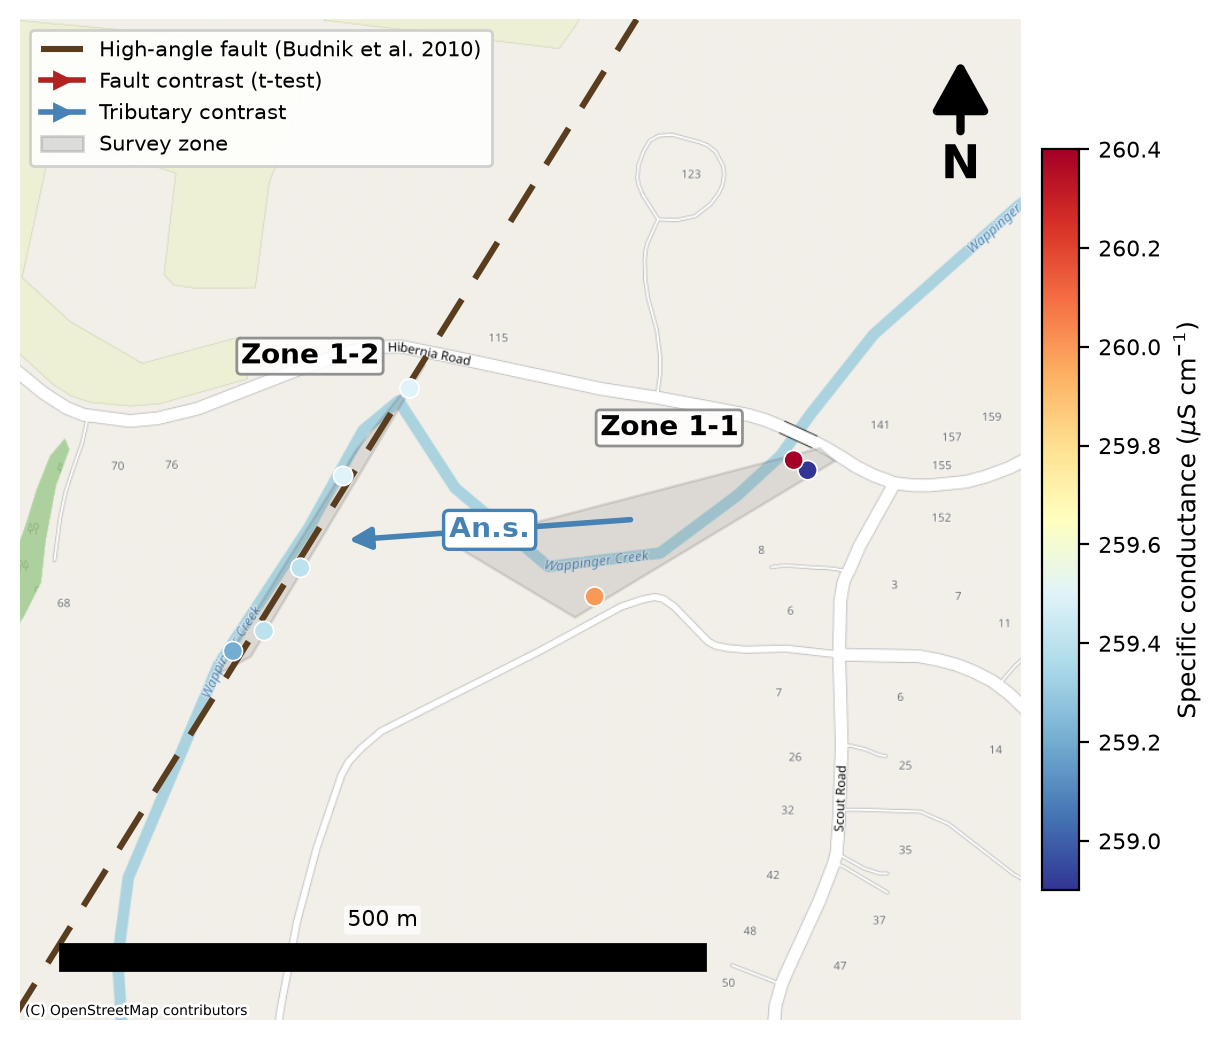
\includegraphics[width=0.62\linewidth]{figures/site1.png}
%DIFDELCMD < 	%%%
\DIFdelendFL \DIFaddbeginFL 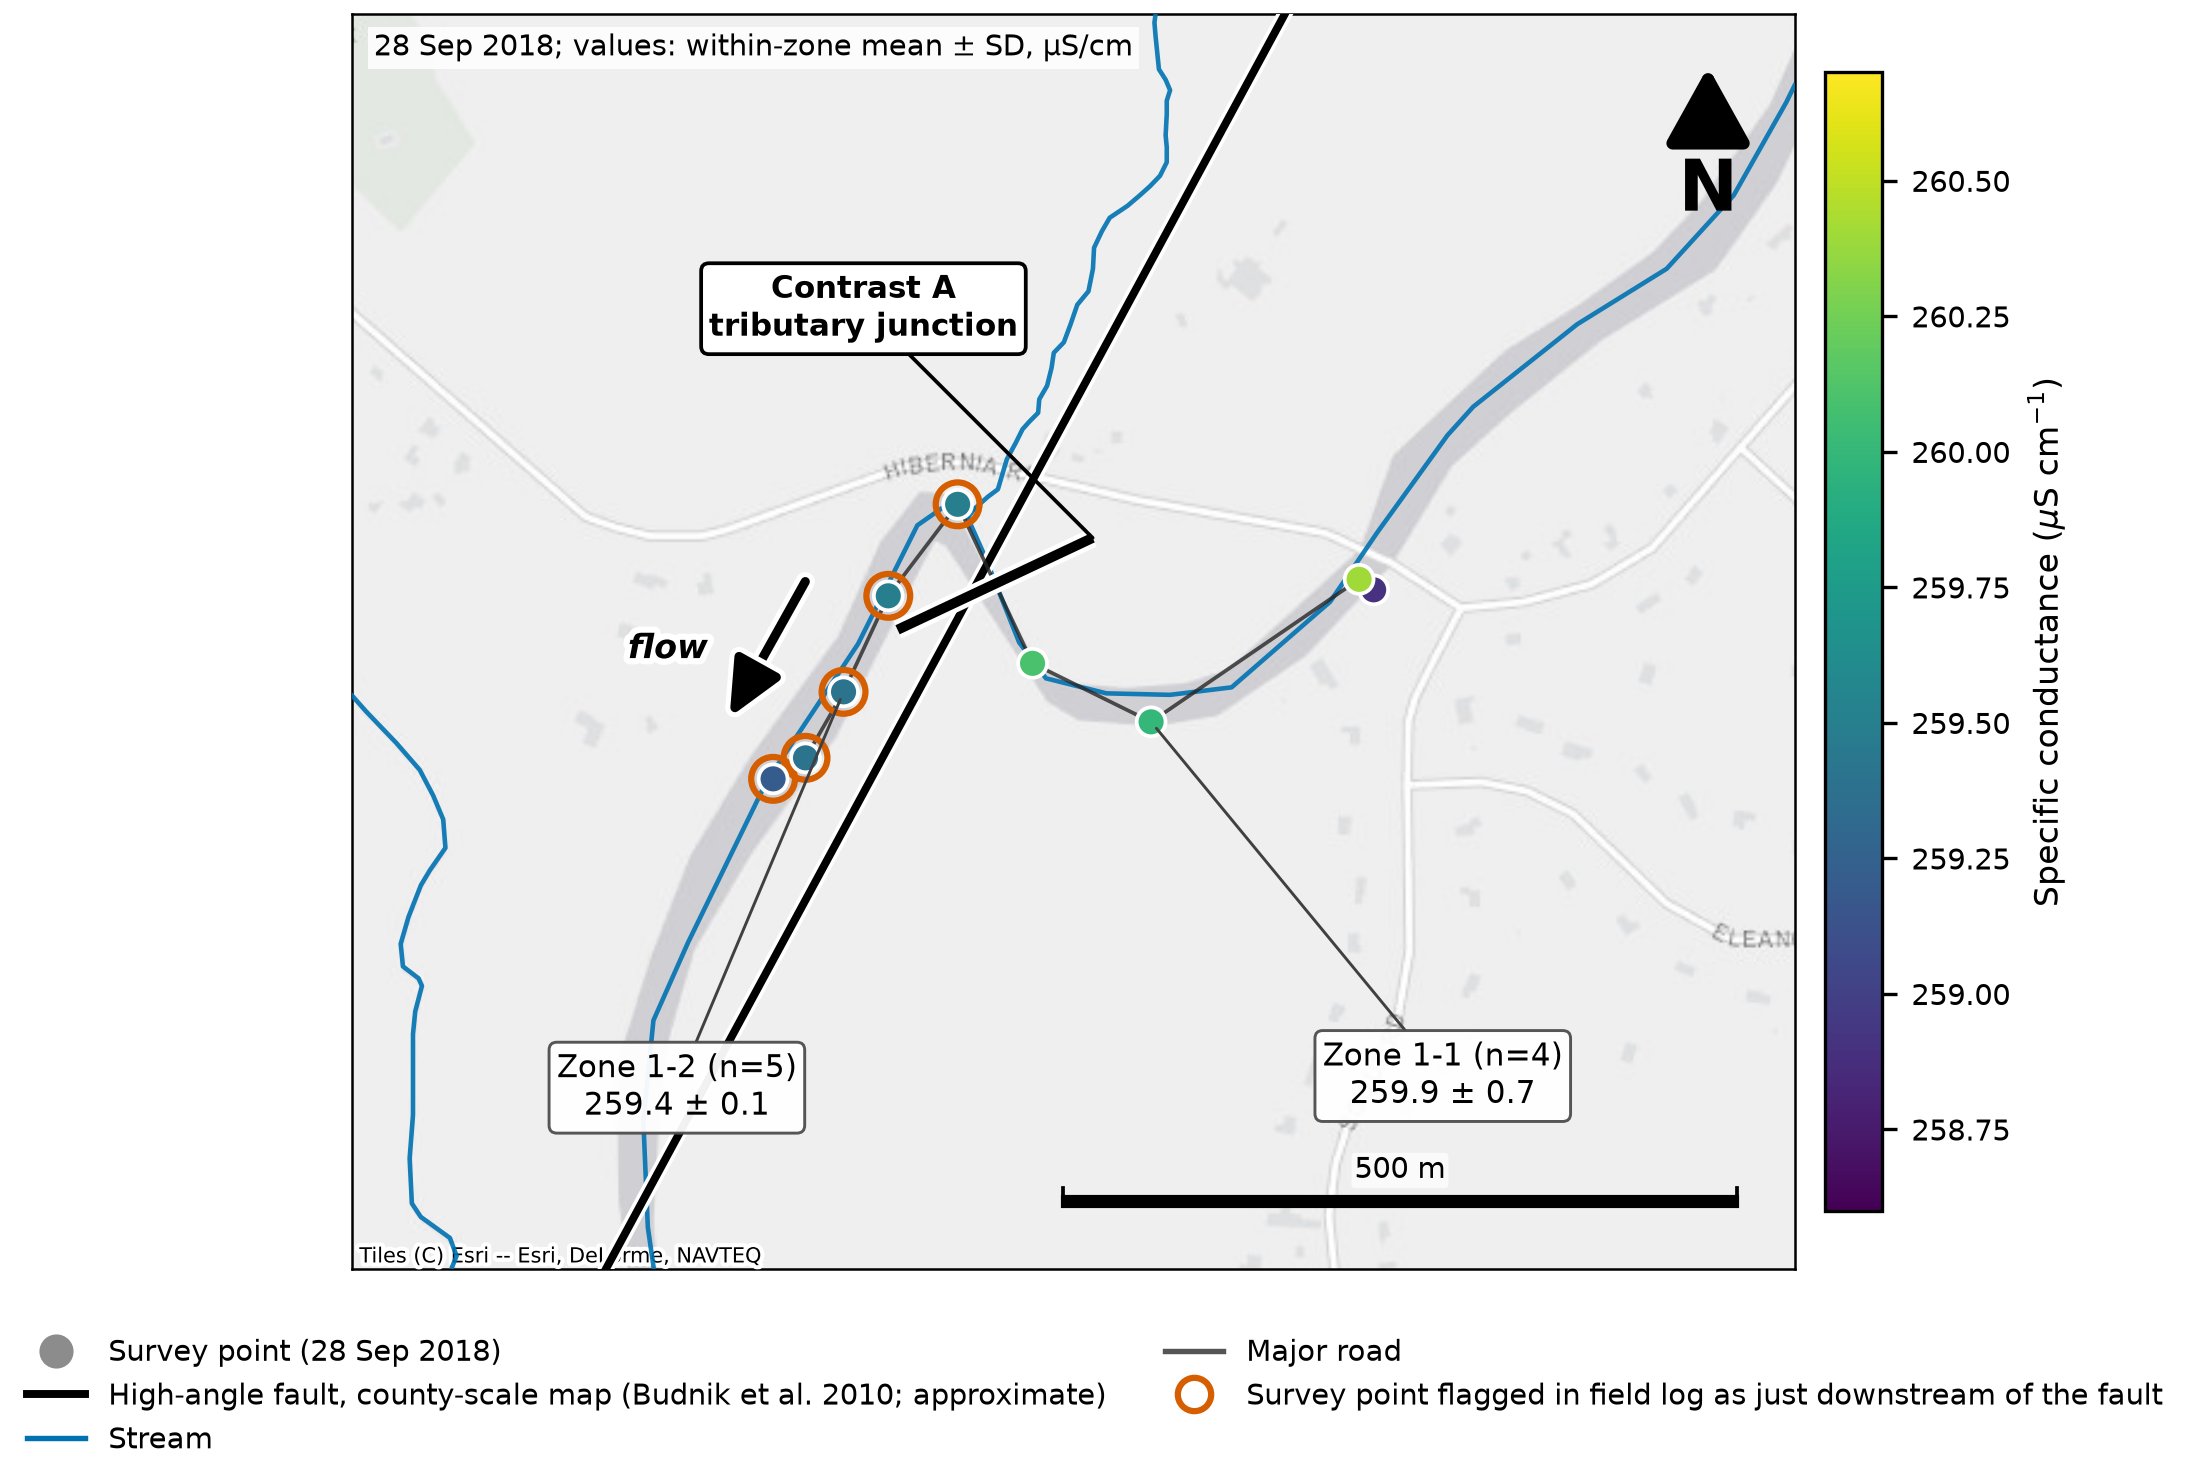
\includegraphics[width=0.7\linewidth]{figures/rev_site1.png}
	\DIFaddendFL \caption{Site 1 \DIFdelbeginFL \DIFdelFL{on a terrain base with highways/county roads }\DIFdelendFL (\DIFdelbeginFL \DIFdelFL{brown}\DIFdelendFL \DIFaddbeginFL \DIFaddFL{28 September 2018}\DIFaddendFL ) and \DIFdelbeginFL \DIFdelFL{streams (blue)}\DIFdelendFL \DIFaddbeginFL \DIFaddFL{Contrast A}\DIFaddendFL . \DIFdelbeginFL \DIFdelFL{Survey points }\DIFdelendFL \DIFaddbeginFL \DIFaddFL{Points }\DIFaddendFL are coloured by specific conductance; \DIFdelbeginFL \DIFdelFL{red-outlined regions are }\DIFdelendFL \DIFaddbeginFL \DIFaddFL{orange rings mark points logged as just downstream of }\DIFaddendFL the \DIFdelbeginFL \DIFdelFL{survey zones, labelled with their mean specific conductance}\DIFdelendFL \DIFaddbeginFL \DIFaddFL{fault}\DIFaddendFL . \DIFdelbeginFL \DIFdelFL{Zones are numbered in ascending order downstream (}\DIFdelendFL Zone \DIFdelbeginFL \DIFdelFL{1-1 upstream, 1-2 downstream). High-angle faults }\DIFdelendFL \DIFaddbeginFL \DIFaddFL{labels give $n$ and mean $\pm$ SD }\DIFaddendFL (\DIFdelbeginFL \DIFdelFL{thick black lines}\DIFdelendFL \DIFaddbeginFL \DIFaddFL{$\mu$S/cm}\DIFaddendFL )\DIFdelbeginFL \DIFdelFL{are approximate, digitized }\DIFdelendFL \DIFaddbeginFL \DIFaddFL{. Faults }\DIFaddendFL from \citet{budnik2010}.\DIFdelbeginFL \DIFdelFL{Statistical comparisons between zones are given in Table~\ref{tab:ttest}.}\DIFdelendFL }
	\label{fig:site1}
\end{figure}

\DIFdelbegin \DIFdel{Site 2 (Figure~\ref{fig:site2}) has one contrast (Contrast B) between two zones (Zones 2-1 and 2-2). Wappinger Creek parallels a fault line, turns river right due to the topography, then sharply shoots river left at the fault line. }\DIFdelend \DIFaddbegin \textbf{\DIFadd{Site 2, Contrast B (5 October).}} \DIFaddend Zone 2-1 \DIFdelbegin \DIFdel{contained a mean specific conductance level of }\DIFdelend \DIFaddbegin \DIFadd{averaged }\DIFaddend 308.8 \DIFdelbegin \DIFdel{~}\DIFdelend \DIFaddbegin \DIFadd{$\pm$ 1.1~}\DIFaddend $\mu$S/\DIFdelbegin \DIFdel{cm, while Zone }\DIFdelend \DIFaddbegin \DIFadd{cm ($n = 10$) and Zone }\DIFaddend 2-2 \DIFdelbegin \DIFdel{had a value of }\DIFdelend \DIFaddbegin \DIFadd{averaged }\DIFaddend 313.1 \DIFaddbegin \DIFadd{$\pm$ 1.9}\DIFaddend ~$\mu$S/\DIFaddbegin \DIFadd{cm ($n = 8$), an increase of $+4.3$~$\mu$S/cm (95\% CI $+2.6$ to $+6.0$; Welch $p < 0.001$; Mann--Whitney $p < 0.001$; Figure~\ref{fig:site2}). }\linelabel{L:contrastB-adj}\DIFadd{Allowing for autocorrelation along the channel ($n_{\mathrm{eff}} = 4.6$ and 3.7), the adjusted $p$ is 0.017 (Table~\ref{tab:support}). The difference is larger than the within-zone standard deviations and about 2.5 times the instrument's stated accuracy at this conductance ($\pm$1.7~$\mu$S/}\DIFaddend cm \DIFdelbegin \DIFdel{. This increase indicates the creek increased in conductivity after the fault line intersection. Site 2 offers the cleanest geometry of the three: the creek runs parallel to a single mapped fault and then crosses it with no tributary entering the reach, so Contrast B provides the most direct test of the fault-conduit hypothesis.
Although the mean increase across the crossing is modest at 4.3}\DIFdelend \DIFaddbegin \DIFadd{at 310}\DIFaddend ~$\mu$S/cm\DIFdelbegin \DIFdel{, the within-zone scatter is small enough that the rise is highly significant (Table~\ref{tab:ttest}) .
}\DIFdelend \DIFaddbegin \DIFadd{). The Zone 2-1/2-2 boundary, about 4.0~km along the survey, is the fault position we interpreted in the field from the abrupt 90$^{\circ}$ channel bend (Section~2.2). }\linelabel{L:site2-trace}\DIFadd{The digitized county-scale trace runs along the creek throughout and crosses the survey line at about 1.0 and 5.8~km, but those intersections are not reliable fault positions, so we did not use them. }\linelabel{L:site2-flow}\DIFadd{The field log records very high flow at the start of the Site 2 survey, part of which was made by canoe, so this survey may not represent baseflow.
}\DIFaddend 

\begin{figure}[htbp]
	\centering
	\DIFdelbeginFL %DIFDELCMD < 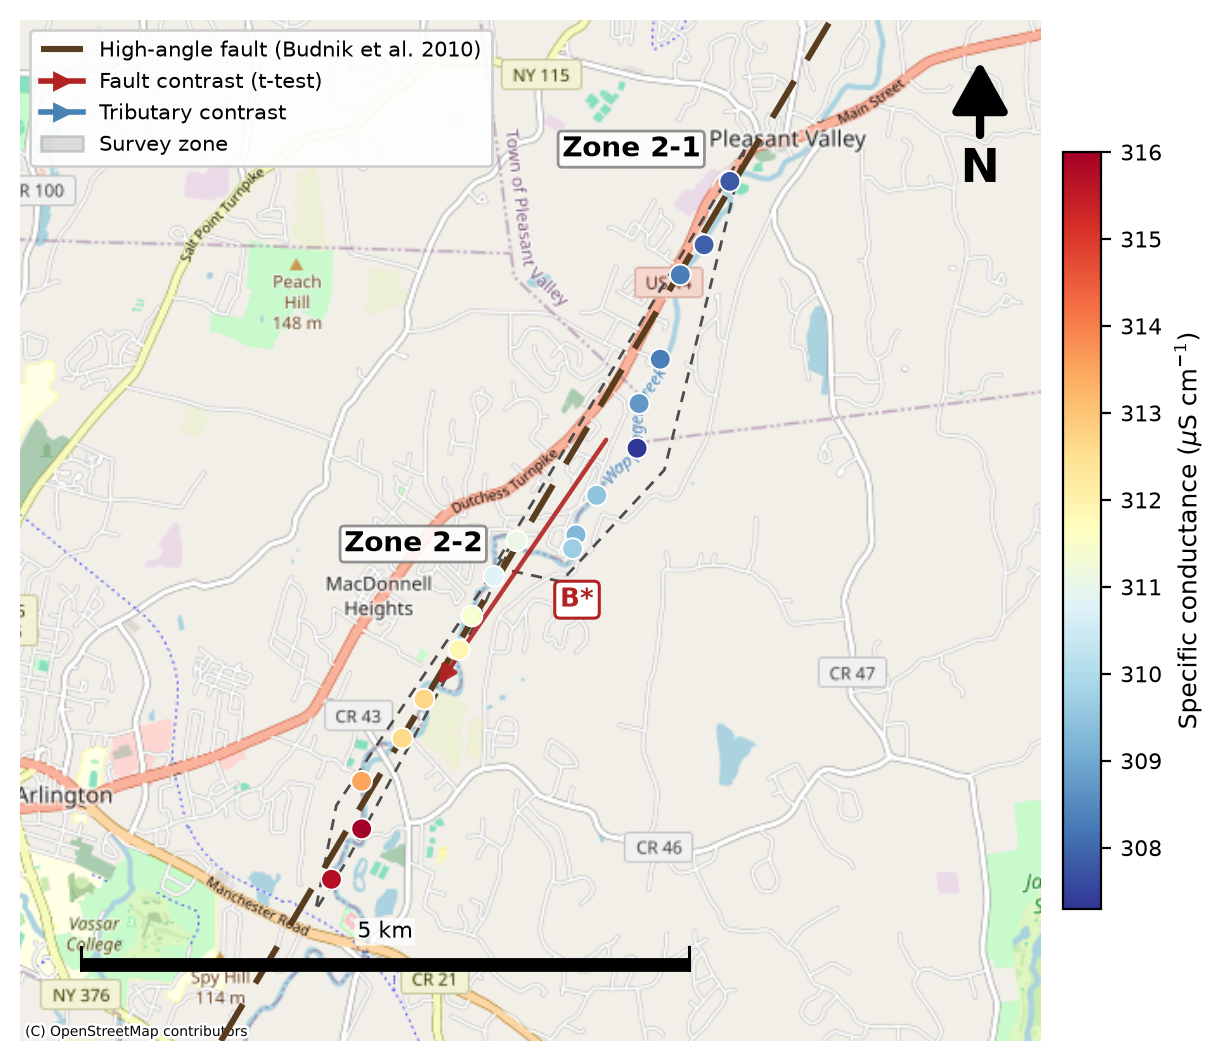
\includegraphics[width=0.52\linewidth]{figures/site2.png}
%DIFDELCMD < 	%%%
%DIFDELCMD < \caption{%
{%DIFAUXCMD
\DIFdelFL{Site 2, symbolised as in Figure~\ref{fig:site1}: terrain base, roads (brown) and streams (blue), survey points coloured by specific conductance, and red-outlined survey zones labelled with their mean specific conductance. Zones are numbered in ascending order downstream. High-angle faults (thick black) are approximate, digitized from \mbox{%DIFAUXCMD
\citet{budnik2010}}\hskip0pt%DIFAUXCMD
. Statistical comparisons between zones are given in Table~\ref{tab:ttest}.}}
	%DIFAUXCMD
\DIFdelendFL \DIFaddbeginFL 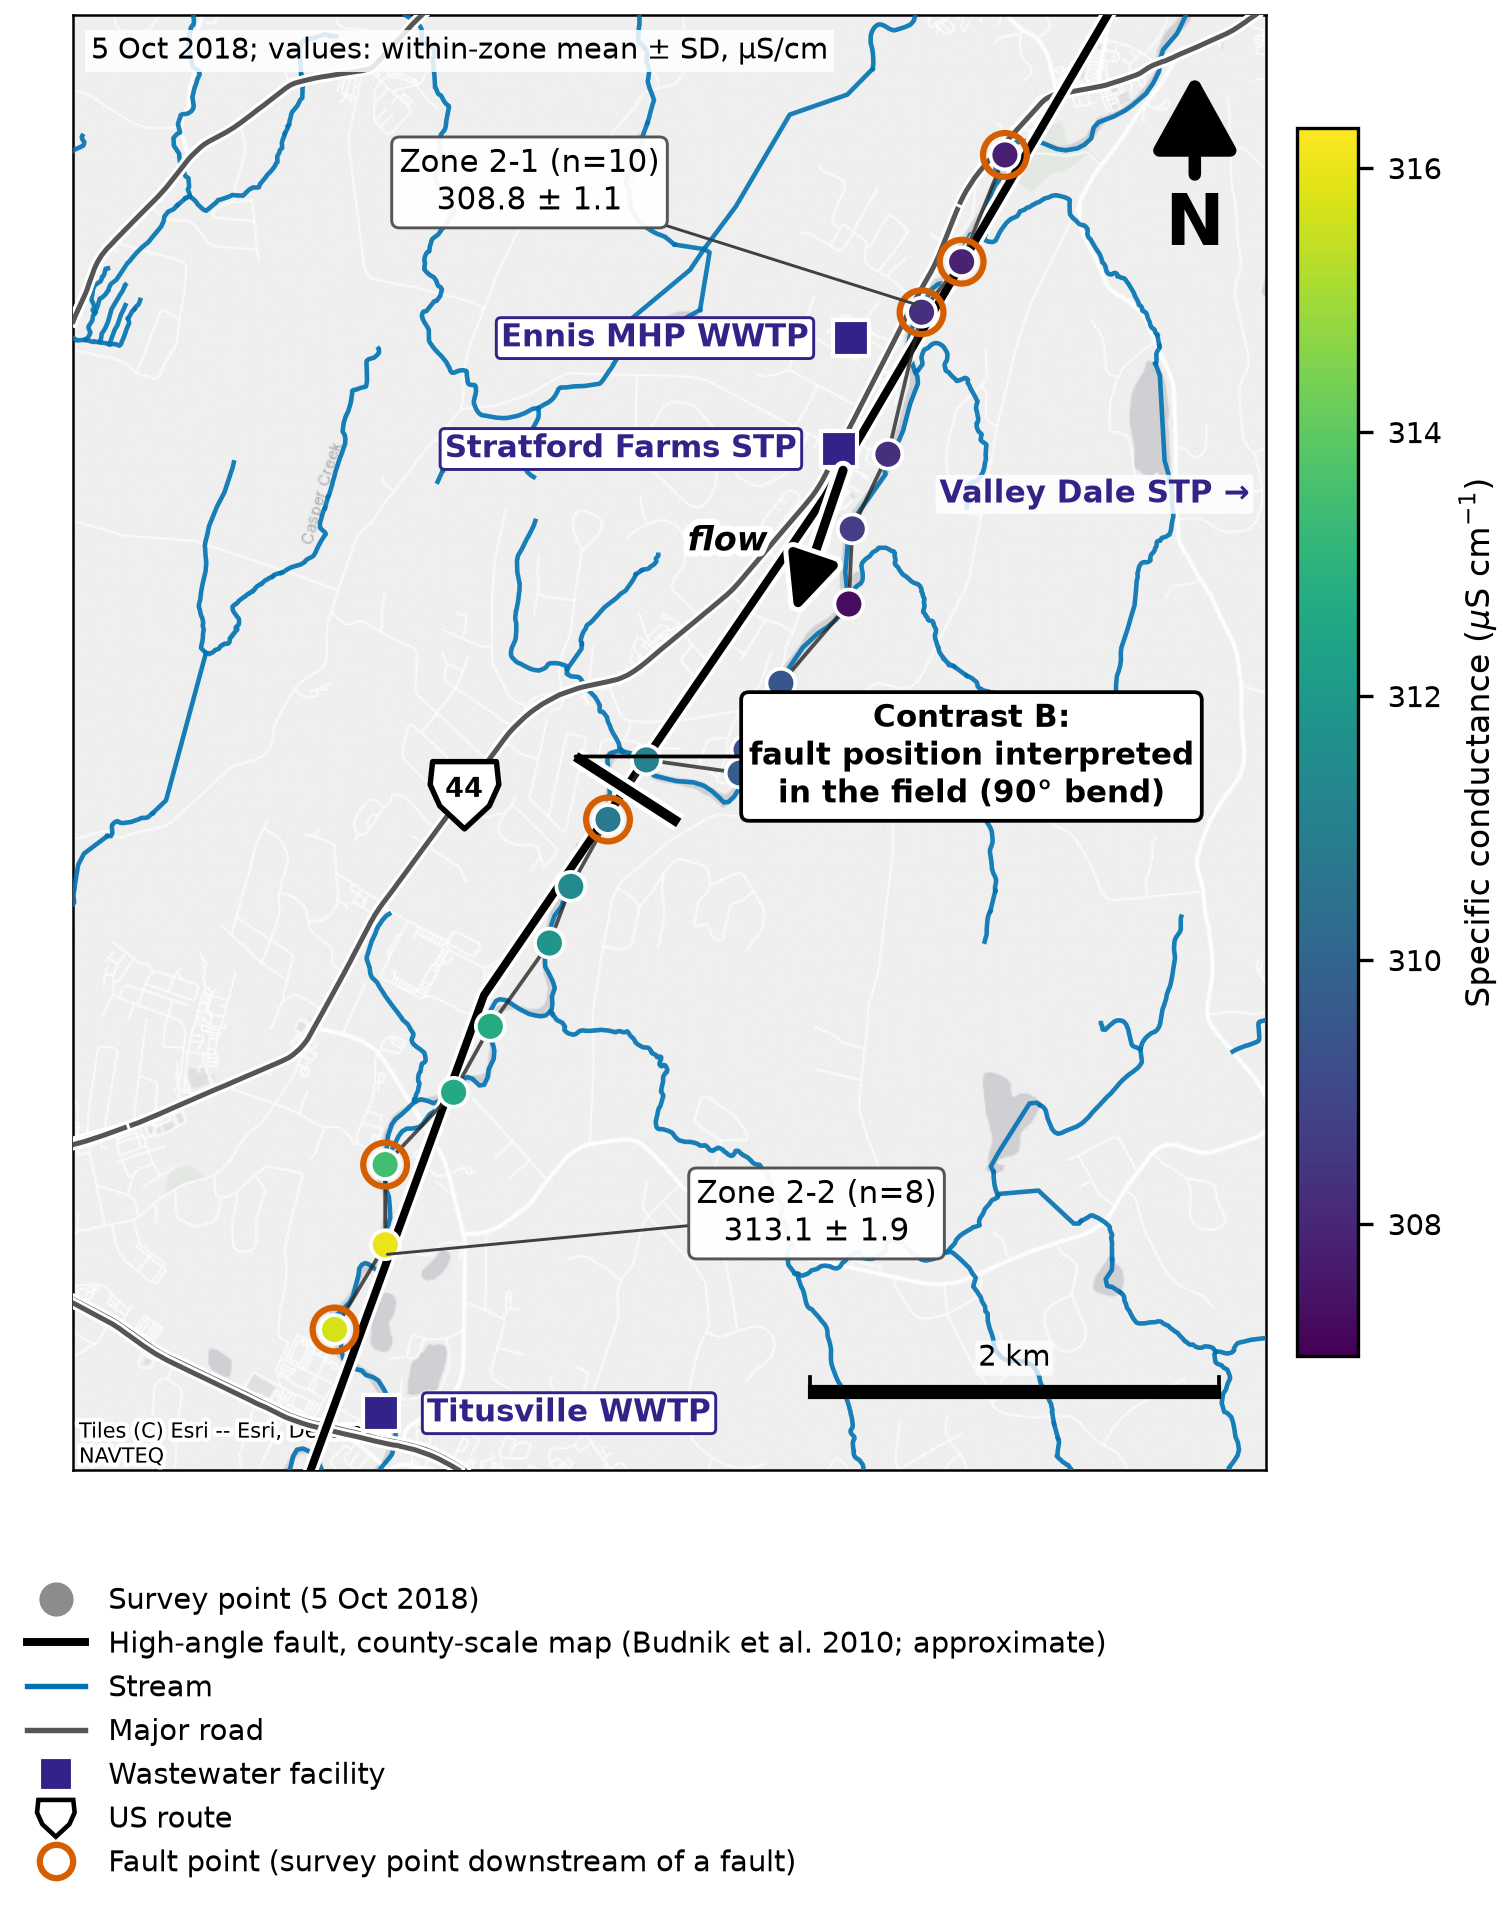
\includegraphics[width=0.78\linewidth]{figures/rev_site2.png}
	\caption{\DIFaddFL{Site 2 (5 October 2018) and Contrast B. Symbols as in Figure~\ref{fig:site1}. The zone boundary is the fault position interpreted in the field at an abrupt 90$^{\circ}$ bend; squares are wastewater facilities.}}
	\DIFaddendFL \label{fig:site2}
\end{figure}

\DIFdelbegin \DIFdel{Site 3 (Figure~\ref{fig:site3}) contains four zones (Zones 3-1, 3-2, 3-3, and 3-4)}\DIFdelend \DIFaddbegin \textbf{\DIFadd{Site 3, Contrasts C, D and E (19 and 26 October).}} \DIFadd{Contrast C, the tributary junction, is a decrease on both days: $-3.8$~$\mu$S/cm on 19 October (340.1 $\pm$ 0.4}\DIFaddend , \DIFdelbegin \DIFdel{with the zone transitions corresponding to a side stream (Contrast C) and two faults (Contrast D and E). The east fork of Wappinger Creek intersects a small side stream, turns river left at a faultintersection, then wraps around a hill and darts river left along a second fault line. Zones 3-1 }\DIFdelend \DIFaddbegin \DIFadd{$n = 6$, to 336.3 $\pm$ 2.2, $n = 3$; Welch $p = 0.093$; Mann--Whitney $p = 0.028$) }\DIFaddend and \DIFdelbegin \DIFdel{3-2 yielded mean specific conductance levels of 359.8 and 350.6}\DIFdelend \DIFaddbegin \DIFadd{$-5.6$~$\mu$S/cm on 26 October (370.5 $\pm$ 2.6, $n = 11$, to 364.9 $\pm$ 1.1, $n = 3$; $p < 0.001$, adjusted $p = 0.041$). On 19 October the two tests disagree, so by the criterion in Section~\ref{sec:stats} this contrast does not meet our robustness criterion; the Mann--Whitney $p$ is an asymptotic value computed with ties and groups of only 6 and 3 points, for which the smallest attainable exact $p$ is about 0.024. The downstream zone has only three points, so these tests have little power. Contrast D, the first fault, can be tested only on 19 October, because on 26 October Zones 3-2 and 3-3 lie on different transects 1.1~km apart. }\linelabel{L:contrastD}\DIFadd{It is a decrease of $-2.8$}\DIFaddend ~$\mu$S/\DIFaddbegin \DIFadd{cm (336.3 $\pm$ 2.2, $n = 3$, to 333.4 $\pm$ 1.9, $n = 11$; 95\% CI $-7.4$ to $+1.7$; $p = 0.140$). Contrast E, the second fault, can be tested only on 26 October. Conductance rose from 358.8 $\pm$ 1.8~$\mu$S/}\DIFaddend cm \DIFdelbegin \DIFdel{respectively, while Zones }\DIFdelend \DIFaddbegin \DIFadd{($n = 6$) in Zone }\DIFaddend 3-3 \DIFdelbegin \DIFdel{and 3-4 had mean values of 342.4 and }\DIFdelend \DIFaddbegin \DIFadd{to }\DIFaddend 360.4 \DIFaddbegin \DIFadd{$\pm$ 0.8}\DIFaddend ~$\mu$S/\DIFaddbegin \DIFadd{cm ($n = 6$) in Zone 3-4, }\linelabel{L:contrastE}\DIFadd{an increase of $+1.6$~$\mu$S/}\DIFaddend cm \DIFdelbegin \DIFdel{respectively. We collected data for Site 3 over two days, but this does not affect the contrasts reported here, because every zone-to-zone comparison was computed within a single day's data collected sequentially along the reach. Specific conductance decreased after the tributary junction (Contrast C) and after the first fault crossing (Contrast D), then increased sharply after the second fault crossing (Contrast E , Figure~\ref{fig:site3}); as detailed below, only the increase at Contrast E reached statistical significance. The three transitions at Site 3 separate cleanly by feature type. The tributary junction (Contrast C) dilutes the main stem, consistent with }\DIFdelend \DIFaddbegin \DIFadd{(95\% CI $-0.3$ to $+3.4$; Welch $p = 0.090$; Mann--Whitney $p = 0.076$; adjusted $p = 0.243$), which is not significant and within the instrument's stated accuracy ($\pm$1.9~$\mu$S/cm at 360~$\mu$S/cm). The tributary contrast (C) thus behaves as mixing predicts, a decrease where }\DIFaddend lower-conductance \DIFdelbegin \DIFdel{side-stream input; the first fault crossing (Contrast D)carries the least statistical power of the survey and sits immediately downstream of that dilution, and its small decrease is not significant; }\DIFdelend \DIFaddbegin \DIFadd{water enters, while neither Site 3 fault contrast shows a significant increase.
}

\begin{figure}[htbp]
	\centering
	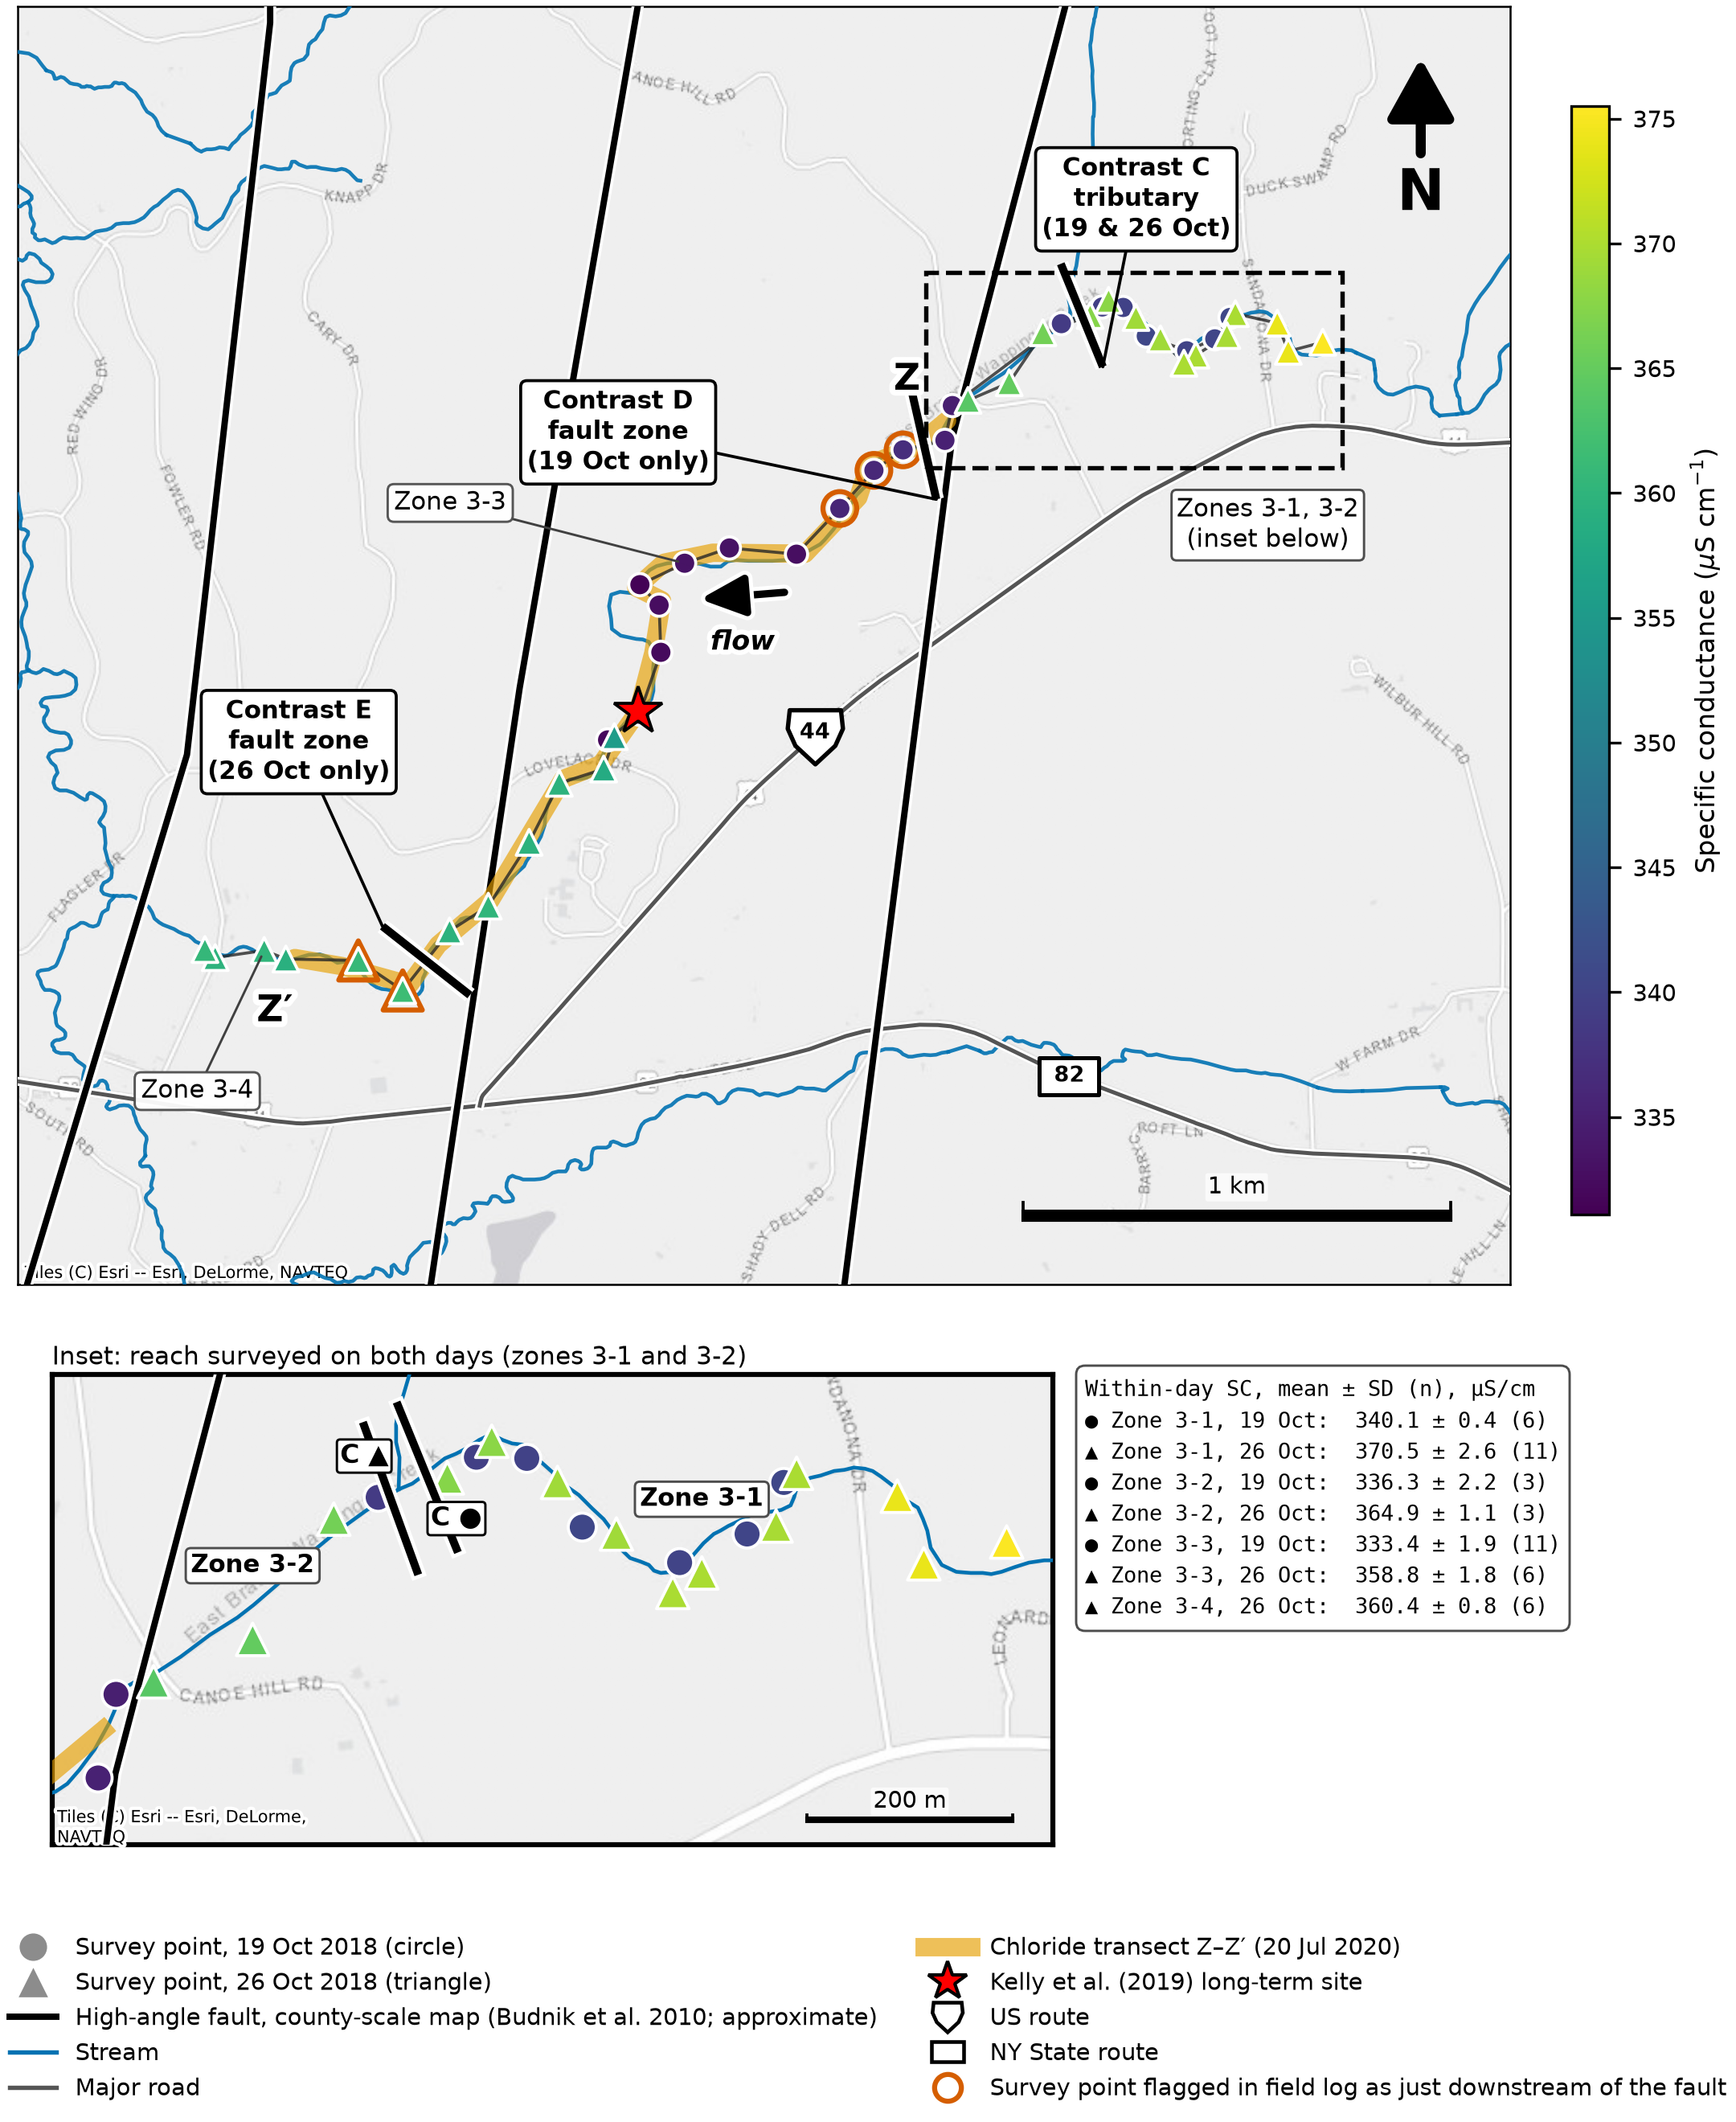
\includegraphics[width=0.85\linewidth]{figures/rev_site3.png}
	\caption{\DIFaddFL{Site 3 and Contrasts C, D and E. Circles are 19 October and triangles 26 October 2018 points; the two days differ by about 28~$\mu$S/cm, so zones are compared within a day only. The inset enlarges the reach surveyed on both days. The yellow band is the 2020 chloride transect (Z--Z$'$) and the red star the monitoring site of \mbox{%DIFAUXCMD
\citet{kelly2019}}\hskip0pt%DIFAUXCMD
.}}
	\label{fig:site3}
\end{figure}

\textbf{\DIFadd{Pooling days.}} \linelabel{L:pooling}\DIFadd{When the two survey days are pooled, Contrast E appears as a rise of $+18.0$~$\mu$S/cm ($p < 0.001$), larger than any other step in the survey. That value is an artefact of pooling two survey days. Zone 3-3 would then combine 11 points from 19 October (333.4~$\mu$S/cm) with 6 from 26 October (358.8~$\mu$S/cm), giving a pooled mean of 342.4~$\mu$S/cm, whereas Zone 3-4 consists only of 26 October points. The ``step'' is the difference between days, not a change along the channel; }\linelabel{L:pooling-sd}\DIFadd{the same pooling inflates the zone standard deviations to 12.6--15.8~$\mu$S/cm, against 0.4--2.6~$\mu$S/cm within a day.
}

\textbf{\DIFadd{Day offset and the repeated reach.}} \DIFadd{Eleven 19 October points have a 26 October point within 120~m, and the pairs differ by 23.5--29.7~$\mu$S/cm (mean 27.8, SD 2.2); }\linelabel{L:offset-seam}\DIFadd{two points 18~m apart at the seam between the surveys read 332.0 }\DIFaddend and \DIFdelbegin \DIFdel{the second fault crossing (Contrast E)produces the largest step of the entire study, an 18.0}\DIFdelend \DIFaddbegin \DIFadd{355.5}\DIFaddend ~$\mu$S/cm\DIFdelbegin \DIFdel{rise significant at $p < 0.001$. The spatial coincidence of the strongest increase with a mapped fault}\DIFdelend \DIFaddbegin \DIFadd{. The offset is therefore not constant}\DIFaddend , and its \DIFdelbegin \DIFdel{absence at the tributary, is the core observation the statistics support. }\DIFdelend \DIFaddbegin \DIFadd{range of about 6~$\mu$S/cm exceeds Contrasts B and E, which is why we neither pooled days nor corrected for it. }\linelabel{L:offset-repeat}\DIFadd{Zones 3-1 and 3-2 were surveyed on both days (Figure~\ref{fig:site3}, inset): Zone 3-1 averaged 340.1 $\pm$ 0.4~$\mu$S/cm ($n = 6$) on 19 October and 370.5 $\pm$ 2.6 ($n = 11$) on 26 October, and Zone 3-2 averaged 336.3 $\pm$ 2.2 ($n = 3$) and 364.9 $\pm$ 1.1 ($n = 3$), so within each day the zones are internally consistent but the two days differ by about 29--30~$\mu$S/cm.
}\DIFaddend 

\DIFdelbegin %DIFDELCMD < \begin{figure}[htbp]
%DIFDELCMD < 	\centering
%DIFDELCMD < 	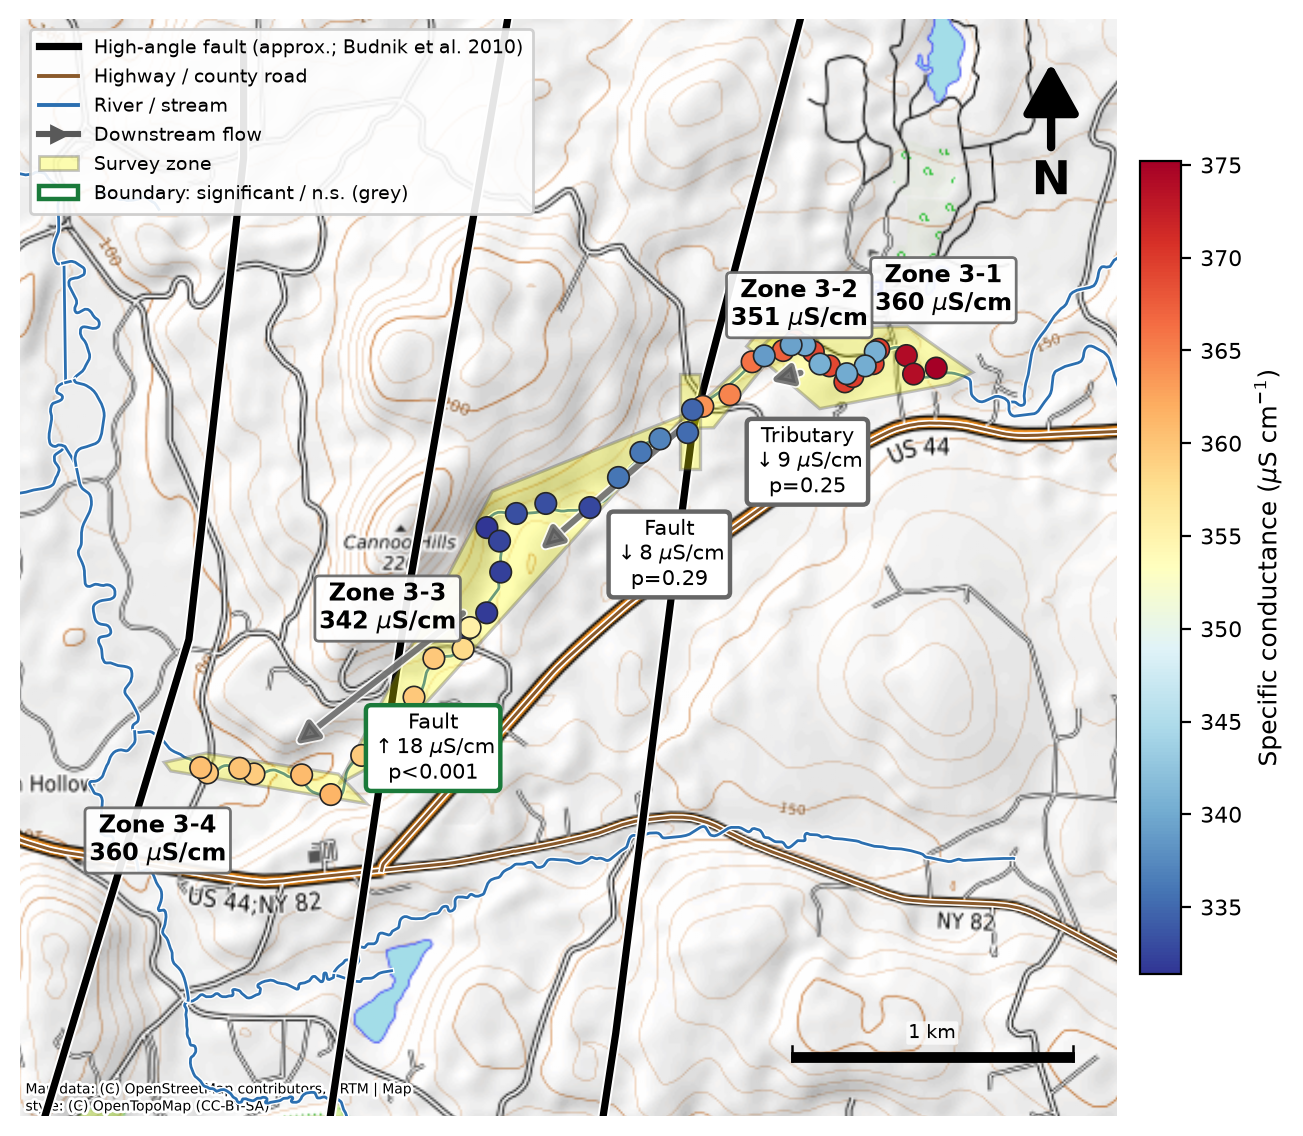
\includegraphics[width=0.85\linewidth]{figures/site3.png}
%DIFDELCMD < 	%%%
%DIFDELCMD < \caption{%
{%DIFAUXCMD
\DIFdelFL{Site 3, symbolised as in Figure~\ref{fig:site1}: terrain base, roads (brown) and streams (blue), survey points coloured by specific conductance, and red-outlined survey zones labelled with their mean specific conductance. Zones are numbered in ascending order downstream. High-angle faults (thick black) are approximate, digitized from \mbox{%DIFAUXCMD
\citet{budnik2010}}\hskip0pt%DIFAUXCMD
. Across the fault crossing between Zones 3-3 and 3-4 the mean specific conductance increases sharply, whereas the tributary junction and the weaker fault crossing show little change; statistical comparisons are given in Table~\ref{tab:ttest}.}}
	%DIFAUXCMD
%DIFDELCMD < \label{fig:site3}
%DIFDELCMD < \end{figure}
%DIFDELCMD < %%%
\DIFdelend \DIFaddbegin \subsection{\DIFadd{Chloride transect}}
\DIFaddend 

\DIFdelbegin \DIFdel{Chloride sampling showed chloride measurements consistent with the long-term studies shown by Kelly et al.
2019 \mbox{%DIFAUXCMD
\citep{kelly2019} }\hskip0pt%DIFAUXCMD
}\DIFdelend \DIFaddbegin \linelabel{L:cl-start}\DIFadd{The 20 July 2020 transect }\DIFaddend (Figure~\ref{fig:chloride}) \DIFdelbegin \DIFdel{. Strong contrasts in chloride occurred close to where the geological fault line exists with concentration peaking $\sim$1000 meters upstream of }\DIFdelend \DIFaddbegin \DIFadd{ran 2}{\DIFadd{,}}\DIFadd{351~m from Z to Z$'$, starting near the survey points flagged for Contrast D and ending just downstream of those flagged for Contrast E, so it lies mostly within Zone 3-3. }\linelabel{L:cl-peaks}\DIFadd{Chloride across the 18 main-stem samples ranged from 13.75 to 50.0~mg/L, with }\DIFaddend the \DIFdelbegin \DIFdel{long-term study point. Because this transect was collected in summer, nearly two years after the conductivity survey, its agreement with the Contrast E crossing corroborates the specific-conductance step with an independent ion, in an independent year, and under baseflow conditions when direct road-salt runoff is not occurring. The chloride peak thus reinforces the interpretation that groundwater discharging near the fault, rather than surface runoff, carries the elevated salt into this reach. }\DIFdelend \DIFaddbegin \DIFadd{highest values at 474~m (50.0~mg/L), 690~m (36.25~mg/L) and 959~m (40.0~mg/L). These lie 133--468~m from the nearest flagged point for Contrast D and 293--391~m from the nearest digitized fault trace. }\linelabel{L:cl-bp}\DIFadd{The segmented regression selects one breakpoint at 467~m (bootstrap interval 308--800~m), where the fitted slope changes from $+53$ to $-15$~mg/L per km; the change-in-mean analysis places shifts at 384 and 1021~m. The breakpoint is about 125~m from the nearest Contrast D flagged point and about 300~m from the nearest trace, but it is driven largely by the single 50~mg/L sample. }\linelabel{L:cl-E}\DIFadd{Near Contrast E, chloride is low and flat: only 2 of the 18 samples lie downstream of the Contrast E flagged points (13.75 and 15.0~mg/L), and the last five samples are 13.75--17.5~mg/L. The transect therefore shows no chloride increase at Contrast E. With so few points downstream of E we did not attempt a two-sample test.
}\DIFaddend 

\begin{figure}[htbp]
	\centering
	\DIFdelbeginFL %DIFDELCMD < 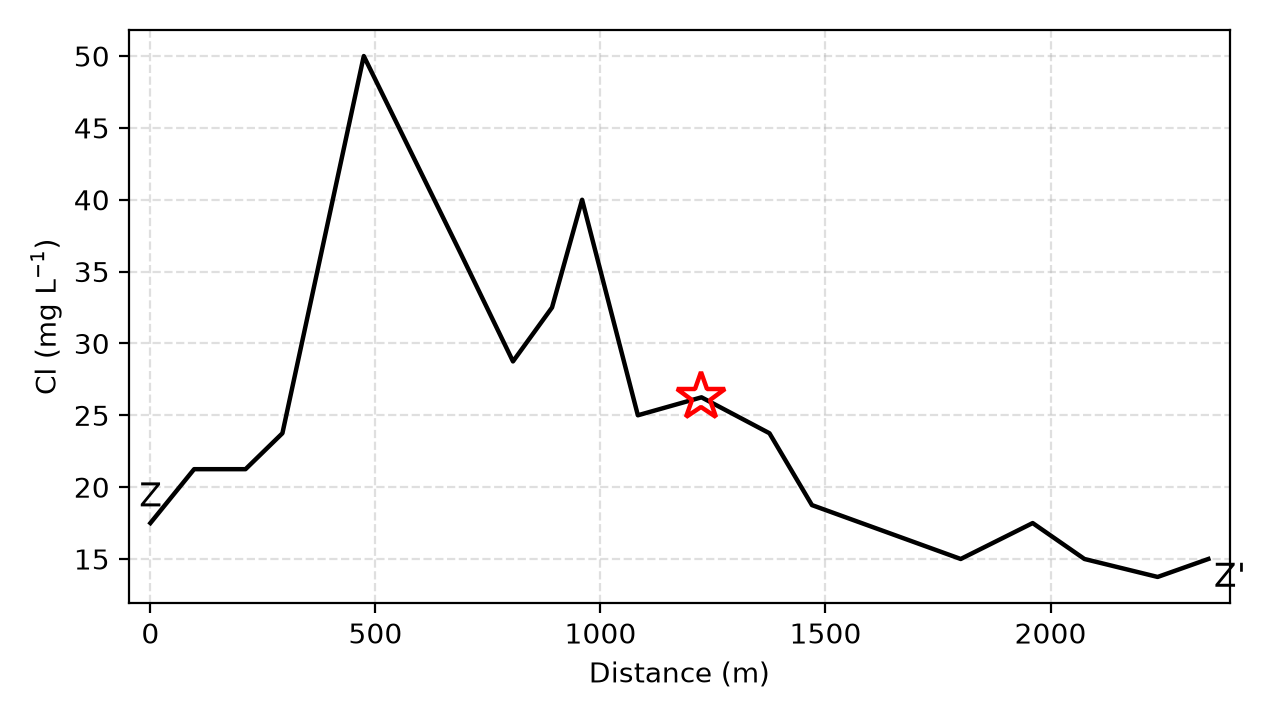
\includegraphics[width=0.71\linewidth]{figures/chloride.png}
%DIFDELCMD < 	%%%
\DIFdelendFL \DIFaddbeginFL 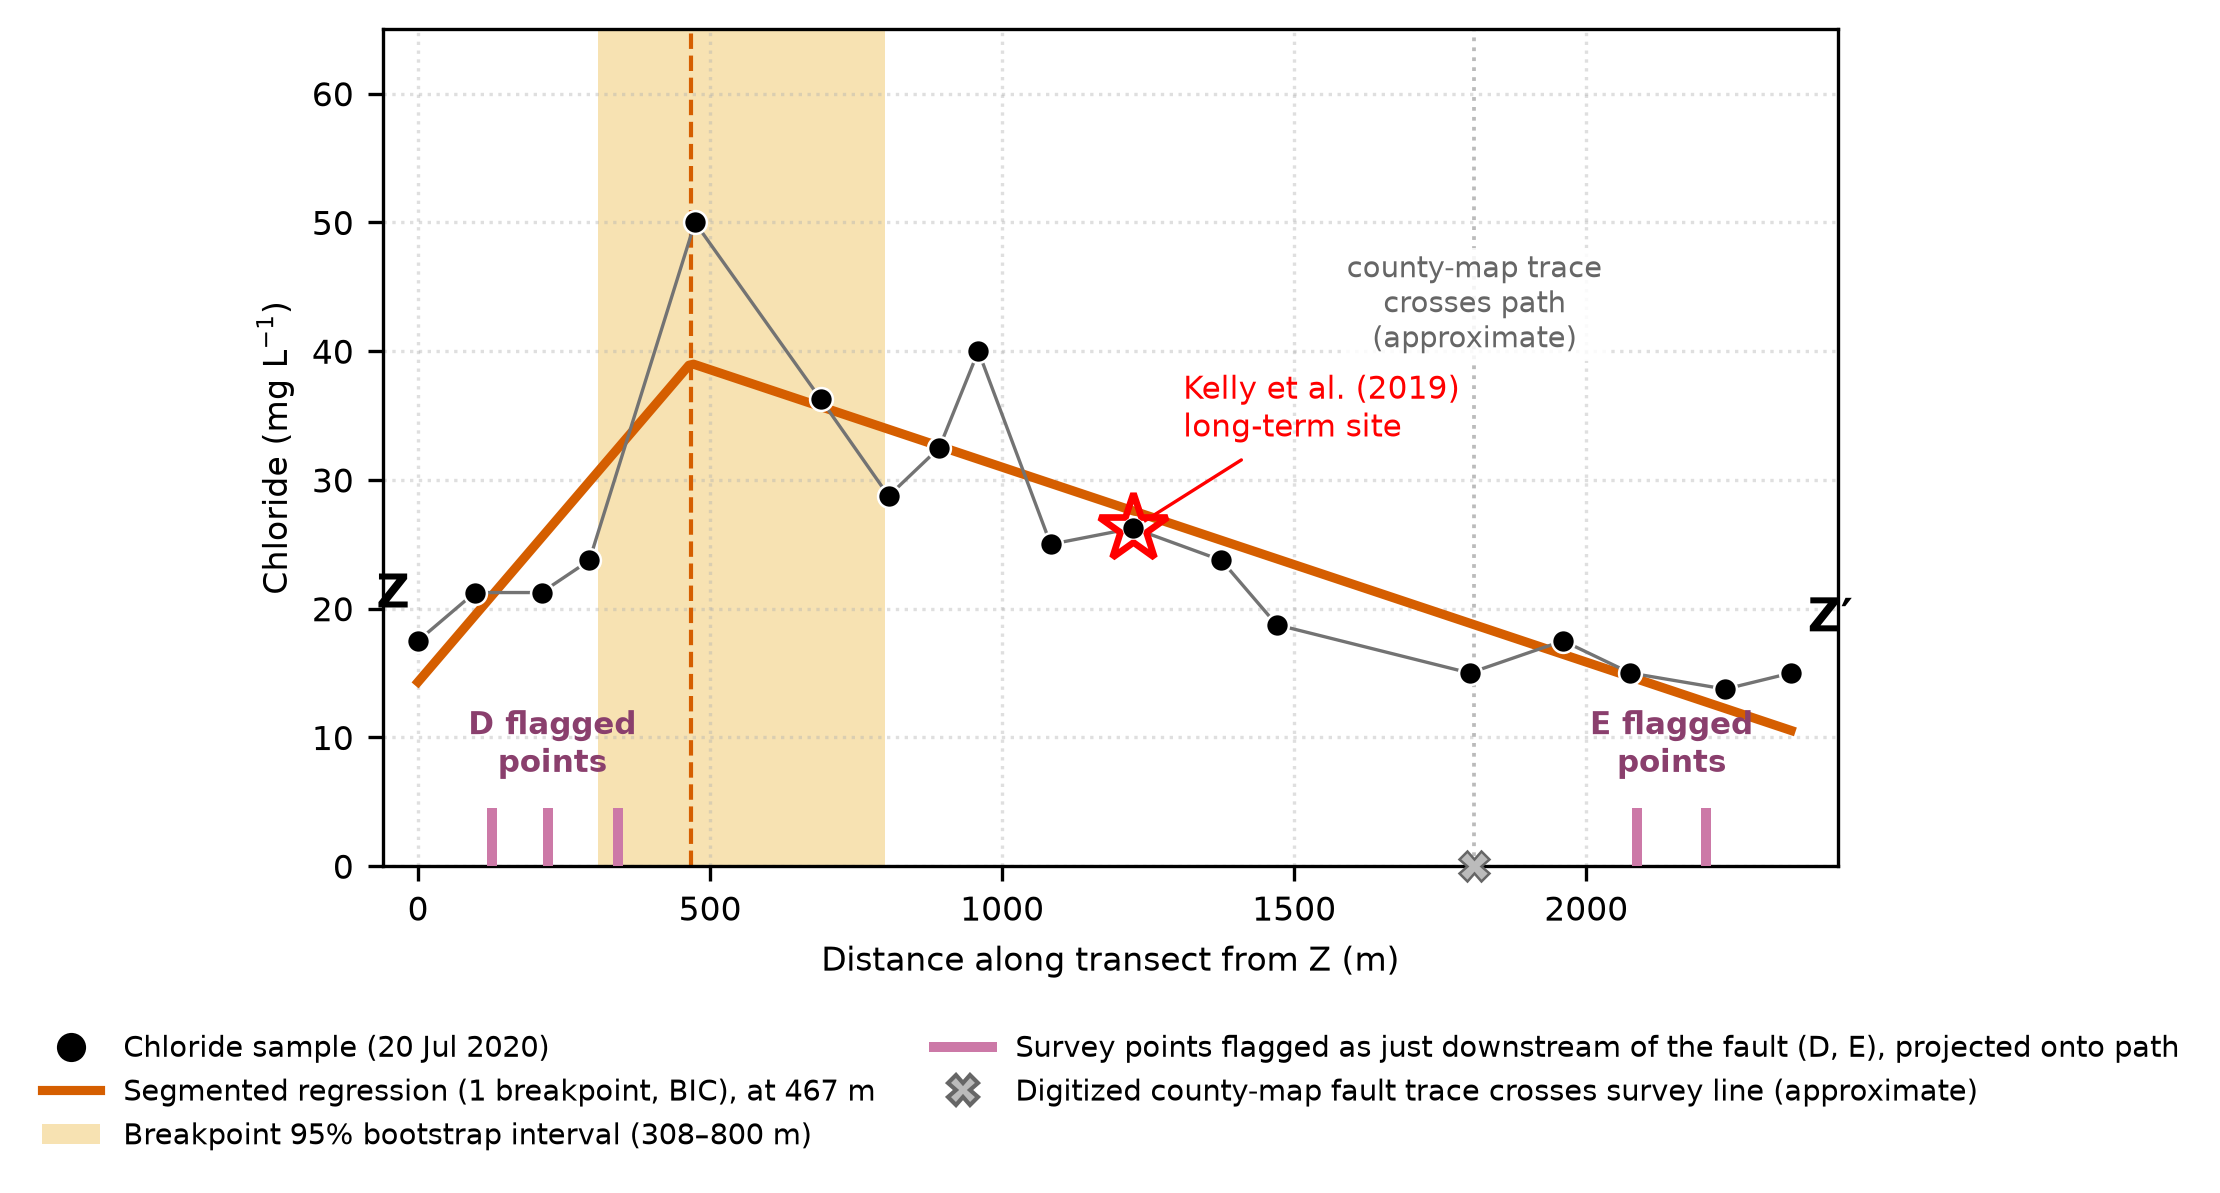
\includegraphics[width=0.9\linewidth]{figures/rev_chloride.png}
	\DIFaddendFL \caption{Chloride \DIFdelbeginFL \DIFdelFL{measurements }\DIFdelendFL along \DIFdelbeginFL \DIFdelFL{zones 3-3 and 3-4 shown in relative distance from points Z to Z'}\DIFdelendFL \DIFaddbeginFL \DIFaddFL{the 20 July 2020 transect (Z--Z$'$)}\DIFaddendFL . The \DIFaddbeginFL \DIFaddFL{orange line is the segmented fit, with its breakpoint (467~m) and 95\% interval (tan); the breakpoint rests largely on the single 50~mg/L sample. Pink ticks mark points logged as just downstream of the faults at Contrasts D and E, the blue cross the mapped fault crossing, and the }\DIFaddendFL red star \DIFdelbeginFL \DIFdelFL{indicates }\DIFdelendFL the \DIFdelbeginFL \DIFdelFL{sampling point from the 32-year dataset introduced by Kelly et al}\DIFdelendFL \DIFaddbeginFL \DIFaddFL{monitoring site of \mbox{%DIFAUXCMD
\citet{kelly2019}}\hskip0pt%DIFAUXCMD
}\DIFaddendFL .\DIFdelbeginFL \DIFdelFL{2019 \mbox{%DIFAUXCMD
\citep{kelly2019}}\hskip0pt%DIFAUXCMD
.}\DIFdelendFL }
	\label{fig:chloride}
\end{figure}

\subsection{\DIFdelbegin \DIFdel{Two-sample $t$-test}\DIFdelend \DIFaddbegin \DIFadd{Change-point analysis of specific conductance}\DIFaddend }

\DIFdelbegin \DIFdel{Each contrast compares two adjacent reaches of Wappinger Creek separated by a geologic feature, tested with a two-sample Welch $t$-test on the raw }\DIFdelend \DIFaddbegin \linelabel{L:cp-none}\DIFadd{Segmented regression and a change-in-mean check on each single-day transect (Figure~\ref{fig:changepoint}) find no }\DIFaddend specific-conductance \DIFdelbegin \DIFdel{measurements (Table~\ref{tab:ttest}) . Here $\bar{x}_1$ and $\bar{x}_2$ are the upstream and downstream zone means (}\DIFdelend \DIFaddbegin \DIFadd{breakpoint at a fault contrast boundary or at a point where the digitized trace crosses the transect. }\linelabel{L:cp-site2}\DIFadd{At Site 2 one breakpoint is selected at 2}{\DIFadd{,}}\DIFadd{355~m (bootstrap interval 1}{\DIFadd{,}}\DIFadd{327--3}{\DIFadd{,}}\DIFadd{384~m), after which conductance rises steadily downstream; the fitted slope increases from 0.1 to 1.6~}\DIFaddend $\mu$S/cm \DIFdelbegin \DIFdel{), $n_1$ and $n_2$ their sample sizes,and the ``Boundary'' column records whether the separating feature is a mapped fault crossing or a tributary junction. At a significance threshold of $\alpha = 0.05$, }\DIFdelend \DIFaddbegin \DIFadd{per km. This breakpoint lies about 1.6~km upstream of the Contrast B boundary, }\DIFaddend the \DIFdelbegin \DIFdel{two fault crossings with the clearest geometry (Contrasts B and E) show significant increases in specific conductance ($p < 0.001$) ; the third fault crossing (Contrast D) and the two tributary-confounded contrasts (A and C) do not reach significance. A nonparametric Mann--Whitney $U$ test gives the same picture for B, D, }\DIFdelend \DIFaddbegin \DIFadd{field-interpreted fault position at the channel bend (3}{\DIFadd{,}}\DIFadd{993~m; 0.6--2.7~km given the bootstrap interval); the change-in-mean analysis places three small shifts ($+1.5$, $+2.3$ }\DIFaddend and \DIFdelbegin \DIFdel{E}\DIFdelend \DIFaddbegin \DIFadd{$+3.3$~$\mu$S/cm) between 2.6 and 5.9~km. }\linelabel{L:cp-contrastB}\DIFadd{Contrast B is therefore better described as part of a gradual downstream ramp than as an abrupt step at the interpreted fault position. At Site 1 and on the 19 October Site 3 transect no breakpoint is selected (for 19 October a one-breakpoint model ties with none, $\Delta$BIC = 0.03). On the upper 26 October Site 3 transect two breakpoints (300 and 459~m) are only marginally preferred ($\Delta$BIC = 0.3) and lie 314--473~m from the tributary and away from any trace. On the lower 26 October transect (Contrast E) one breakpoint is selected at 194~m, where conductance rises from 355.5 to 359.7~$\mu$S/cm over the first 190~m and then stays near 360~$\mu$S/cm. }\linelabel{L:cp-E-min}\DIFadd{This breakpoint sits at the minimum segment length the method allows, 330~m upstream of where the channel crosses the digitized trace (at 523~m), 123~m in straight-line distance from the nearest trace, and 522~m upstream of the Contrast E boundary}\DIFaddend .

%DIF <  Table auto-generated by src/stats.py from data/salinity-dataset.xlsx.
\DIFaddbegin \begin{figure}[htbp]
	\centering
	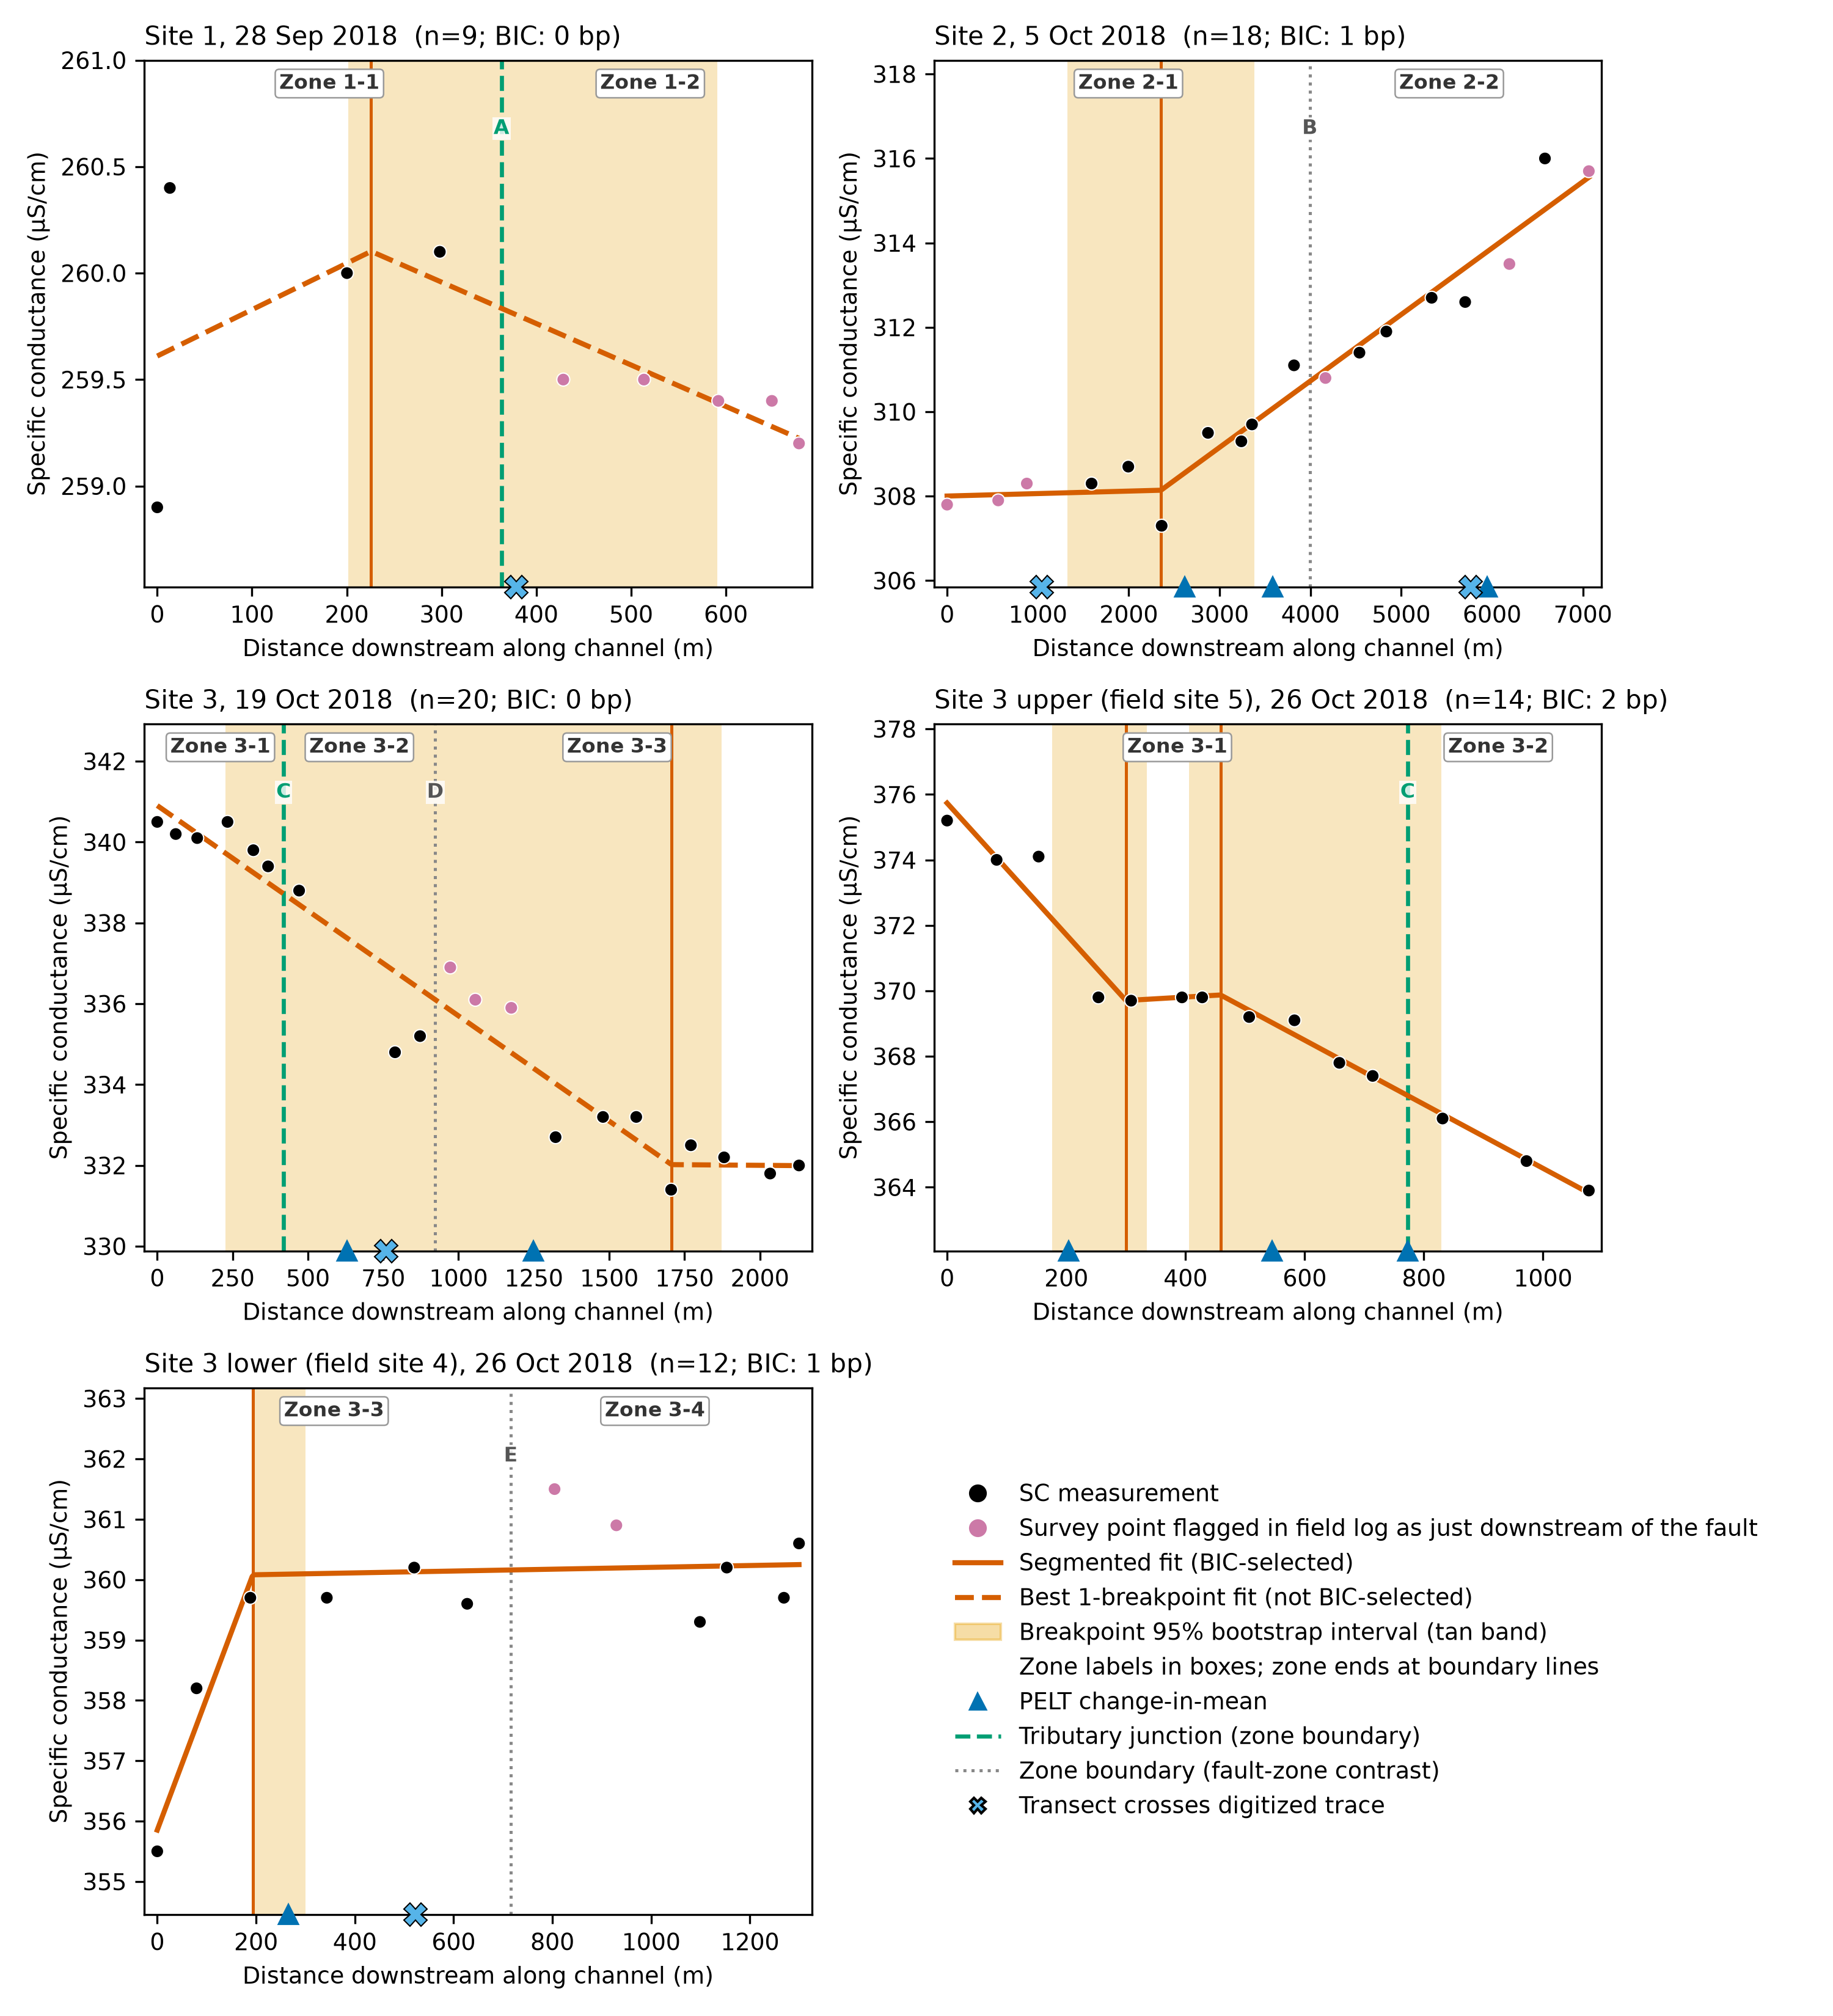
\includegraphics[width=\linewidth]{figures/rev_changepoint_sc.png}
	\caption{\DIFaddFL{Specific conductance along each single-day transect, with segmented fits (orange; dashed where no breakpoint is selected) and 95\% breakpoint intervals (tan). Pink points were logged as just downstream of a fault; blue triangles are change-in-mean shifts; blue crosses are mapped fault crossings; green and grey lines are tributary and fault-contrast zone boundaries.}}
	\label{fig:changepoint}
\end{figure}

%DIF >  Tables 1 and 2 are placed here, after the Results text that cites them.
\DIFaddend \begin{table}[htbp]
	\caption{\DIFdelbeginFL \DIFdelFL{Two-sample Welch $t$-test results for each upstream}\DIFdelendFL \DIFaddbeginFL \DIFaddFL{Within-day zone contrasts in specific conductance ($\mu$S}\DIFaddendFL /\DIFdelbeginFL \DIFdelFL{downstream contrast}\DIFdelendFL \DIFaddbeginFL \DIFaddFL{cm)}\DIFaddendFL . \DIFdelbeginFL \DIFdelFL{Contrasts B }\DIFdelendFL \DIFaddbeginFL \DIFaddFL{$\Delta$ is downstream minus upstream, with its Welch 95\% CI; $U$ }\DIFaddendFL and \DIFdelbeginFL \DIFdelFL{E (fault crossings) }\DIFdelendFL \DIFaddbeginFL \DIFaddFL{$p_{\mathrm{MW}}$ }\DIFaddendFL are \DIFdelbeginFL \DIFdelFL{significant at $\alpha = 0.05$}\DIFdelendFL \DIFaddbeginFL \DIFaddFL{from the Mann--Whitney test}\DIFaddendFL . \DIFaddbeginFL \DIFaddFL{$^\dagger$ marks a zone with fewer than five points.}\DIFaddendFL }
	\centering
	\DIFdelbeginFL %DIFDELCMD < % Auto-generated by src/stats.py -- do not edit by hand.
\begin{tabular}{cclccrrrc}
\toprule
Contrast & Zones & Boundary & $n_1$ & $n_2$ & $\bar{x}_1$ & $\bar{x}_2$ & Welch $t$ & $p$ \\
\midrule
A & 1-1, 1-2 & tributary & 4 & 5 & 259.9 & 259.4 & -1.35 & 0.264 \\
B & 2-1, 2-2 & fault & 10 & 8 & 308.8 & 313.1 & 5.63 & $<$0.001 \\
C & 3-1, 3-2 & tributary & 17 & 6 & 359.8 & 350.6 & -1.24 & 0.248 \\
D & 3-2, 3-3 & fault & 6 & 17 & 350.6 & 342.4 & -1.15 & 0.286 \\
E & 3-3, 3-4 & fault & 17 & 6 & 342.4 & 360.4 & 5.83 & $<$0.001 \\
\bottomrule
\end{tabular}

%DIFDELCMD < 	%%%
\DIFdelendFL \DIFaddbeginFL \scriptsize
	\setlength{\tabcolsep}{3pt}
	\resizebox{\linewidth}{!}{% Auto-generated by src/within_day.py -- do not edit by hand.
% Within-single-day contrasts. Delta = downstream - upstream (uS/cm). n<=3 in a zone: interpret with great caution.
\begin{tabular}{llllrrrrrrrr}
\toprule
Contr. & Boundary & Date & Zones & $n_1,n_2$ & Up (mean$\pm$SD) & Down (mean$\pm$SD) & $\Delta$ [95\% CI] & Welch $t$ (df) & $p$ & $U$ & $p_{\mathrm{MW}}$ \\
\midrule
A & tributary & 28 Sep & 1-1$\rightarrow$1-2 & 4,5$^{\dagger}$ & 259.9$\pm$0.7 & 259.4$\pm$0.1 & -0.5 [-1.5, +0.6] & -1.35 (3.2) & 0.264 & 5 & 0.266 \\
B & fault & 5 Oct & 2-1$\rightarrow$2-2 & 10,8 & 308.8$\pm$1.1 & 313.1$\pm$1.9 & +4.3 [+2.6, +6.0] & 5.63 (10.8) & $<$0.001 & 79 & $<$0.001 \\
C & tributary & 19 Oct & 3-1$\rightarrow$3-2 & 6,3$^{\dagger}$ & 340.1$\pm$0.4 & 336.3$\pm$2.2 & -3.8 [-9.2, +1.5] & -2.97 (2.1) & 0.093 & 0 & 0.028 \\
C & tributary & 26 Oct & 3-1$\rightarrow$3-2 & 11,3$^{\dagger}$ & 370.5$\pm$2.6 & 364.9$\pm$1.1 & -5.6 [-7.9, -3.3] & -5.48 (8.8) & $<$0.001 & 0 & 0.012 \\
D & fault & 19 Oct & 3-2$\rightarrow$3-3 & 3,11$^{\dagger}$ & 336.3$\pm$2.2 & 333.4$\pm$1.9 & -2.8 [-7.4, +1.7] & -2.02 (2.9) & 0.140 & 6 & 0.119 \\
E & fault & 26 Oct & 3-3$\rightarrow$3-4 & 6,6 & 358.8$\pm$1.8 & 360.4$\pm$0.8 & +1.6 [-0.3, +3.4] & 1.96 (7.0) & 0.090 & 30 & 0.076 \\
\bottomrule
\end{tabular}
% $^{\dagger}$ one zone has fewer than 5 points (add to the caption).
}
	\DIFaddendFL \label{tab:ttest}
\end{table}

\DIFaddbegin \begin{table}[htbp]
	\caption{\DIFaddFL{Autocorrelation-adjusted tests and road distances for Table~\ref{tab:ttest}. $\hat\rho_1$ is the lag-1 autocorrelation and $n_{\mathrm{eff}} = n(1-\rho)/(1+\rho)$ the effective sample size; adjusted $p$-values are a sensitivity check. Road distances are zone medians to the nearest primary or secondary road (excluding the Taconic State Parkway) and were not tested.}}
	\centering
	\small
	% Auto-generated by src/within_day.py -- do not edit by hand.
\begin{tabular}{lllrrrrrrr}
\toprule
Contr. & Date & Zones & $\hat\rho_1$ & $n_{\mathrm{eff},1}$ & $n_{\mathrm{eff},2}$ & $p$ (Welch) & $p$ ($n_{\mathrm{eff}}$) & \multicolumn{2}{c}{Median road dist. (m)} \\
\cmidrule(lr){9-10}
 & & & & & & & & up & down \\
\midrule
A & 28 Sep & 1-1$\rightarrow$1-2 & -0.27 & 4.0 & 5.0 & 0.264 & 0.264 & 927 & 751 \\
B & 5 Oct & 2-1$\rightarrow$2-2 & 0.37 & 4.6 & 3.7 & $<$0.001 & 0.017 & 335 & 726 \\
C & 19 Oct & 3-1$\rightarrow$3-2 & -0.35 & 6.0 & 3.0 & 0.093 & 0.093 & 304 & 425 \\
C & 26 Oct & 3-1$\rightarrow$3-2 & 0.54 & 3.2 & 2.0 & $<$0.001 & 0.041 & 245 & 414 \\
D & 19 Oct & 3-2$\rightarrow$3-3 & 0.35 & 2.0 & 5.3 & 0.140 & 0.279 & 425 & 409 \\
E & 26 Oct & 3-3$\rightarrow$3-4 & 0.30 & 3.2 & 3.2 & 0.090 & 0.243 & 312 & 368 \\
\bottomrule
\end{tabular}

	\label{tab:support}
\end{table}

\DIFaddend \section{Discussion}

\subsection{\DIFdelbegin \DIFdel{Contrasts}\DIFdelend \DIFaddbegin \DIFadd{What the survey shows}\DIFaddend }

\DIFdelbegin \DIFdel{Two contrasts showed statistically significant changes in specific conductance: Contrasts B and E, from Sites 2 and 3 respectively. Each is a fault crossing, and each showed a statistically significant increase in specific conductance after the fault line interaction at $\alpha$ = 0.05, indicating a likely increase in stream salinity. The tributary-confounded contrasts A and C both showed decreases in specific conductance that did not reach significance; in any case these do not bear on our main conclusion about faults, because each corresponded to the location of an active tributary inputting water to the main stem of the creek, and measurements at Site 1 were taken during a rain event that occurred during sampling that day. The salinity levels for this section of the creek were between 50--100}\DIFdelend \DIFaddbegin \linelabel{L:disc-answer}\DIFadd{The question posed by the title is whether fault zones route road-salt-contaminated groundwater to streams. The survey does not answer it clearly. Of the three contrasts at mapped faults, one shows a small, significant increase in specific conductance (Contrast B, $+4.3$}\DIFaddend ~$\mu$S/\DIFaddbegin \DIFadd{cm), one shows a non-significant decrease (Contrast D, $-2.8$~$\mu$S/}\DIFaddend cm\DIFdelbegin \DIFdel{lower than the measurements taken at the other two sites. At Contrast C the active tributary measured nearly 150}\DIFdelend \DIFaddbegin \DIFadd{) and one shows a non-significant increase within instrument accuracy (Contrast E, $+1.6$}\DIFaddend ~$\mu$S/cm\DIFdelbegin \DIFdel{lower than the specific conductance measurements at Zones 3-1 and 3-2}\DIFdelend \DIFaddbegin \DIFadd{). No conductance breakpoint on any transect coincides with a fault contrast boundary}\DIFaddend .

\DIFdelbegin \DIFdel{Of the three fault crossings that do not coincide with an active tributary (Contrasts B, D, and E), two showed a statistically significant increase in specific conductance, while the third, }\DIFdelend \DIFaddbegin \DIFadd{Contrast B is an observation worth testing, not evidence of fault transport. It is a gradual rise that begins roughly 1.6~km upstream of the zone boundary, which marks the fault position we interpreted in the field at an abrupt channel bend, along a reach where the county-scale fault trace runs parallel to the creek and cannot show where the fault meets the channel. A rise of this kind is what diffuse groundwater input, or a fault-parallel flowpath delivering water along the reach, would both produce, and the survey cannot tell them apart. }\linelabel{L:disc-D}\DIFaddend Contrast D, \DIFdelbegin \DIFdel{did not reach significance at $\alpha$ = 0.05 (Welch $t$ = $-1.15$, $p$ = 0.286). We do not read the non-significant crossing as evidence against fault-mediated transport. Contrast D compares the two zones with the most unequal sample sizes ($n_1$ = 6}\DIFdelend \DIFaddbegin \DIFadd{at a fault with no tributary, shows no increase. }\linelabel{L:disc-E}\DIFadd{Contrast E is within the instrument's stated accuracy and its only breakpoint lies near the start of a short transect, 330~m upstream of where the channel crosses the trace. The 2020 chloride transect adds a further observation worth testing: its peak lies near the Contrast D flagged points and about 300~m from the nearest trace}\DIFaddend , \DIFdelbegin \DIFdel{$n_2$ = 17; Table~\ref{tab:ttest}) and lies immediately downstream of the tributary-diluted Zone 3-2, so its two reaches begin from different baseline concentrations and the comparison carries the least statistical power of the five. A single non-significant crossing bounds the strength of any inference we can draw from three examples, }\DIFdelend but it \DIFdelbegin \DIFdel{does not weaken the significant increases at Contrasts B and E, each of which recovered a clear signal from the same small-sample setting. We therefore present these three crossings as an initial, spatially explicit example of the pattern rather than as a population-level test of it. Later additional observation of longitudinal chloride concentrations across Contrast E (Figure~\ref{fig:chloride}, Z to Z')indicated the same strong contrastassociated spatially with mapped fault locations}\DIFdelend \DIFaddbegin \DIFadd{rests on one sample, comes from a different year, and chloride near Contrast E is low (about 14--15~mg/L)}\DIFaddend . \DIFaddbegin \linelabel{L:disc-clpeak}\DIFadd{We do not treat the chloride peak as support for the conductance result at any contrast.
}\DIFaddend 

\DIFdelbegin \DIFdel{A published 32-year dataset \mbox{%DIFAUXCMD
\citep{kelly2019} }\hskip0pt%DIFAUXCMD
from the same stream reach as our study (Figure~\ref{fig:site3}, star; Figure~\ref{fig:chloride}, Z to Z') indicated that stream chloride has gradually increased in the area from annual means of roughly 15~mg/l in the 1980s to over 40~mg/l for annual means by }\DIFdelend \DIFaddbegin \DIFadd{The tributary contrast is an internal check. Contrast C decreases conductance on both days, as two-end-member mixing predicts when lower-conductance water joins the main stem \mbox{%DIFAUXCMD
\citep{genereux1998}}\hskip0pt%DIFAUXCMD
, so the survey can detect a known input of }\DIFaddend the \DIFdelbegin \DIFdel{2010s. This increase through time, as well as other findings \mbox{%DIFAUXCMD
\citep{kelly2019}}\hskip0pt%DIFAUXCMD
, suggest a strong tie to human applications of road salt in the region. The elevated levels in streamflow in summer strongly suggest artificially elevated chloride levels overall, well above geologic background levels in groundwater. However, this study used only one location of data collection for long-term work on the stream \mbox{%DIFAUXCMD
\citep{kelly2019}}\hskip0pt%DIFAUXCMD
, and was therefore not able to look at the spatial aspect of possible fault controls as transport pathways for road salts, as we have here. This new spatial conductivity and chloride data (Figure~\ref{fig:chloride}), in combination with the findings of similar concentrations of chloride during this extensive long-term study in the same stream stretch \mbox{%DIFAUXCMD
\citep{kelly2019}}\hskip0pt%DIFAUXCMD
, together offer a much stronger link to road salts and their spatial controls on transport from faults. Collectively, this provides strong initial evidence that linear fault zones are indeed aiding in the preferential input of salt-polluted groundwater into streams at locations that correspond to where these major km-scale geologic structures connect both streams and highways}\DIFdelend \DIFaddbegin \DIFadd{size we are discussing. }\linelabel{L:disc-mask}\DIFadd{Dilution by a tributary could in principle also mask a groundwater input entering at the same place, which would hide a fault signal at Contrast C; we cannot test that possibility without discharge measurements.
}

\DIFadd{The size of the differences also matters. The stated accuracy of the conductivity measurement is a bound on absolute error, and a calibration offset common to all readings on one day cancels in a within-day difference, but random reading error does not, and the manufacturer gives no repeatability figure. }\linelabel{L:disc-size}\DIFadd{Contrast B exceeds that bound by a factor of about 2.5 and exceeds the within-zone scatter, which is why we report it as a real but small difference; Contrast E does not exceed it. Site 1, where a coincident tributary and very high flow after rain confound the only contrast, contributes little either way. }\linelabel{L:disc-screening}\DIFadd{Taken together, the survey is best read as a screening result: it shows what a low-cost survey can detect, namely a small gradual rise at one site and the dilution at a tributary, and it also shows that such a survey does not locate a fault-related input to within the spacing of a few hundred metres that a fault trace of uncertain position would require}\DIFaddend .

\subsection{\DIFdelbegin \DIFdel{Addressing possible alternative sources of salinity in Wappinger Creek}\DIFdelend \DIFaddbegin \DIFadd{Alternative explanations}\DIFaddend }

\DIFdelbegin \DIFdel{Increases in salinity can also occur as salts naturally enter the environment through the geological weathering of rock surfaces \mbox{%DIFAUXCMD
\citep{nimiroski2002}}\hskip0pt%DIFAUXCMD
.
The bedrock below Wappinger Creek consists of metamorphosed clastic sedimentary rocks \mbox{%DIFAUXCMD
\citep{budnik2010} }\hskip0pt%DIFAUXCMD
known to have minimal influence of stream salt input. A 2008 study of sodium chloride retention in the east branch of Wappinger Creek (a portion of our study site)identified average salt input to the stream from various sources such as road salt, parking area salt, sewage, or rock weathering. The result found road salt contributes to 83\% of stream salt input, while geological rock weathering accounts for only 1\% of the input \mbox{%DIFAUXCMD
\citep{kelly2008}}\hskip0pt%DIFAUXCMD
. Therefore, we argue that rock weathering is likely a tiny portion of total stream salt input and cannot account for the inferred changes in salinity we observed along fault zones in our study. This local partitioning is consistent with }\DIFdelend \DIFaddbegin \linelabel{L:alt-start}\DIFadd{Several explanations for the Site 2 increase, and for the conductance differences generally, are at least as plausible as fault-routed groundwater with the data in hand.
}

\emph{\DIFadd{Road proximity.}} \DIFadd{Per-zone median distances from survey points to }\DIFaddend the \DIFdelbegin \DIFdel{wider regional picture. Syntheses of the anthropogenic salt cycle attribute the accelerating mobilization and accumulation of salt in temperate watersheds to human activities, with road deicing prominent among them \mbox{%DIFAUXCMD
\citep{kaushal2023saltcycle}}\hskip0pt%DIFAUXCMD
, and mass-balance work across a comparable metropolitan region shows that a large fraction of applied road salt is retained in , and only slowly released from, groundwaterrather than flushed directly to streams \mbox{%DIFAUXCMD
\citep{vanmeter2024}}\hskip0pt%DIFAUXCMD
. Both lines of evidence point to a mobile, human-derived chloride pool held in the subsurface, precisely the pool that a conductive fault could route preferentially toward the channel. The elevated summer conductivities we recorded, at a time of year when direct road-salt runoff is absent, are difficult to reconcile with a purely geologic source and instead implicate this stored anthropogenic salt.
Stream salinity can also rise }\DIFdelend \DIFaddbegin \DIFadd{nearest major road range from 245 to 927~m (Table~\ref{tab:support}). }\linelabel{L:alt-road-site2}\DIFadd{At Site 2 the downstream zone is farther from a major road than the upstream zone (median 726 versus 335~m), so proximity to a major road does not by itself explain Contrast B, although one upstream point lies only 39~m from a road and the distances do not capture drainage or road density. The Site 3 zones lie 245--425~m from the nearest major road, mainly US 44, with no monotone relation to the conductance pattern. }\linelabel{L:alt-road}\DIFadd{These are descriptive medians, not a test, and they say nothing about salt stored in roadside soils and shallow groundwater, which may be flushed to the channel late in the season and which our survey cannot distinguish from deeper, fault-routed water. }\linelabel{L:alt-season}\DIFadd{Our surveys were made in late September and October, so a late-season release of such stored salt is a possibility we cannot exclude; it would, like diffuse groundwater, favour a gradual rise over a step.
}

\emph{\DIFadd{Developed land.}} \DIFadd{Stream conductance also rises }\DIFaddend near developed land from \DIFdelbegin \DIFdel{inputs }\DIFdelend \DIFaddbegin \DIFadd{sources }\DIFaddend unrelated to faults or highways, such as residential runoff and lawn \DIFdelbegin \DIFdel{or }\DIFdelend \DIFaddbegin \DIFadd{and }\DIFaddend agricultural fertilizers. \DIFdelbegin \DIFdel{Because our sampling took place entirely within conserved forest, managed under a single entity with no fertilization practices, we can discount fertilizer runoff as a driver of the contrasts we observed. }\DIFdelend \DIFaddbegin \DIFadd{Site 2 runs beside US 44 and ends near the settled area around Titusville (Figure~\ref{fig:site2}); we did not quantify land cover. }\linelabel{L:alt-withdraw}\DIFadd{The earlier argument that sampling within conserved land lets us discount such inputs does not hold, because the sources lie in the contributing area and not only along the survey line, and we withdraw it.
}\DIFaddend 

\DIFdelbegin \subsection{\DIFdel{Placing fault-mediated transport within the freshwater salinization syndrome}}
%DIFAUXCMD
\addtocounter{subsection}{-1}%DIFAUXCMD
%DIFDELCMD < 

%DIFDELCMD < %%%
\DIFdel{The gradual, sustained salinization of temperate freshwaters is now commonly described as a freshwater salinization syndrome, a coupled set of physical, chemical, }\DIFdelend \DIFaddbegin \emph{\DIFadd{Wastewater.}} \DIFadd{\mbox{%DIFAUXCMD
\citet{kelly2008} }\hskip0pt%DIFAUXCMD
estimated sodium chloride sources for the East Branch of Wappinger Creek and found that road salt contributed 83\% and parking-area salt 8\% (91\% from deicing), sewage including septic systems 4\%, and water softeners 3\%. Their 1\% weathering term was estimated from a single 1905 chloride sample and was not measured, so it supports only the general view, also reached in a basin budget elsewhere in New England \mbox{%DIFAUXCMD
\citep{nimiroski2002}}\hskip0pt%DIFAUXCMD
, that deicing salt dominates the budget. The Millbrook sewage treatment plant that they describe is upstream of all three of our sites, about 2.4~km along the channel above Site 3 }\DIFaddend and \DIFdelbegin \DIFdel{biological changes driven by the accumulation of anthropogenic salts \mbox{%DIFAUXCMD
\citep{kaushal2023factors,dugan2023}}\hskip0pt%DIFAUXCMD
. Kaushal andcoauthors organize the controls on this syndrome into a small set of state factors, among them the geology of a watershed and the flowpaths that connect salt sources to receiving waters \mbox{%DIFAUXCMD
\citep{kaushal2023factors}}\hskip0pt%DIFAUXCMD
. Our results speak directly to the intersection of those two factors.
Rather than treating the subsurface as a uniform reservoir that releases stored road salt diffusely, we find that a specific geologic structure, }\DIFdelend \DIFaddbegin \DIFadd{15.3 and 25.3~km above Sites 1 and 2 (EPA ECHO facility locations). As a continuous upstream source it would raise baseline conductance but would not by itself create a step at a zone boundary. More relevant to Contrast B, }\linelabel{L:alt-wwtp}\DIFadd{two small private plants, Stratford Farms and Ennis Mobile Home Park, have listed locations 240--370~m from Zone 2-1 (Figure~\ref{fig:site2}), at about 1.6 and 0.9~km along the survey, just upstream of }\DIFaddend the \DIFdelbegin \DIFdel{high-angle fault, appears to organize where that release reaches the stream.
This is mechanistically plausible. }\DIFdelend \DIFaddbegin \DIFadd{2.36~km breakpoint and, for the former, within its 1.3--3.4~km bootstrap interval. These are facility locations rather than outfalls, and flows are not listed, so we cannot test whether they contribute, but they are a plausible, untested alternative source for the Site 2 increase. The Titusville plant lies just downstream of the last Site 2 survey point, so it cannot affect Contrast B, and the Valley Dale plant discharges to a tributary about 2~km away, off the frame of Figure~\ref{fig:site2}.
}

\emph{\DIFadd{Diffuse groundwater.}} \DIFadd{Groundwater entering diffusely along a reach would raise conductance gradually downstream rather than in a step, and longitudinal surveys elsewhere show that local groundwater inputs and land use drive spatial variation in stream chloride \mbox{%DIFAUXCMD
\citep{hodgins2026}}\hskip0pt%DIFAUXCMD
; the gradual ramp at Site 2 is consistent with such inputs. Long-term records show that stream chloride in this reach has risen from roughly 15~mg/L in the mid-1980s to over 40~mg/L by the mid-2000s \mbox{%DIFAUXCMD
\citep{kelly2008}}\hskip0pt%DIFAUXCMD
, consistent with a regional anthropogenic source and a large store of salt in the subsurface \mbox{%DIFAUXCMD
\citep{vanmeter2024}}\hskip0pt%DIFAUXCMD
, but a single monitoring location cannot show where along the channel that salt enters.
}

\subsection{\DIFadd{Fault hydrogeology and other longitudinal surveys}}

\DIFaddend Fault zones are well \DIFdelbegin \DIFdel{documented to act as high-permeability conduits, or, where mineralized and sealed, as barriers, that focus groundwater flow \mbox{%DIFAUXCMD
\citep{bense2008,ferrill2025}}\hskip0pt%DIFAUXCMD
, and recent three-dimensional modeling shows that the hydraulic-conductivity contrast between a fault and the surrounding rock can control how recharge is partitioned and }\DIFdelend \DIFaddbegin \DIFadd{described as conduit--barrier systems whose behaviour depends on the architecture of the core and damage zone and on the surrounding rock \mbox{%DIFAUXCMD
\citep{caine1996,bense2013}}\hskip0pt%DIFAUXCMD
. In New England metamorphic bedrock, foliation-parallel fractures can raise connectivity and add flow anisotropy \mbox{%DIFAUXCMD
\citep{manda2008}}\hskip0pt%DIFAUXCMD
, and a thrust fault in Vermont affects well yield and water chemistry \mbox{%DIFAUXCMD
\citep{kim2014}}\hskip0pt%DIFAUXCMD
. Three-dimensional models show that a fault--host contrast in hydraulic conductivity can control }\DIFaddend where groundwater discharges \DIFdelbegin \DIFdel{to the surface \mbox{%DIFAUXCMD
\citep{marti2025}}\hskip0pt%DIFAUXCMD
. Viewed through the syndrome framework, a fault }\DIFdelend \DIFaddbegin \DIFadd{\mbox{%DIFAUXCMD
\citep{marti2025}}\hskip0pt%DIFAUXCMD
, and age-tracer transects across faults have been used to test whether they block or channel flow \mbox{%DIFAUXCMD
\citep{cook2022}}\hskip0pt%DIFAUXCMD
. These studies make fault-routed delivery plausible; none of them involves road salt, and none tests it. In the salinization-syndrome framework, geology and flowpaths are among the proposed state factors driving salinization \mbox{%DIFAUXCMD
\citep{kaushal2023factors}}\hskip0pt%DIFAUXCMD
; a fault in that view }\DIFaddend is not a separate salt source but a flowpath that \DIFdelbegin \DIFdel{concentrates }\DIFdelend \DIFaddbegin \DIFadd{could concentrate }\DIFaddend an existing anthropogenic source at \DIFdelbegin \DIFdel{discrete }\DIFdelend points along a channel\DIFdelbegin \DIFdel{. This distinction matters for consequences as much as for causes, because chloride delivered to a stream in such a focused way can }\DIFdelend \DIFaddbegin \DIFadd{, which would matter because focused delivery could }\DIFaddend raise local concentrations toward levels \DIFdelbegin \DIFdel{shown to restructure freshwater plankton communities\mbox{%DIFAUXCMD
\citep{greco2023}}\hskip0pt%DIFAUXCMD
, and to act together with warming to compound those community-level effects \mbox{%DIFAUXCMD
\citep{mcclymont2023}}\hskip0pt%DIFAUXCMD
. }\DIFdelend \DIFaddbegin \DIFadd{that restructure plankton communities, reducing zooplankton biomass and richness even below current Canadian guidelines \mbox{%DIFAUXCMD
\citep{greco2023,mcclymont2023}}\hskip0pt%DIFAUXCMD
. Our survey does not show that this happens.
}\DIFaddend 

\DIFdelbegin \subsection{\DIFdel{Suggestions for future research}}
%DIFAUXCMD
\addtocounter{subsection}{-1}%DIFAUXCMD
\DIFdelend \DIFaddbegin \DIFadd{We found little published work tying a particular fault to road salt; the closest example we identified is road salt in fractured-bedrock wells in Maine \mbox{%DIFAUXCMD
\citep{schalk2012}}\hskip0pt%DIFAUXCMD
, where faults are mentioned only as zones of high well yield. That case also differs from ours in what it measures: it concerns groundwater in wells beside roads, whereas our survey measures stream water, and the major roads nearest our zones lie hundreds of metres from the channel. }\linelabel{L:disc-karst}\DIFadd{A carbonate example of rapid fault-parallel flow \mbox{%DIFAUXCMD
\citep{ferrill2025} }\hskip0pt%DIFAUXCMD
shows how anisotropic such flow can be, but karst is not an analogue for metasedimentary bedrock, so it informs the question without answering it for the Wappinger Creek faults.
}\DIFaddend 

\DIFdelbegin \DIFdel{More investigations are needed in the coming years to better understand this newly observed process of saltmovement through groundwater from road to stream along geologic faults. Additional sampling in bodies of water where major fault lines are present is required to concretely determine to what extent fault lines are adding saltier groundwater into streams in other regions globally. This sampling technique needs to bereplicated at greater spatial scales to come to a more comprehensive conclusion regarding the prevalence of faults in contributing to the movement of road salts from highways through groundwater , particularly in regions with different lithologies and tectonic history. Our evidence has shown that of these three case examples of highway-fault-stream connections that we could isolate, all three point to a potential link between pre-existing fault lines and hint at the processes by which stream salinity levels are increasing, but additional research could further strengthen these findings. Beyond broader spatial replication, several targeted methods could test the transport mechanism itself more directly. Paired groundwater and surface-water sampling at fault crossings, combined with environmental age tracers, would establish whether the water discharging near a fault is older, deeper groundwater rather than recent local runoff, an approach already used to infer fault hydrology from apparent groundwater ages along bore transects \mbox{%DIFAUXCMD
\citep{cook2022}}\hskip0pt%DIFAUXCMD
. Chloride-to-bromide ratios could further fingerprint deicer-derived salt against geologic end-members, }\DIFdelend \DIFaddbegin \linelabel{L:disc-surveys}\DIFadd{Other longitudinal surveys locate salt-laden groundwater inputs more directly than ours. Electromagnetic mapping of a New Hampshire streambed found discrete reaches of high-conductivity discharge \mbox{%DIFAUXCMD
\citep{harte2010}}\hskip0pt%DIFAUXCMD
, and streambed conductivity and temperature mapping in urban streams found porewater chloride ranging from under 100 to over 5000~mg/L within about 10~m \mbox{%DIFAUXCMD
\citep{hodgins2024}}\hskip0pt%DIFAUXCMD
. Longitudinal chloride and radon-222 in mixed-land-use streams showed that local groundwater inputs and land use drive spatial variation \mbox{%DIFAUXCMD
\citep{hodgins2026}}\hskip0pt%DIFAUXCMD
, }\DIFaddend and \DIFdelbegin \DIFdel{repeating the survey across contrasting lithologies and tectonic settings would show how far the pattern generalizes. }\DIFdelend \DIFaddbegin \DIFadd{long-term sampling of chloride in streams and springs has been used to trace groundwater-sourced road salt, with the highest chloride in a karst watershed in Pennsylvania occurring in summer baseflow \mbox{%DIFAUXCMD
\citep{orr2026}}\hskip0pt%DIFAUXCMD
. Compared with these approaches, a thalweg survey at roughly 100--400~m spacing integrates over the whole channel flow and is less sensitive to focused inputs that vary over 10~m, so it could miss a real fault signal as well as report a spurious one.
}\DIFaddend 

\DIFdelbegin \subsection{\DIFdel{Management implications of conclusions}}
%DIFAUXCMD
\addtocounter{subsection}{-1}%DIFAUXCMD
\DIFdelend \DIFaddbegin \subsection{\DIFadd{Limitations}}
\DIFaddend 

\DIFdelbegin \DIFdel{Salt input to streams, rivers, and lakes through groundwater input will continue, even if the use of road salts ceases due to the long transit time of water in groundwater flow systems \mbox{%DIFAUXCMD
\citep{perera2013}}\hskip0pt%DIFAUXCMD
. This is concerning for human and aquatic life. Mitigation options to reduce road salt contamination could involve alternative or spatially unique methods to de-ice roads \mbox{%DIFAUXCMD
\citep{willmert2018}}\hskip0pt%DIFAUXCMD
. Roads should not be treated as homogeneous due to the differences in vegetation and biome around them and unique geologic structures below them, }\DIFdelend \DIFaddbegin \DIFadd{The interpretation is limited in the following ways. }\linelabel{L:lim-discharge}\DIFadd{We have no discharge measurements, so we cannot estimate the volume of any groundwater input, convert conductance to load, or separate dilution from addition. Flow was not at baseflow everywhere: the field log records very high flow after rain throughout the Site 1 survey and at the start of the Site 2 survey, so those surveys do not meet the baseflow condition of our second prediction, and runoff may have contributed to the conductance pattern there. }\linelabel{L:lim-tracers}\DIFadd{We have no source tracers, so we cannot attribute salt to roads, wastewater or other sources. }\linelabel{L:lim-thalweg}\DIFadd{Each reading is a single thalweg value, with no repeats across the channel or at depth, so lateral and vertical variation, which could exceed the small contrasts, is unmeasured. The instrument's stated accuracy (about $\pm$1.7~$\mu$S/cm at 310~$\mu$S/cm and $\pm$1.9~$\mu$S/cm at 360~$\mu$S/cm) is comparable with the step sizes: Contrast B is about 2.5 times it, Contrast E is within it, and the manufacturer gives no repeatability figure. Site 3 was surveyed on two days with a large day-to-day offset (Section~3.1) and no tie points, which limits that site to within-day comparisons of small zones and prevents testing Contrast D on 26 October. The chloride data are a single transect from a different year, measured with an ion-selective electrode whose stated accuracy ($\pm$15\% of reading or $\pm$5~mg/L) is a substantial fraction of the concentrations measured, so only the larger differences along the transect, such as the 50 }\DIFaddend and \DIFdelbegin \DIFdel{prior to treatment, mitigation of road salt impacts to the environment should be further taken into account \mbox{%DIFAUXCMD
\citep{ledford2016}}\hskip0pt%DIFAUXCMD
}\DIFdelend \DIFaddbegin \DIFadd{40~mg/L peaks against a background of about 14--25~mg/L, exceed it. }\linelabel{L:lim-faultpos}\DIFadd{The fault traces come from a county-scale map whose locations Budnik et al. describe as largely conjectural and for which no positional accuracy is stated, so we draw them as lines and cannot say how far a real fault lies from any mapped position. Zones contain three to eleven points, the autocorrelation of residuals is poorly determined, and the adjusted $p$-values are a sensitivity check. Finally, three fault contrasts in one lithology cannot support any general statement about faults.
}

\subsection{\DIFadd{A test design}}

\linelabel{L:td}\DIFadd{The survey nonetheless suggests how the fault-conduit hypothesis could be tested. First, surveys should be completed within a single day, or tied across days by repeated points, under steady flow, because changing conditions between runs are a recognised source of error in synoptic profiles \mbox{%DIFAUXCMD
\citep{runkel2013}}\hskip0pt%DIFAUXCMD
. }\linelabel{L:td-pitfall}\DIFadd{Our own Site 3 data show the cost: pooling the two survey days, which had no tie points, produces an apparent 18~$\mu$S/cm step at the second fault that is entirely the offset between days, and it becomes apparent only when the zone variances are examined. Second, paired discharge measurements would turn conductance into load and separate dilution from addition. Third, chloride-to-bromide ratios would fingerprint deicing salt against wastewater and other sources \mbox{%DIFAUXCMD
\citep{mullaney2009}}\hskip0pt%DIFAUXCMD
. Fourth, environmental age tracers would indicate whether water entering near a fault is older groundwater \mbox{%DIFAUXCMD
\citep{cook2022}}\hskip0pt%DIFAUXCMD
. Fifth, repeated cross-channel and depth readings would show whether small contrasts exceed lateral variation. Sixth, fault zones should be located in the field rather than from county maps. Seventh, surveys should cover several lithologies and many crossings, with change-point analysis applied to single-day transects so that gradual ramps and abrupt steps can be distinguished}\DIFaddend .

\DIFdelbegin \DIFdel{Although road salts are cost-effective, their true cost is higher than similar de-icing agents due to its environmental cost \mbox{%DIFAUXCMD
\citep{kelting2010}}\hskip0pt%DIFAUXCMD
. There exist various de-icing agents and methods that pose less of a threat to the environment such as anti-icing and pre-wetting \mbox{%DIFAUXCMD
\citep{ramakrishna2005,kelly2019}}\hskip0pt%DIFAUXCMD
. To aid in reducing the negative impacts of road salts, small and large local governments could develop a salt management plan, as well as effectively train staff and local populations about the harmful effects of road salts and how to monitor for their impacts \mbox{%DIFAUXCMD
\citep{kelting2010}}\hskip0pt%DIFAUXCMD
. The first step in a salt management plan is to identify salt sensitive areas, such as }\DIFdelend \DIFaddbegin \DIFadd{The design is meant to be falsifiable. If a fault routes road-salt groundwater to the stream, a single-day survey with discharge measurements should show an abrupt rise in conductance and chloride load at the crossing, not a ramp; chloride-to-bromide ratios in that water should resemble deicing salt, for which chloride-to-bromide ratios above 1}{\DIFadd{,}}\DIFadd{000 at chloride above 100~mg/L marked halite-dominated waters in the northern glacial-aquifer system \mbox{%DIFAUXCMD
\citep{mullaney2009}}\hskip0pt%DIFAUXCMD
, so the ratio would need careful interpretation at the 14--50~mg/L chloride we measured; and tracer ages of the discharging water should differ from those in neighbouring reaches. A diffuse or wastewater source predicts a gradual ramp, or an increase beginning at the facility, and the ratio alone may not separate them, because even halite-dominated samples commonly contain sewage or animal-waste mixtures \mbox{%DIFAUXCMD
\citep{mullaney2009}}\hskip0pt%DIFAUXCMD
. Where the crossing shows no step, no load increase, and ratios and ages like the neighbouring reaches, the hypothesis would not be supported for that fault. Applying the same tests at several faults would show whether any support generalises.
}

\subsection{\DIFadd{Management implications}}

\DIFadd{Salt entering streams through groundwater will continue for years after application ceases, because salt accumulates in shallow aquifers and groundwater transit times are long \mbox{%DIFAUXCMD
\citep{perera2013,jackson2005}}\hskip0pt%DIFAUXCMD
. }\linelabel{L:mgmt}\DIFadd{The evidence here does not justify changing deicing practice on the basis of fault locations. Mapped faults are at most a candidate screening layer, to be tested with the design above before any use in salt management, alongside the usual criteria of }\DIFaddend groundwater recharge areas, wetlands, shallow water tables \DIFdelbegin \DIFdel{, drinking water sources , salt-sensitive vegetation. With these new findings outlined here, we argue that known geologic information on locations of high-angle faults should also be included. Based on these different sets of geographic information, the salt management plan outlines steps to use another different de-icing agent if a road section intersects any known fault zones. Such geologically informed targeting complements, rather than replaces, the broader operational practices now being formalized at the state level. In New York, the Adirondack Road Salt Reduction Task Force has recommended a coordinated program of application-rate reductions, calibrated }\DIFdelend and \DIFdelbegin \DIFdel{pre-wetting }\DIFdelend \DIFaddbegin \DIFadd{drinking-water sources \mbox{%DIFAUXCMD
\citep{kelting2010}}\hskip0pt%DIFAUXCMD
. Measures that reduce the total salt load, such as lower application rates, calibrated }\DIFaddend equipment, brine-based anti-icing \DIFdelbegin \DIFdel{, }\DIFdelend and staff training\DIFdelbegin \DIFdel{\mbox{%DIFAUXCMD
\citep{adirondack2023}}\hskip0pt%DIFAUXCMD
, measures that lower the total salt load entering the subsurface everywhere.
Our findings suggest that where such programs must prioritize limited resources, road segments that cross mapped fault zones are logical candidates for the earliest and most aggressive reductions, because the salt applied there has a direct structural pathway to nearby streams}\DIFdelend \DIFaddbegin \DIFadd{, as recommended by the Adirondack Road Salt Reduction Task Force \mbox{%DIFAUXCMD
\citep{adirondack2023}}\hskip0pt%DIFAUXCMD
, remain the better-supported response everywhere.
}

\DIFadd{If the test design were to show that some mapped faults do deliver salt to streams, the screening layer could help to prioritise where to monitor and where to reduce application first; that is a prospect to evaluate, and it is not a finding of this study}\DIFaddend .

\section{Conclusions}

\DIFdelbegin \DIFdel{We set out to test whether high-angle geologic faults act as preferential pathways that }\DIFdelend \DIFaddbegin \DIFadd{Do fault zones }\DIFaddend route road-salt-contaminated groundwater \DIFdelbegin \DIFdel{from highways into streams, using three fault-crossing reaches of Wappinger Creek as a spatially explicit case study. Applying a two-sample Welch $t$-test to reach-scale specific-conductance surveys, we found that two of the three fault crossings not confounded by an active tributary showed statistically significant increases in stream salinity across the structure ($p < 0.001$), while the third did not reach significance in the comparison with }\DIFdelend \DIFaddbegin \DIFadd{to streams? In this survey, not clearly. We compared specific conductance upstream and downstream of three mapped high-angle faults on Wappinger Creek, using within-day contrasts. One contrast (Site 2) shows a small, significant increase of 4.3~$\mu$S/cm, about 2.5 times the instrument's stated accuracy. It is a gradual rise that begins roughly 1.6~km upstream of the zone boundary, which marks the fault position we interpreted in }\DIFaddend the \DIFdelbegin \DIFdel{least statistical power. A later longitudinal chloride survey reproduced the strongest of these steps at the same mapped faultlocation, }\DIFdelend \DIFaddbegin \DIFadd{field at a channel bend, and two private wastewater plants beside that reach are an untested alternative explanation. A second fault shows no increase, and a third shows a rise within instrument accuracy. No conductance breakpoint on any transect coincides with a fault contrast boundary. The tributary contrast behaves as mixing predicts, so the survey detects a known input. A single chloride transect from 2020 peaks near a different fault, but on one sample, and shows no increase at Contrast E.
}

\DIFadd{The survey also carries a methodological lesson. When the two Site 3 survey days are pooled, the second fault appears as the largest and most significant step (18.0~$\mu$S/cm), but that step is an artefact of the offset between the days (within one day the contrast is $+1.6$~$\mu$S/cm). Longitudinal surveys used to locate point inputs need single-day or tie-pointed sampling, effective sample sizes that allow for spatial autocorrelation, }\DIFaddend and \DIFaddbegin \DIFadd{analyses that distinguish gradual ramps from abrupt steps.
}

\DIFadd{The contribution of the study is therefore a screening approach with a stated resolution, }\DIFaddend a \DIFdelbegin \DIFdel{published 32-year record from the same reach independently ties the elevated, summer-persistent salinity to decades of anthropogenic road-salt application rather than to geologic weathering. Taken together, these observations provide initial, spatially resolved evidence that faults can concentrate an existing anthropogenic salt pool at discrete points along a channel, placing this mechanism at the intersection of the geology and flowpath state factors of the freshwater salinization syndrome. Because our conclusions rest on three crossings within a single lithology, we present them as an illustrative example rather than a definitive population-level test, and we have outlined age-tracer, ionic-ratio, and multi-lithology studies that could test the mechanism more directly. If the pattern holds more broadly, it carries a concrete management implication: mapped fault locations are readily available geologic information that could help target salt-reduction efforts toward the road segments where contaminated groundwater has the most direct route to surface water}\DIFdelend \DIFaddbegin \DIFadd{documented pitfall, and a design for the test it could not complete, together with the hydrogeological case, drawn from studies of fault zones in fractured and metamorphic rock, for why faults remain a plausible pathway. It is not evidence that the pathway operates at Wappinger Creek}\DIFaddend .

\DIFdelbegin \DIFdel{Two broader points follow. Methodologically, matching the statistical test to the structure of the data matters here: a two-sample Welch test , which accommodates the unequal variances and unequal sample sizes of our zones, concentrates significance at the unconfounded fault crossings rather than spreading it across tributary junctions, and pairing it with a distribution-free check guards against over-interpreting the smaller contrasts. Substantively, because high-angle fault maps already exist for many regions, much of the geologic information needed to flag at-risk reaches is already in hand, and fault traces could be adopted as a planning layer wherever highways and salt-sensitive streams share a faulted catchment. Confirming how widely the mechanism operates will require the multi-site, multi-lithology sampling outlined above, but the case presented here establishes both the pattern and a practical way to search for it elsewhere}\DIFdelend \DIFaddbegin \DIFadd{We therefore treat the fault-conduit hypothesis as plausible from the hydrogeological literature but untested here. A conclusive test would combine single-day or tie-pointed synoptic surveys under steady flow, paired discharge measurements, chloride-to-bromide ratios, groundwater age tracers, repeated cross-channel and depth readings, field-located fault zones, and several lithologies. Until such a test exists, mapped fault locations should be regarded as a candidate screening layer to evaluate and not as a basis for changing deicing practice}\DIFaddend .


\section*{Acknowledgements}

We would like to thank Marist University for providing funding and equipment to carry out our research as part of the first author's senior honors thesis and John Kittredge for collecting the data for the \DIFdelbegin \DIFdel{Chloride }\DIFdelend \DIFaddbegin \DIFadd{chloride }\DIFaddend samples within Figure~\ref{fig:chloride}. We also would like to \DIFaddbegin \DIFadd{thank }\DIFaddend the Cary Institute of Ecosystem Studies for allowing us access to walk sections of the \DIFdelbegin \DIFdel{east-fork }\DIFdelend \DIFaddbegin \DIFadd{east fork }\DIFaddend of Wappinger Creek which fall under their property line.

\section*{Conflict of interest}

The authors declare that they have no conflict of interest.

\section*{Data Availability}

Both the data, and the code, to reproduce figures and statistics from this paper are made available at the following GitHub Repository: \url{https://github.com/taddyb/wappingers_road_salts}\DIFaddbegin \DIFadd{. All individual specific-conductance measurements are also listed in Appendix~A. Road and stream layers are from the US Census Bureau TIGER/Line 2024 files and the USGS National Hydrography Dataset, and wastewater facility locations are from EPA ECHO (retrieved 2026-11-08).
}\DIFaddend 

\bibliographystyle{unsrtnat}
\DIFdelbegin %DIFDELCMD < \bibliography{references}
%DIFDELCMD < %%%
\DIFdelend \DIFaddbegin \bibliography{references_revised}


\appendix
\renewcommand{\thetable}{A\arabic{table}}
\setcounter{table}{0}
\renewcommand{\theHtable}{A\arabic{table}}

\section{\DIFadd{Survey measurements}}

\DIFadd{Table~\ref{tab:appendix_data} }\linelabel{L:appendix}\DIFadd{lists every specific-conductance measurement from the 2018 survey: the field site and point number, the survey date, the along-channel distance from the upstream end of each single-day transect, the position, specific conductance (SC, $\mu$S/cm), water temperature ($T$, $^{\circ}$C), the zone, and whether the point was flagged in the field log as lying just downstream of the mapped fault (Fault: yes). The flag records what we believed at the time of sampling and does not mark an observed fault position.
}

% Auto-generated by src/within_day.py. Requires \usepackage{longtable,booktabs}.
{\footnotesize
\begin{longtable}{rrrlrrrrrll}
\caption{All specific-conductance (SC) measurements, October 2018 survey. Distance is along-channel from the upstream end of each single-day transect (haversine sum of GPS fixes).}\label{tab:appendix_data}\\
\toprule Site & Field & Pt & Date & Dist (m) & Lat & Lon & SC & $T$ & Zone & Fault \\ \midrule \endfirsthead
\toprule Site & Field & Pt & Date & Dist (m) & Lat & Lon & SC & $T$ & Zone & Fault \\ \midrule \endhead
\bottomrule \endfoot
1 & 1 & 1 & 2018-09-28 & 0 & 41.80363 & -73.78189 & 258.9 & 15.3 & 1-1 & no \\
1 & 1 & 2 & 2018-09-28 & 13 & 41.80370 & -73.78202 & 260.4 & 15.2 & 1-1 & no \\
1 & 1 & 3 & 2018-09-28 & 200 & 41.80275 & -73.78388 & 260.0 & 15.2 & 1-1 & no \\
1 & 1 & 4 & 2018-09-28 & 298 & 41.80314 & -73.78494 & 260.1 & 15.2 & 1-1 & no \\
1 & 1 & 5 & 2018-09-28 & 428 & 41.80420 & -73.78561 & 259.5 & 15.2 & 1-2 & yes \\
1 & 1 & 6 & 2018-09-28 & 514 & 41.80359 & -73.78623 & 259.5 & 15.2 & 1-2 & yes \\
1 & 1 & 7 & 2018-09-28 & 592 & 41.80295 & -73.78663 & 259.4 & 15.2 & 1-2 & yes \\
1 & 1 & 8 & 2018-09-28 & 649 & 41.80251 & -73.78697 & 259.4 & 15.2 & 1-2 & yes \\
1 & 1 & 9 & 2018-09-28 & 677 & 41.80237 & -73.78726 & 259.2 & 15.2 & 1-2 & yes \\
2 & 2 & 1 & 2018-10-05 & 0 & 41.74113 & -73.83050 & 307.8 & 15.4 & 2-1 & yes \\
2 & 2 & 2 & 2018-10-05 & 563 & 41.73644 & -73.83305 & 307.9 & 15.4 & 2-1 & yes \\
2 & 2 & 3 & 2018-10-05 & 878 & 41.73422 & -73.83541 & 308.3 & 15.4 & 2-1 & yes \\
2 & 2 & 4 & 2018-10-05 & 1591 & 41.72798 & -73.83739 & 308.3 & 15.5 & 2-1 & no \\
2 & 2 & 5 & 2018-10-05 & 1995 & 41.72470 & -73.83949 & 308.7 & 15.6 & 2-1 & no \\
2 & 2 & 6 & 2018-10-05 & 2362 & 41.72140 & -73.83969 & 307.3 & 15.5 & 2-1 & no \\
2 & 2 & 7 & 2018-10-05 & 2872 & 41.71792 & -73.84369 & 309.5 & 15.6 & 2-1 & no \\
2 & 2 & 8 & 2018-10-05 & 3240 & 41.71499 & -73.84574 & 309.3 & 15.6 & 2-1 & no \\
2 & 2 & 9 & 2018-10-05 & 3357 & 41.71397 & -73.84609 & 309.7 & 15.6 & 2-1 & no \\
2 & 2 & 10 & 2018-10-05 & 3820 & 41.71455 & -73.85161 & 311.1 & 15.7 & 2-1 & no \\
2 & 2 & 11 & 2018-10-05 & 4166 & 41.71193 & -73.85387 & 310.8 & 15.7 & 2-2 & yes \\
2 & 2 & 12 & 2018-10-05 & 4540 & 41.70899 & -73.85606 & 311.4 & 15.7 & 2-2 & no \\
2 & 2 & 13 & 2018-10-05 & 4836 & 41.70650 & -73.85732 & 311.9 & 15.8 & 2-2 & no \\
2 & 2 & 14 & 2018-10-05 & 5335 & 41.70284 & -73.86080 & 312.7 & 15.8 & 2-2 & no \\
2 & 2 & 15 & 2018-10-05 & 5704 & 41.69994 & -73.86296 & 312.6 & 15.8 & 2-2 & no \\
2 & 2 & 16 & 2018-10-05 & 6191 & 41.69676 & -73.86699 & 313.5 & 15.7 & 2-2 & yes \\
2 & 2 & 17 & 2018-10-05 & 6582 & 41.69324 & -73.86698 & 316.0 & 15.8 & 2-2 & no \\
2 & 2 & 18 & 2018-10-05 & 7066 & 41.68951 & -73.86997 & 315.7 & 15.8 & 2-2 & yes \\
3 & 3 & 1 & 2018-10-19 & 0 & 41.79652 & -73.71534 & 340.5 & 9.4 & 3-1 & no \\
3 & 3 & 2 & 2018-10-19 & 61 & 41.79607 & -73.71577 & 340.2 & 9.4 & 3-1 & no \\
3 & 3 & 3 & 2018-10-19 & 133 & 41.79582 & -73.71656 & 340.1 & 9.5 & 3-1 & no \\
3 & 3 & 4 & 2018-10-19 & 233 & 41.79613 & -73.71770 & 340.5 & 9.5 & 3-1 & no \\
3 & 3 & 5 & 2018-10-19 & 319 & 41.79673 & -73.71835 & 339.8 & 9.6 & 3-1 & no \\
3 & 3 & 6 & 2018-10-19 & 368 & 41.79674 & -73.71894 & 339.4 & 9.5 & 3-1 & no \\
3 & 3 & 7 & 2018-10-19 & 471 & 41.79639 & -73.72009 & 338.8 & 9.6 & 3-2 & no \\
3 & 3 & 8 & 2018-10-19 & 789 & 41.79467 & -73.72316 & 334.8 & 9.7 & 3-2 & no \\
3 & 3 & 9 & 2018-10-19 & 872 & 41.79394 & -73.72337 & 335.2 & 9.7 & 3-2 & no \\
3 & 3 & 10 & 2018-10-19 & 973 & 41.79374 & -73.72455 & 336.9 & 9.7 & 3-3 & yes \\
3 & 3 & 11 & 2018-10-19 & 1056 & 41.79331 & -73.72537 & 336.1 & 9.7 & 3-3 & yes \\
3 & 3 & 12 & 2018-10-19 & 1175 & 41.79251 & -73.72633 & 335.9 & 9.8 & 3-3 & yes \\
3 & 3 & 13 & 2018-10-19 & 1322 & 41.79155 & -73.72755 & 332.7 & 10.0 & 3-3 & no \\
3 & 3 & 14 & 2018-10-19 & 1479 & 41.79168 & -73.72944 & 333.2 & 10.0 & 3-3 & no \\
3 & 3 & 15 & 2018-10-19 & 1590 & 41.79136 & -73.73070 & 333.2 & 10.0 & 3-3 & no \\
3 & 3 & 16 & 2018-10-19 & 1706 & 41.79091 & -73.73196 & 331.4 & 10.0 & 3-3 & no \\
3 & 3 & 17 & 2018-10-19 & 1771 & 41.79048 & -73.73142 & 332.5 & 10.1 & 3-3 & no \\
3 & 3 & 18 & 2018-10-19 & 1881 & 41.78949 & -73.73137 & 332.2 & 10.1 & 3-3 & no \\
3 & 3 & 19 & 2018-10-19 & 2034 & 41.78819 & -73.73197 & 331.8 & 10.2 & 3-3 & no \\
3 & 3 & 20 & 2018-10-19 & 2130 & 41.78765 & -73.73287 & 332.0 & 10.2 & 3-3 & no \\
3 & 5 & 14 & 2018-10-26 & 0 & 41.79600 & -73.71273 & 375.2 & 8.7 & 3-1 & no \\
3 & 5 & 13 & 2018-10-26 & 83 & 41.79581 & -73.71370 & 374.0 & 8.7 & 3-1 & no \\
3 & 5 & 12 & 2018-10-26 & 154 & 41.79640 & -73.71401 & 374.1 & 8.7 & 3-1 & no \\
3 & 5 & 11 & 2018-10-26 & 254 & 41.79660 & -73.71519 & 369.8 & 8.8 & 3-1 & no \\
3 & 5 & 10 & 2018-10-26 & 309 & 41.79614 & -73.71543 & 369.7 & 8.8 & 3-1 & no \\
3 & 5 & 9 & 2018-10-26 & 394 & 41.79573 & -73.71630 & 369.8 & 8.7 & 3-1 & no \\
3 & 5 & 8 & 2018-10-26 & 428 & 41.79556 & -73.71664 & 369.8 & 8.7 & 3-1 & no \\
3 & 5 & 7 & 2018-10-26 & 507 & 41.79607 & -73.71730 & 369.2 & 8.8 & 3-1 & no \\
3 & 5 & 6 & 2018-10-26 & 583 & 41.79652 & -73.71799 & 369.1 & 8.8 & 3-1 & no \\
3 & 5 & 5 & 2018-10-26 & 658 & 41.79688 & -73.71876 & 367.8 & 8.8 & 3-1 & no \\
3 & 5 & 4 & 2018-10-26 & 714 & 41.79656 & -73.71928 & 367.4 & 8.8 & 3-1 & no \\
3 & 5 & 3 & 2018-10-26 & 831 & 41.79620 & -73.72061 & 366.1 & 8.7 & 3-2 & no \\
3 & 5 & 2 & 2018-10-26 & 972 & 41.79515 & -73.72156 & 364.8 & 8.8 & 3-2 & no \\
3 & 5 & 1 & 2018-10-26 & 1077 & 41.79478 & -73.72272 & 363.9 & 8.9 & 3-2 & no \\
3 & 4 & 1 & 2018-10-26 & 0 & 41.78772 & -73.73268 & 355.5 & 8.3 & 3-3 & no \\
3 & 4 & 2 & 2018-10-26 & 80 & 41.78704 & -73.73298 & 358.2 & 8.2 & 3-3 & no \\
3 & 4 & 3 & 2018-10-26 & 188 & 41.78674 & -73.73423 & 359.7 & 8.2 & 3-3 & no \\
3 & 4 & 4 & 2018-10-26 & 343 & 41.78550 & -73.73508 & 359.7 & 8.1 & 3-3 & no \\
3 & 4 & 5 & 2018-10-26 & 520 & 41.78416 & -73.73623 & 360.2 & 8.1 & 3-3 & no \\
3 & 4 & 6 & 2018-10-26 & 628 & 41.78364 & -73.73732 & 359.6 & 8.2 & 3-3 & no \\
3 & 4 & 7 & 2018-10-26 & 804 & 41.78239 & -73.73864 & 361.5 & 8.1 & 3-4 & yes \\
3 & 4 & 8 & 2018-10-26 & 930 & 41.78302 & -73.73989 & 360.9 & 8.1 & 3-4 & yes \\
3 & 4 & 9 & 2018-10-26 & 1099 & 41.78305 & -73.74193 & 359.3 & 8.3 & 3-4 & no \\
3 & 4 & 10 & 2018-10-26 & 1153 & 41.78323 & -73.74254 & 360.2 & 8.3 & 3-4 & no \\
3 & 4 & 11 & 2018-10-26 & 1269 & 41.78308 & -73.74392 & 359.7 & 8.4 & 3-4 & no \\
3 & 4 & 12 & 2018-10-26 & 1299 & 41.78325 & -73.74421 & 360.6 & 8.3 & 3-4 & no \\
\end{longtable}
}

\DIFaddend 

\end{document}
